\documentclass[letter, 11pt, onesided]{memoir}
%\documentclass[letter, 11pt, twosided, openright]{memoir}

\usepackage[no-math]{fontspec}
\usepackage{xpatch}
	\renewcommand{\ttdefault}{ul9}
	\xpatchcmd{\ttfamily}{\selectfont}{\fontencoding{T1}\selectfont}{}{}
	\DeclareTextCommand{\nobreakspace}{T1}{\leavevmode\nobreak\ }
\usepackage{polyglossia} % English please
	\setdefaultlanguage[variant=us]{english}
\usepackage[charter,cal=cmcal]{mathdesign} %different font
\usepackage{avant}
\usepackage{microtype} % Less badboxes

\usepackage{calc, ifthen, xparse}
\usepackage{makeidx}
\usepackage[hidelinks]{hyperref}   % Internal hyperlinks
\usepackage{mathtools} % replaces amsmath
\usepackage{etoolbox}
\usepackage{amsthm, bm}
\usepackage{graphicx}
\usepackage{xcolor}
\usepackage{tikz}
	\tikzset{>=latex}
	\usetikzlibrary{calc}
	\usetikzlibrary{backgrounds}
	\usetikzlibrary{patterns,decorations.pathreplacing}
	\usetikzlibrary{spy}
\usepackage{pgfplots}
	\pgfplotsset{compat=1.11}
	\usepgfplotslibrary{colormaps}
	\usepgfplotslibrary{patchplots}
	\usepgfplotslibrary{fillbetween}
\usepackage[inline,shortlabels]{enumitem}
\setlistdepth{9}

\usepackage{datatool}


\usepgfplotslibrary{external}
\tikzexternalize
%\tikzexternalize[mode=list and make]


%%% Specify the cool macros
\newcommand{\R}{\mathbb{R}}
\newcommand{\Z}{\mathbb{Z}}
\newcommand{\Q}{\mathbb{Q}}
\newcommand{\N}{\mathbb{N}}
\renewcommand{\C}{\mathbb{C}}
\renewcommand{\d}{\mathrm{d}}
\DeclareMathOperator{\Span}{span}
\DeclareMathOperator{\Img}{img}
\DeclareMathOperator{\Id}{id}
\DeclareMathOperator{\Range}{range}
\DeclareMathOperator{\Rref}{rref}
\DeclareMathOperator{\Rank}{rank}
\DeclareMathOperator{\Speed}{speed}
\DeclareMathOperator{\Vel}{velocity}
\DeclareMathOperator{\Accel}{accel}
\DeclareMathOperator{\Null}{null}
\DeclareMathOperator{\Nullity}{nullity}
\DeclareMathOperator{\Char}{char}
\DeclareMathOperator{\Proj}{proj}
\DeclareMathOperator{\Perp}{perp}
\DeclareMathOperator{\Arclen}{arc\,len}
\newcommand{\Arclenfrom}[3]{\Arclen #1 \Big|_{#2}^{#3}}
\newcommand{\proj}{\Proj}
\newcommand{\xhat}{{\hat {\mathbf x}}}
\newcommand{\yhat}{{\hat {\mathbf y}}}
\newcommand{\zhat}{{\hat {\mathbf z}}}
\newcommand{\mat}[1]{\begin{bmatrix*}[r]#1\end{bmatrix*}}
\newcommand{\matc}[1]{\begin{bmatrix}#1\end{bmatrix}}
\DeclarePairedDelimiter\abs{\lvert}{\rvert}
\DeclarePairedDelimiter\norm{\lVert}{\rVert}
% just to make sure it exists
\providecommand\given{}
% can be useful to refer to this outside \Set
\newcommand\SetSymbol[1][]{%
	\nonscript\::%
	\allowbreak
	\nonscript\:
	\mathopen{}}
\DeclarePairedDelimiterX\Set[1]\{\}{%
	\renewcommand\given{\SetSymbol[\delimsize]}
	#1
}
\renewcommand{\it}{\itshape}
% footnote without marker
\newcommand\blfootnote[1]{%
  \begingroup
  \renewcommand\thefootnote{}\footnote{#1}%
  \addtocounter{footnote}{-1}%
  \endgroup
}


% set up some deep enumerate environments for the CC license
\newlist{ccEnumerate}{enumerate}{9}
\setlist[ccEnumerate,1]{label=\alph*.}
\setlist[ccEnumerate,2]{label=\arabic*.}
\setlist[ccEnumerate,3]{label=\Alph*.}
\setlist[ccEnumerate,4]{label=\roman*.}
\setlist[ccEnumerate,5]{label=(\alph*)}
\setlist[ccEnumerate,6]{label=(\arabic*)}
\setlist[ccEnumerate,7]{label=(\Roman*)}
\setlist[ccEnumerate,8]{label=(\Alph*)}
\setlist[ccEnumerate,9]{label=(\roman*)}


%%% Specify the colors
\definecolor{myorange}{HTML}{F29B23}
\definecolor{myred}{HTML}{D13409}
\definecolor{mypink}{HTML}{B3094F}
\definecolor{mydark}{HTML}{23112A}

\colorlet{chapcolor}{myred}
\colorlet{seccolor}{myorange}
\colorlet{headertext}{myred!70!white}
\colorlet{ocre}{mypink}

%%% Specify custom fonts
%\newfontfamily{\sfreg}{Fira Sans}
%\newfontfamily{\firasans}
%  [Ligatures=TeX, % recommended
%   UprightFont={* Light},
%   ItalicFont={* Light Italic},
%   BoldFont={* Medium},
%   BoldItalicFont={* Medium Italic}]
%  {Fira Sans}



%%% PAGE LAYOUT 
%%%------------------------------------------------------------------------------

\setlrmarginsandblock{0.15\paperwidth}{*}{1} % Left and right margin
\setulmarginsandblock{0.15\paperwidth}{*}{1}  % Upper and lower margin
\checkandfixthelayout

%%% SECTIONAL DIVISIONS
%%%------------------------------------------------------------------------------

%\maxsecnumdepth{subsection} % Subsections (and higher) are numbered
%\setsecnumdepth{subsection}
%
%\makeatletter %
%\makechapterstyle{standard}{
%  \setlength{\beforechapskip}{0\baselineskip}
%  \setlength{\midchapskip}{1\baselineskip}
%  \setlength{\afterchapskip}{8\baselineskip}
%  \renewcommand{\chapterheadstart}{\vspace*{\beforechapskip}}
%  \renewcommand{\chapnamefont}{\centering\normalfont\Large}
%  \renewcommand{\printchaptername}{\chapnamefont \@chapapp}
%  \renewcommand{\chapternamenum}{\space}
%  \renewcommand{\chapnumfont}{\normalfont\Large}
%  \renewcommand{\printchapternum}{\chapnumfont \thechapter}
%  \renewcommand{\afterchapternum}{\par\nobreak\vskip \midchapskip}
%  \renewcommand{\printchapternonum}{\vspace*{\midchapskip}\vspace*{5mm}}
%  \renewcommand{\chaptitlefont}{\centering\bfseries\LARGE}
%  \renewcommand{\printchaptertitle}[1]{\chaptitlefont ##1}
%  \renewcommand{\afterchaptertitle}{\par\nobreak\vskip \afterchapskip}
%}
%\makeatother
%
%\chapterstyle{standard}

%\setsecheadstyle{\normalfont\large\bfseries}
%\setsubsecheadstyle{\normalfont\normalsize\bfseries}
%\setparaheadstyle{\normalfont\normalsize\bfseries}
%\setparaindent{0pt}\setafterparaskip{0pt}

\renewcommand{\chapnumfont}{\normalfont\huge\sffamily\bfseries}
\renewcommand{\chaptitlefont}{\color{chapcolor}\chapnumfont\mdseries}
\renewcommand{\printchaptername}{\chapnumfont Chapter}
\makeatletter
	\renewcommand{\hangsecnum}{%
	  \def\@seccntformat##1{%
	    \makebox[0pt][r]{%
	      \color{seccolor}%
	      \csname the##1\endcsname
	      \quad
	    }%
	  }%
	}
\makeatother
%\setsecnumformat{\llap{\color{seccolor}\csname the#1\endcsname\quad}}

\setsecheadstyle{\Large\bfseries\sffamily\raggedright}
\setsubsecheadstyle{\large\sffamily\raggedright}
\setsubsubsecheadstyle{\normalsize\sffamily\raggedright}
\setsechook{\hangsecnum}
\setsubsechook{\defaultsecnum}
\setsubsubsechook{\defaultsecnum}


\makeatletter
	\setlength{\headwidth}{\textwidth}
	%\addtolength{\headwidth}{\marginparsep}
	%\addtolength{\headwidth}{\marginparwidth}
	\makepagestyle{serifpage}
	\makerunningwidth{serifpage}{\headwidth}
	\makeheadrule{serifpage}{\headwidth}{\normalrulethickness}
	\makeheadposition{serifpage}{flushright}{flushleft}{}{}
	\makepsmarks{serifpage}{%
		\let\@mkboth\markboth
		\def\chaptermark##1{\markboth{\textsf{\color{headertext}##1}}{\textsf{\color{headertext}##1}}}% % left & right marks
		\def\sectionmark##1{\markright{%
		\ifnum \c@secnumdepth>\z@
			{\color{seccolor}\sffamily\thesection\ }
		\fi
		\textsf{\color{headertext}##1}}}
	}
	\makeevenhead{serifpage}%
		{\normalfont\sffamily\thepage}{}{\normalfont\sffamily \leftmark}
	\makeoddhead{serifpage}%
		{\normalfont\sffamily \rightmark}{}{\normalfont\sffamily\thepage}
\makeatother

\pagestyle{serifpage}

%%% Theorem Environments

\makeatletter
	\newcommand{\intoo}[2]{\mathopen{]}#1\,;#2\mathclose{[}}
	\newcommand{\ud}{\mathop{\mathrm{{}d}}\mathopen{}}
	\newcommand{\intff}[2]{\mathopen{[}#1\,;#2\mathclose{]}}
	\newtheorem{notation}{Notation}[chapter]

	%%%%%%%%%%%%%%%%%%%%%%%%%%%%%%%%%%%%%%%%%%%%%%%%%%%%%%%%%%%%%%%%%%%%%%%%%%%
	%%%%%%%%%%%%%%%%%%%% dedicated to boxed/framed environements %%%%%%%%%%%%%%
	%%%%%%%%%%%%%%%%%%%%%%%%%%%%%%%%%%%%%%%%%%%%%%%%%%%%%%%%%%%%%%%%%%%%%%%%%%%
	\newtheoremstyle{orangenumbox}% % Theorem style name
	{0pt}% Space above
	{0pt}% Space below
	{\normalfont}% % Body font
	{}% Indent amount
	{\small\bfseries\sffamily\color{myorange}}% % Theorem head font
	{\;}% Punctuation after theorem head
	{0.25em}% Space after theorem head
	{\small\sffamily\color{myorange!80!black}\thmname{#1}\nobreakspace\thmnumber{\@ifnotempty{#1}{}\@upn{#2}}% Theorem text (e.g. Theorem 2.1)
	\thmnote{\nobreakspace\the\thm@notefont\sffamily\bfseries\color{black}---\nobreakspace#3.}} % Optional theorem note
	\renewcommand{\qedsymbol}{$\blacksquare$}% Optional qed square

	\newtheoremstyle{ocrenumbox}% % Theorem style name
	{0pt}% Space above
	{0pt}% Space below
	{\normalfont}% % Body font
	{}% Indent amount
	{\small\bfseries\sffamily\color{ocre}}% % Theorem head font
	{\;}% Punctuation after theorem head
	{0.25em}% Space after theorem head
	{\small\sffamily\color{ocre}\thmname{#1}\nobreakspace\thmnumber{\@ifnotempty{#1}{}\@upn{#2}}% Theorem text (e.g. Theorem 2.1)
	\thmnote{\nobreakspace\the\thm@notefont\sffamily\bfseries\color{black}---\nobreakspace#3.}} % Optional theorem note
	\renewcommand{\qedsymbol}{$\blacksquare$}% Optional qed square

	\newtheoremstyle{blacknumex}% Theorem style name
	{5pt}% Space above
	{5pt}% Space below
	{\normalfont}% Body font
	{} % Indent amount
	{\small\bfseries\sffamily}% Theorem head font
	{\;}% Punctuation after theorem head
	{0.25em}% Space after theorem head
	{\small\sffamily{\tiny\ensuremath{\blacksquare}}\nobreakspace\thmname{#1}\nobreakspace\thmnumber{\@ifnotempty{#1}{}\@upn{#2}}% Theorem text (e.g. Theorem 2.1)
	\thmnote{\nobreakspace\the\thm@notefont\sffamily\bfseries---\nobreakspace#3.}}% Optional theorem note

	\newtheoremstyle{blacknumbox} % Theorem style name
	{0pt}% Space above
	{0pt}% Space below
	{\normalfont}% Body font
	{}% Indent amount
	{\small\bfseries\sffamily}% Theorem head font
	{\;}% Punctuation after theorem head
	{0.25em}% Space after theorem head
	{\small\sffamily\thmname{#1}\nobreakspace\thmnumber{\@ifnotempty{#1}{}\@upn{#2}}% Theorem text (e.g. Theorem 2.1)
	\thmnote{\nobreakspace\the\thm@notefont\sffamily\bfseries---\nobreakspace#3.}}% Optional theorem note

	%%%%%%%%%%%%%%%%%%%%%%%%%%%%%%%%%%%%%%%%%%%%%%%%%%%%%%%%%%%%%%%%%%%%%%%%%%%
	%%%%%%%%%%%%% dedicated to non-boxed/non-framed environements %%%%%%%%%%%%%
	%%%%%%%%%%%%%%%%%%%%%%%%%%%%%%%%%%%%%%%%%%%%%%%%%%%%%%%%%%%%%%%%%%%%%%%%%%%
	\newtheoremstyle{ocrenum}% % Theorem style name
	{5pt}% Space above
	{5pt}% Space below
	{\normalfont}% % Body font
	{}% Indent amount
	{\small\bfseries\sffamily\color{ocre}}% % Theorem head font
	{\;}% Punctuation after theorem head
	{0.25em}% Space after theorem head
	{\small\sffamily\color{ocre}\thmname{#1}\nobreakspace\thmnumber{\@ifnotempty{#1}{}\@upn{#2}}% Theorem text (e.g. Theorem 2.1)
	\thmnote{\nobreakspace\the\thm@notefont\sffamily\bfseries\color{black}---\nobreakspace#3.}} % Optional theorem note
	\renewcommand{\qedsymbol}{$\blacksquare$}% Optional qed square
	\makeatother

	% Defines the theorem text style for each type of theorem to one of the three styles above
	\newcounter{dummy} 
	\numberwithin{dummy}{section}
	\theoremstyle{orangenumbox}
	\newtheorem{theoremeT}[dummy]{Theorem}
	\theoremstyle{ocrenumbox}
	\newtheorem{problem}{Problem}[chapter]
	\newtheorem{exerciseT}{Exercise}[chapter]
	\theoremstyle{blacknumex}
	\newtheorem{exampleT}{Example}[chapter]
	\theoremstyle{blacknumbox}
	\newtheorem{vocabulary}{Vocabulary}[chapter]
	\newtheorem{definitionT}{Definition}[section]
	\newtheorem{corollaryT}[dummy]{Corollary}
	\theoremstyle{ocrenum}
	\newtheorem{proposition}[dummy]{Proposition}

	%----------------------------------------------------------------------------------------
	%	DEFINITION OF COLORED BOXES
	%----------------------------------------------------------------------------------------

	\RequirePackage[framemethod=default]{mdframed} % Required for creating the theorem, definition, exercise and corollary boxes

	% Theorem box
	\newmdenv[skipabove=7pt,
	skipbelow=7pt,
	rightline=false,
	leftline=true,
	topline=false,
	bottomline=false,
	backgroundcolor=myorange!20,
	linecolor=myorange,
	innerleftmargin=5pt,
	innerrightmargin=5pt,
	innertopmargin=5pt,
	innerbottommargin=5pt,
	leftmargin=0cm,
	rightmargin=0cm,
	linewidth=4pt]{tBox}	

	% Exercise box	  
	\newmdenv[skipabove=7pt,
	skipbelow=7pt,
	rightline=false,
	leftline=true,
	topline=false,
	bottomline=false,
	backgroundcolor=ocre!10,
	linecolor=ocre,
	innerleftmargin=5pt,
	innerrightmargin=5pt,
	innertopmargin=5pt,
	innerbottommargin=5pt,
	leftmargin=0cm,
	rightmargin=0cm,
	linewidth=4pt]{eBox}	

	% Definition box
	\newmdenv[skipabove=7pt,
	skipbelow=7pt,
	rightline=false,
	leftline=true,
	topline=false,
	bottomline=false,
	linecolor=ocre,
	innerleftmargin=5pt,
	innerrightmargin=5pt,
	innertopmargin=0pt,
	leftmargin=0cm,
	rightmargin=0cm,
	linewidth=4pt,
	innerbottommargin=0pt]{dBox}	

	% Corollary box
	\newmdenv[skipabove=7pt,
	skipbelow=7pt,
	rightline=false,
	leftline=true,
	topline=false,
	bottomline=false,
	linecolor=gray,
	backgroundcolor=black!5,
	innerleftmargin=5pt,
	innerrightmargin=5pt,
	innertopmargin=5pt,
	leftmargin=0cm,
	rightmargin=0cm,
	linewidth=4pt,
	innerbottommargin=5pt]{cBox}
\makeatother

% Creates an environment for each type of theorem and assigns it a theorem text style from the "Theorem Styles" section above and a colored box from above
\newenvironment{theorem}{\begin{tBox}\begin{theoremeT}}{\end{theoremeT}\end{tBox}}
\newenvironment{exercise}{\begin{eBox}\begin{exerciseT}}{\end{exerciseT}\end{eBox}}				  
%\newenvironment{exercise}{\begin{eBox}\begin{exerciseT}}{\hfill{\color{ocre}\tiny\ensuremath{\blacksquare}}\end{exerciseT}\end{eBox}}				  
\newenvironment{definition}{\begin{dBox}\begin{definitionT}}{\end{definitionT}\end{dBox}}	
\newenvironment{example}{\begin{exampleT}}{\hfill{\tiny\ensuremath{\blacksquare}}\end{exampleT}}		
\newenvironment{corollary}{\begin{cBox}\begin{corollaryT}}{\end{corollaryT}\end{cBox}}	

\newenvironment{exercises}{{\subsection*{Exercises for \thesection}}}{}
\newenvironment{answer}{\begin{quote}}{\end{quote}}





%%% THE DOCUMENT
%%% Where all the important stuff is included!
%%%-------------------------------------------------------------------------------

\author{Jason Siefken}
\title{Multivariable Calculus}


\renewcommand{\maketitlehooka}{\color{chapcolor}\chapnumfont\Huge}
\renewcommand{\maketitlehookb}{\color{black}\normalfont}
\renewcommand{\maketitlehookc}{\small
	\begin{center}
		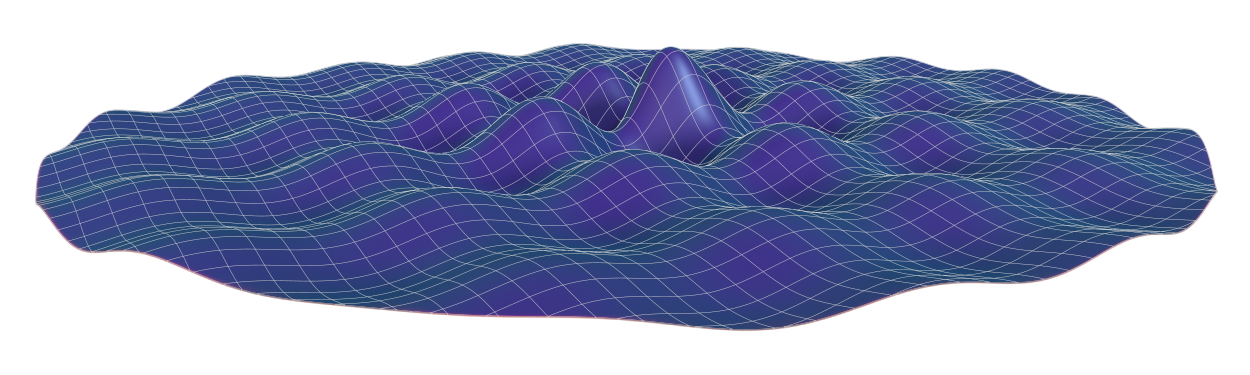
\includegraphics[width=6in]{resources/cover-render-lines-lowres.png}
	\end{center}
}
\renewcommand{\maketitlehookd}{
	\begin{center}
		
\includegraphics[width=1in]{resources/doclicense-CC-by-sa.pdf}
	\end{center}
}
\usepackage{lipsum} % Just to put in some text

\begin{document}

% no numbers on chapters here, etc.  it's the front matter!
\frontmatter
\begin{titlingpage}
	\calccentering{\unitlength}
	\begin{adjustwidth*}{\unitlength}{-\unitlength}
		\maketitle
	\end{adjustwidth*}
\end{titlingpage}

\clearpage

\tableofcontents*
\clearpage

\chapter{Introduction}
	
\emph{Multivariable Calculus} approaches the subject from a mathematical,
but not overly technical, perspective.  The key idea of calculus---chop
things into little pieces and put them together again---is emphasized
throughout.

\chapter{Licensing}
	This book would not be possible without the long tradition
of mathematical inquiry that came before.  And like the
ideas of mathematics, which are free for all to re-imagine,
re-use, and re-purpose, so too is this book.

This book is licensed under the Creative Commons By-Attribution
Share Alike 4.0 International license.  This gives you permission
to reuse, redistribute, and modify the contents of this book provided
you attribute a derived work appropriately and that you
license a derived work under the same terms.  For the full text
of the license, see Appendix \ref{APPENDIX-license}.

This book is a derived work of the Creative-Commons licensed
\emph{ISP Mathematics 281}\footnote{
\url{https://github.com/siefkenj/ISPMathematics281}
} multivariable calculus textbook by
Leonard Evans of Northwestern University.  The problems from this textbook
come from a variety of sources.  Unannotated problems come from \emph{ISP Mathematics 281}.
Problems with a superscript \openstax come from \emph{Calculus Volume 3}\footnote{
\url{https://openstax.org/details/calculus-volume-3}
} from the Openstax
project.  The Openstax problems are licensed under a Creative Commons By-Attribution
Non-Commercial Share Alike 4.0 license.  If you require this textbook to be fully open-source,
remove these problems.

\chapter{Contributors}
	% sorting code from
% http://tex.stackexchange.com/questions/121489/alphabetically-display-the-items-in-itemize
\newcommand{\sortitem}[2][\relax]{%
  \DTLnewrow{list}% Create a new entry
  \ifx#1\relax
    \DTLnewdbentry{list}{sortlabel}{#2}% Add entry sortlabel (no optional argument)
  \else
    \DTLnewdbentry{list}{sortlabel}{#1}% Add entry sortlabel (optional argument)
  \fi%
  \DTLnewdbentry{list}{description}{#2}% Add entry description
}
\newenvironment{sortedlist}{%
  \DTLifdbexists{list}{\DTLcleardb{list}}{\DTLnewdb{list}}% Create new/discard old list
}{%
  \DTLsort{sortlabel}{list}% Sort list
  \begin{itemize*}[label={\color{mypink}$\circ$}]%
    \DTLforeach*{list}{\theDesc=description}{%
      \item \theDesc}% Print each item
  \end{itemize*}%
}

This book is a collaborative effort.  The following people have contributed
to its creation:
\begin{quote}
\begin{sortedlist}
	\sortitem[Strauss]{Paul Strauss}
	\sortitem[Sigal]{Maxwell Sigal}
	\sortitem[Stakvileviciute]{Ieva Stakvileviciute}
	\sortitem[Cornish]{Dylaan Cornish}
	\sortitem[Dierksheide]{Julia Dierksheide}
	\sortitem[Soram]{Kim Soram}
	\sortitem[Riedel]{Kathryn Riedel}
\end{sortedlist}
{\color{mypink}$\circ$}
\end{quote}

% number the chapters and such
\mainmatter

\chapter{Preliminaries}
	\section{Mathematical Notation}
	Mathematics is a sophisticated and precise language, and
	we best not adventure into calculus without learning some
	basic words.

	The most basic mathematical word is that of a \emph{set}\index{set}.  
	A set is an unordered collection of distinct objects.  We won't try and pin
	it down more exactly than this---our intuition about collections
	of objects will suffice\footnote{ When you pursue more rigorous math,
	you rely on definitions to get yourself out of philosophical jams.  For instance,
	with our definition of set, consider ``the set of all sets that don't
	contain themselves.''  Such a set cannot exist!
	This is called \emph{Russel's Paradox}, and shows
	that if we start talking about sets of sets, we may need more than
	intuition.}. We write a set with curly-braces $\{$ and $\}$ and
	list the objects inside.  For instance
	\[
		\Set{1,2,3}.
	\]
	This would be read aloud as ``the set containing the elements $1$, $2$, and $3$.''
	The symbol $\in$\index{$\in$} is used to specify that some object is an element of a set, and
	$\notin$ is used to specify it is not.  For example,
	\[
		3\in\Set{1,2,3}\qquad 4\notin\Set{1,2,3}.
	\]
	Sets can contain mixtures of objects, including other sets.  For example,
	\[
		\Set{1,2,a,\Set{-70,\infty}, x}
	\]
	is a perfectly valid set.

	It is tradition to use capital letters to name sets.  So we might say $A=\{6,7,12\}$
	or $X=\{7\}$.  There is, however, a special set with a special name---the
	empty set.  The \emph{empty set} is the set containing no elements
	and is written $\emptyset$ or $\Set{}$.  Note that $\Set{\emptyset}$ is \emph{not}
	the empty set.  It is the set containing the empty set!  It is also traditional
	to call elements of a set \emph{points}\index{point} regardless of whether you
	consider them ``point-like'' objects.

	\subsection{Operations on Sets}
	If the set $A$ contains all the elements that the set $B$ does, we call $A$ a \emph{superset}\index{superset}
	and $B$ a \emph{subset}\index{subset}.  We'll give this a formal
	definition.
	\begin{definition}[Subset \& Superset]
		The set $B$ is a \emph{subset} of the set $A$, written $B\subseteq A$, if for all
		$b\in B$ we also have $b\in A$.  In this case, $A$ is called a \emph{superset}
		of $B$.\footnote{
			Some mathematicians use the symbol $\subset$ instead of $\subseteq$.}
	\end{definition}

	Some simple examples are $\Set{1,2,3}\subseteq \Set{1,2,3,4}$ and $\Set{1,2,3}\subseteq\Set{1,2,3}$.
	There's something funny about that last example, though.  Those two sets are not only subsets/supersets
	of each other, they're \emph{equal}.  As surprising as it seems, we actually need to define
	what it means for two sets to be equal.
	\begin{definition}[Set Equality]
		The sets $A$ and $B$ are \emph{equal}, written $A=B$, if $A\subseteq B$ and $B\subseteq A$.
	\end{definition}
	Having a definition of equality to lean on will help us when we need to prove things about sets.

	\begin{example}
		Let $A$ be the set of numbers that can be expressed
		as $2n$ for some whole number $n$, and let $B$ be the
		set of numbers that can be expressed as $m+1$ where $m$ is
		an odd whole number.  We will show $A=B$.

		First, let us show $A\subseteq B$.  If $x\in A$ then $x=2n$
		for some whole number $n$.  Therefore $x=2n=2(n-1)+1+1=m+1$ where
		$m=2(n-1)+1$ is, by definition, an odd number.  Therefore $x\in B$.

		Now we will show $B\subseteq A$.  Let $x\in B$.  By definition,
		$x=m+1$ for some odd $m$ and so by the definition of oddness, $m=2k+1$
		for some whole number $k$.  Thus 
		\begin{align*}
			x=m+1&=(2k+1)+1=2k+2\\
			&=2(k+1)=2n,
		\end{align*} where $n=k+1$, and so $x\in A$.  Since $A\subseteq B$
		and $B\subseteq A$, by definition $A=B$.
	\end{example}
	

	\subsubsection{Set-builder Notation}
	Specifying sets by listing all their elements can be a hassle, and if there are an infinite
	number of elements, it's impossible!  Fortunately, \emph{set-builder notation}\index{set-builder notation}
	solves these problems.
	If $X$ is a set, we can define a subset 
	\[
		Y= \Set{a\in X\given\text{some rule involving }a},
	\]
	which is read ``$Y$ is the set of $a$ in $X$ \emph{such that} some rule
	involving $a$ is true.''  If $X$ is intuitive, we may omit it and
	simply write $Y=\Set{a\given\text{some rule involving }a}$\footnote{ If you want
	to get technical, to make this notation unambiguous, you define a 
	\emph{universe of discourse}.  That is, a set $\mathcal U$ containing
	every object you might want to talk about.  Then $\Set{a\given\text{some rule involving }a}$
	is short for $\Set{a\in\mathcal U\given\text{some rule involving }a}$}.  You may equivalently
	use ``$|$'' instead of ``$:$'', writing $Y=\{a\,|\,\text{some rule involving }a\}$.

	\begin{example}
		The set $\Z$ is the set of integers (positive, negative,
		and zero whole numbers).  To define $E$ as the even integers,
		we could write
		\[
			E=\Set{n\in \Z\given n=2k\text{ for some }k\in \Z}.
		\]
		To define $P$ as the set of positive integers, we could write
		\[
			P=\Set{n\in\Z\given n>0}.
		\]
	\end{example}


	There are also some common operations we can do with two sets.
	\begin{definition}[Intersections \& Unions]
		Let $A$ and $B$ be sets. Then the \emph{intersection} of $A$ and $B$, written
		$A\cap B$, is defined by
		\[
			A\cap B=\Set{x\given x\in A\text{ and }x\in B}.
		\]
		The \emph{union} of $A$ and $B$, written $A\cup B$, is defined by
		\[
			A\cup B= \Set{x\given x\in A\text{ or } x\in B}.
		\]
	\end{definition}
	For example, if $A=\Set{1,2,3}$ and $B=\Set{-1,0,1,2}$, then $A\cap B=\Set{1,2}$ and $A\cup B=
	\Set{-1,0,1,2,3}$.  Set unions and intersections are \emph{associative}, which means it doesn't
	matter how you apply parentheses to an expression involving just unions or just intersections.
	For example $(A\cup B)\cup C=A\cup(B\cup C)$, which means
	we can give an unambiguous meaning to an expression like $A\cup B\cup C$ (just put
	the parentheses wherever you like).  But watch out, $(A\cup B)\cap C$ means something
	different than $A\cup(B\cap C)$!

	\begin{definition}[Set Subtraction]
		For sets $A$ and $B$, the \emph{set-wise difference}\index{set subtraction} between $A$ and $B$,
		written $A\backslash B$, is the set
		\[
			A\backslash B = \Set{x\given x\in A\text{ and }x\notin B}.
		\]
	\end{definition}
	\begin{definition}[Cardinality]
		For a set $A$, the \emph{cardinality}\index{cardinality} of $A$,
		written $\abs{A}$ is the number of elements in $A$.  If $A$
		contains infinitely many elements, we write $\abs{A}=\infty$.
	\end{definition}

	Let's define some notation for common sets.
	\begin{align*}
		\emptyset &= \Set{}\text{, the empty set}\\
		\N &= \Set{0,1,2,3,\ldots}=\Set{\text{natural numbers}}\\
		\Z &= \Set{\ldots, -3,-2,-1,0,1,2,3,\ldots}=\Set{\text{integers}}\\
		\Q &= \Set{\text{rational numbers}}\\
		\R &= \Set{\text{real numbers}}\\
		\R^n &= \Set{\text{vectors in $n$-dimensional Euclidean space}}\\
	\end{align*}

	Besides unions, there's another way to join sets together:
	\emph{products}\index{Cartesian product}\index{set product}.
	\begin{definition}[Cartesian Product]
		Given two sets $A$ and $B$, the \emph{Cartesian product} (sometimes
		shortened to \emph{product}) of the sets $A$ and $B$ is written
		$A\times B$ and defined to be
		\[
			A\times B = \Set{(a,b)\given a\in A\text{ and }b\in B}.
		\]
	\end{definition}
	The Cartesian product of two sets is the set of all ordered pairs of elements from
	those sets.  For example, 
	\[
		\Set{1,2}\times \Set{1,2,3}=\Set{(1,1),(1,2),(1,3),(2,1),(2,2),(2,3)}.
	\]
	You can repeat this operation more than once.   $\R\times \R\times \R$
	is the set of all triples of real numbers.  Extending power notation
	notation, if you take the Cartesian product of a set
	with itself some number of times, you can represent it with
	an exponent.  Thus, $\R\times \R\times \R$ can be written as $\R^3$, which is a set we've
	seen before%
	\footnote{
		If you're scratching your head saying, ``I thought $\R^3$ was vectors in $3$-dimensional
		space.  How do we know that's the same thing as triples of real numbers?'' your mind
		is keen.  This is a theorem of linear algebra.
	}.

	\subsection{Functions}
	You're probably used to seeing functions like $f(x)=x^2$, but it's worth reviewing some of the concepts
	and terminology associated with functions.

	\begin{definition}[Function]
		A \emph{function}\index{function} with \emph{domain}\index{domain} the 
		set $A$ and \emph{co-domain}\index{co-domain} the set $B$ is an object that
		associates every point in the set $A$ with \emph{exactly one} point in the set $B$.
	\end{definition}

	If a function $f$ has domain $A$ and co-domain\footnote{ Some
	people use the word \emph{range} interchangeably with co-domain.} $B$,
	we notate this by writing $f:A\to B$.
	If we want to further specify what the function $f$ actually is, we need to
	express how $f$ associates each point in $A$ to a point in $B$.  This can be done
	with an equation.  For example, we could define the function $f:\R\to\R$ by
	\[
		f(x)=2x,
	\]
	which says that each real number gets associated to its double.  We can notate
	the same thing using a special type of arrow: ``$\mapsto$''.  Now we might write
	\[
		f:\R\to\R\text{ where } x\mapsto 2x,
	\]
	which is read ``$f$ is a function from $\R$ to $\R$ where $x\in \R$ gets mapped to $2x$.''

	
	Note that every point in the co-domain of a function doesn't need to get mapped
	to.  For example $g:\R\to\R$ given by $g(x)=x^2$ outputs only non-negative numbers,
	but it is still valid to specify $\R$ as the co-domain.  However, if we wanted
	to make a point of it, we are perfectly justified in writing $g:\R\to[0,\infty)$
	when defining $g$.

	Many common math operations give rise to functions.  For example,  
	$f(x)=\sqrt{x}$ is the familiar
	square root function.  Sometimes, when we wish to talk about a function
	for which notation already exists, we will put a ``$\ \cdot\ $'' where we would
	normally put a variable.  Thus, we might say, ``$\sqrt{\:\cdot\:}$ is the square
	root function.''\footnote{ Since $\sqrt{x}$ is ``the square root of the quantity
	$x$,'' it is technically a quantity and not a function.  This is why we write $\ \cdot\ $ instead
	of $x$ when we want to refer to the square root \emph{function}.
	}

	\begin{definition}[Range]
		The \emph{range}\index{range} of a function $f:A\to B$
		is the set of all outputs of $f$.  That is
		\[
			\Range f = \Set{y\in B\given y=f(x)\text{ for some }x\in A}.
		\]
	\end{definition}
	\begin{definition}[Image]
		Let $f:A\to B$ be a function.
		The \emph{image}\index{image} of a set $X\subseteq A$, written $f(X)$ is
		defined by
		\[
			f(X)=\Set{y\in B\given y=f(x)\text{ for some }x\in X}.
		\]
	\end{definition}

	We see that if $f:A\to B$, $\Range f = f(A)$.  In words, the range of $f$ is the image
	of its domain.  This language will become useful when we think of functions as transformations
	that move or bend space.  If $f:\R^2\to\R^2$ is a function that warps the Cartesian plane,
	then the image of $X$ under $f$ could be visualized by painting $X$ on the Cartesian plane,
	warping the whole plane, and then looking at the resulting, painted shape.  


	Closely related to images, we have the idea of \emph{restriction}\index{restriction}.
	Suppose $f:\R^2\to\R$ is defined by $f(x,y)=xy$, but we were only really interested in $f$ on the unit circle, $\mathcal C$.
	In this case, we might say $f$ attains a maximum on $\mathcal C$, or $f$ 
	\emph{restricted to} $\mathcal C$ attains a maximum, even though $f$ itself is unbounded.
	This idea comes up often enough to deserve its own notation.

	\begin{definition}[Restriction]
		If $f:A\to B$ and $X\subseteq A$, the \emph{restriction}\index{restriction}
		of $f$ to $X$ is written 
		$f\big|_X$ and is defined to be the function $g:X\to A$ where $x\mapsto f(x)$.
	\end{definition}

	The last important function-related ideas for us are function composition and inverses.
	Given two functions $f:A\to B$ and $g:B\to C$, we can \emph{compose}\index{function composition}
	$g$ and $f$ to get a new function.
	\begin{definition}[Composition]
		Given two functions $f:A\to B$ and $g:B\to C$, the \emph{composition} of
		$g$ and $f$, written $g\circ f$, is the function $h:A\to C$ where 
		$x\mapsto g(f(x))$.
	\end{definition}
	Note that the composition $g\circ f$ has the domain of $f$ and the co-domain of $g$.
	When a point is fed into $g\circ f$, it moves from $A\to B\to C$.  The composition
	$g\circ f$ only makes sense because the outputs of $f$ are allowed as inputs to $g$.
	If we wrote $f\circ g$, it wouldn't mean much, because $g$ outputs points in $C$ and $f$
	has no idea what to do with points in $C$.\footnote{
		It seems a little backward to write $f:A\to B$, $g:B\to C$ and then
		write $g\circ f$ instead of $f\circ g$.  You can thank Euler for that.
		He decided to write functions with their input on the right instead of
		the left.  If we wrote functions backwards, like $((x)f)g$ for ``$g$ of $f$ of $x$,''
		they we could just \emph{follow the arrows} and life would be simpler.
	}

	Inverses relate to composition and the \emph{identity function}\index{identity function}, the function
	that does nothing to its inputs.
	\begin{definition}[Identity Function]
		The \emph{identity function} $\Id:A\to A$ is defined by the relation
		\[
			\Id(x)=x
		\]
		for all $x\in A$.
	\end{definition}
	Notice that for every set, that set
	is the domain of an identity function.  Since the domain
	and co-domain of a function are part of its definition, we don't want to confuse them.
	After all, $f:\Set{0,1}\to \Set{0,1}$ given by $f(x)=x^2$ is a different function from $f:\R\to\R$
	given by $f(x)=x^2$.  For the special case of the identity function, we sometimes write
	the domain of the function as a subscript.  That is, 
	for $\Id:A\to A$ we'd write $\Id_A$ so it
	doesn't get confused with $\Id:B\to B$, which we'd write $\Id_B$.

	\begin{definition}[Inverse Function]
		Let $f:A\to B$ be a function.  If there exists a function $g:B\to A$ such that
		\[
			f\circ g=\Id_B\qquad\text{and}\qquad g\circ f=\Id_A,
		\]
		we say $f$ is \emph{invertible} and we call $g$ the \emph{inverse} of $f$.
		If $f$ is invertible, we notate its inverse by $f^{-1}$.
	\end{definition}

	Inverses can be tricky some times.  For example, consider $f(x)=x^2$ and $g(x)=\sqrt{x}$.
	Here $g\circ f(x)=\sqrt{x^2}=\abs{x}$ and $f\circ g(x) = \sqrt{x}^2=x$.  What's the deal?
	Well, it's all about domains.  $f:\R\to[0,\infty)$ and $g:[0,\infty)\to[0,\infty)$.
	So, the domain of $g\circ f$ is $\R$ and the domain of $f\circ g$ is $[0,\infty)$.  The
	domains are different, and indeed $f$ is not invertible.  However, $g$ \emph{is} invertible,
	and $g^{-1}=f\big|_{[0,\infty)}$.  If we only input non-negative numbers into $f$, then
	$f$ exactly undoes what $g$ did.  This subtle domain trickery can cause us a lot
	of headaches if we're not used to thinking carefully, and many of our favorite functions
	that we're used to calling ``inverse functions'' are actually only inverses when paired with
	specific domains.

\section{Proof}
	Mathematics has the highest standard of proof of any field.  In the Platonic ideal
	of mathematics, we start from some basic assumptions, called \emph{axioms}, that we have
	all agreed upon.  Then from those axioms, using the rules of logic, we deduce \emph{theorems}.
	Every single mathematical statement we make can be traced back from theorem to theorem
	and eventually to our initial axioms.

	This is contrary to other disciplines, like physics.
	In physics, based on observation, we construct
	\emph{laws}.  Laws in physics are like
	axioms in mathematics, but they have an important difference---they
	can be disproven by observation.  A mathematical axiom can never be disproven.  One can
	certainly argue that an axiom is not \emph{useful} or not \emph{interesting}, but you
	cannot say it's \emph{wrong}\footnote{
		There are multiple ways to axiomatize geometry.  In
		Euclidean geometry every pair of lines either coincides, intersects in
		exactly one place, or does not intersect.  In spherical
		geometry, every pair of lines either coincides or intersects in exactly two places.  
		Euclidean geometry is useful when your space looks flat.  Spherical
		geometry is useful when your space is the surface of a sphere (like 
		the Earth).
		Is one of these more \emph{right} than the other?  They're certainly
		contradictory.
	}.
	Of course, as human practitioners, we may misuse logic and be wrong ourselves, but that
	is no fault of the axioms.

	But now, let's deviate from philosophical perfection and visit reality.
	In reality, \emph{mathematics is a human pursuit to understand relationships
	between ideas and their consequences}.  The key there is that \emph{humans} do
	mathematics to \emph{understand} relationships.  If a theorem in math can
	ultimately be reduced to logical statements about axioms, but the argument is
	100000 steps long, it doesn't help a human understand why something is true.
	Instead, a shorter argument that skips over some steps is more useful to us.
	And, indeed, most of our mathematics to date skips over some steps\footnote{
		There are some projects to prove all of mathematics directly from
		the axioms using computer assistance.  They've made progress, but there
		are still theorems in calculus that have not been reduced to the
		axioms.  We believe that they \emph{could be} reduced to the axioms,
		but no one has taken the time to do so.}.

	We call a correct mathematical argument a \emph{proof}.  A proof starts
	from a set of assumptions, and following the rules of logic, arrives at a conclusion.
	Strictly speaking, a proof doesn't need to make sense or show motivation,
	applications, or examples.  It just has to be a sequence of correct logical steps.
	However, for us, as humans studying mathematics, we prove things for two reasons:
	to understand why things are true and to avoid making mistakes.

	Reconciling these two goals can be very hard for a novice mathematician.  If you include
	\emph{all} the steps, it won't help with understanding, but if you don't include enough
	steps, the argument may not be convincing and might contain mistakes.  
	Even professionals struggle to balance
	these competing goals, and how you balance those goals depends on your audience---if you're
	trying to convince your math professor of something your proof will need to have more
	detail than if you were trying to convince your friend (mathematicians are very skeptical!).

	Enough talk, let's go through a 2000-year-old example of a proof.
	\begin{theorem}
		There is no rational number $p/q$ such that $(p/q)^2=2$.
	\end{theorem}
	\begin{proof}
		If $p/q$ is a rational number, it can be expressed
		in lowest terms.
		Suppose $p/q$ is in lowest terms and $(p/q)^2=2$.  Then $p^2=2q^2$ and so $p^2$ is even.  Since
		$p^2$ is even, it must be that $p$ is even, and so by definition,
		$p=2m$ for some integer $m$.  Now,
		\[
			\frac{p^2}{q^2}=\frac{(2m)^2}{q^2}=\frac{4m^2}{q^2}=2,
		\]
		with the last equality following by assumption.  Multiplying both sides by $q^2$
		and dividing by $2$ we arrive at the equation
		\[
			2m^2=q^2,
		\]
		and so $q^2$ is even which means $q$ is even.  By definition, this means $q=2n$ for some integer $n$.
		But now,
		\[
			\frac{p}{q}=\frac{2m}{2n}
		\]
		is not in lowest terms!  This is a contradiction and so it cannot be that $(p/q)^2=2$.
	\end{proof}
	This is nearly identical to the argument the ancient Greeks gave.  It's elegant, beautiful,
	and convincing.  But, if we look closer, it does skip some steps.  For example, it relies on
	the fact that there is such a thing as \emph{lowest terms}.  This is something that would
	need to be proven---a priori, the conclusion of the proof could be that the assumption
	that $p/q$ could be in lowest terms is false.  
	
	You will not, overnight,
	become a master at understanding
	what steps you can leave out and what steps you must show.  However, with feedback,
	you'll get better.
	For a detailed guide on writing good proofs, please see Appendix \ref{APPENDIX-proofstyle}.


	\clearpage
\chapter{Vectors}
	A \emph{vector}\index{vector} is a quantity which is characterized by
a \emph{magnitude} and a \emph{direction}.   Many quantities are best
described by vectors rather than
numbers.  For example, when driving a car,
 it may be sufficient to
know your speed, which can be described by a single number,
 but the motion of an airplane must be described
by a vector quantity---velocity---which takes into account its
direction as well as its speed.

Ordinary numerical quantities are called \emph{scalars}\index{scalar}
when we want to emphasize that they are not vectors.

Whereas numbers allow us to specify relationships between single quantities
(put in twice as much flour as sugar), vectors will allow us to specify
relationships between geometric objects in space\footnote{
	Though in this book we will treat vectors as intertwined with Euclidean
	space, they are much more general.  For instance, someone's internet
	browsing habits could be described by a vector---the topics they
	find most interesting might be the ``direction'' and the amount
	of time they browse might be the ``magnitude.''
}.  If we have two points, $P=(1,1)$ and $Q=(3,2)$, we specify the
\emph{displacement}\index{displacement} from $P$ to $Q$ as a vector.

\begin{center}
	\usetikzlibrary{patterns,decorations.pathreplacing}
	\begin{tikzpicture}
		\coordinate (A) at (1,1);
		\coordinate (B) at (3,2);
		\begin{axis}[
		    anchor=origin,
		    disabledatascaling,
		    xmin=-1,xmax=5,
		    ymin=-1,ymax=3,
		    x=1cm,y=1cm,
		    grid=both,
		    grid style={line width=.1pt, draw=gray!10},
		    %major grid style={line width=.2pt,draw=gray!50},
		    axis lines=middle,
		    minor tick num=0,
		    enlargelimits={abs=0.5},
		    axis line style={latex-latex},
		    ticklabel style={font=\tiny,fill=white},
		    xlabel style={at={(ticklabel* cs:1)},anchor=north west},
		    ylabel style={at={(ticklabel* cs:1)},anchor=south west}
		]

		\draw [mypink,fill] (A) circle (1.5pt) node [below right] {$P$};
		\draw [mypink,fill] (B) circle (1.5pt) node [below right] {$Q$};
		\draw[->,thick,myred!60!white] (A) -- (B) node [midway,above,yshift=2pt] {$\overrightarrow{PQ}$};

		\end{axis}
%		\begin{axis}[
%			anchor=origin,
%			disabledatascaling,
%			% tell pgfplots to use the same unit vectors
%			% as tikz:
%			x=1cm,y=1cm,
%			xmin=-1,xmax=4, ymin=-1,ymax=4,grid=both]
%			% this uses the point defined OUTSIDE of the axis
%			\draw [blue,fill] (Point) circle (2pt)
%			node [right] {(1,2)};
%			% this uses a TIKZ coordinate (2,0) in the axis:
%			\draw [blue,fill] (2,0) circle (2pt)
%			node [right] {(2,0)};
%			% this here will always work inside of an axis:
%			\draw [blue,fill] (-1,0) circle (2pt)
%			node [right] {(-1,0)};
%		\end{axis}
	\end{tikzpicture}
\end{center}

We notate the displacement vector form $P$ to $Q$ by $\overrightarrow{PQ}$.
The magnitude of $\overrightarrow{PQ}$ is given by the Pythagorean theorem
to be $\sqrt{5}$ and its direction is specified by the directed line segment from
$P$ to $Q$.


\section{Vector Notation}
There are many ways to represent vector quantities in writing.  If
we have two points, $P$ and $Q$, we write $\overrightarrow{PQ}$ to represent the
vector from $P$ to $Q$.  Absent of points, bold-faced letters or a letter
with an arrow over it are the most common typographical representations of vectors.
For example, $\vec a$ or $\mathbf{a}$ may both be used to represent the vector
quantity named ``$a$.''  In this book we will use $\vec a$ to represent a vector.
The notation $\norm{\vec a}$\index{$\norm{\:\cdot\:}$}\index{magnitude}\index{norm}
represents the magnitude of the vector $\vec a$, which is sometimes called
the \emph{norm} of $\vec a$.

Graphically, vectors are represented as directed line segments (a
line segment with an arrow at one end).  The endpoints of the segment are called the 
\emph{initial
point} (the base) and the \emph{terminal point} (the tip) of the vector.

\begin{center}
	\usetikzlibrary{patterns,decorations.pathreplacing}
	\begin{tikzpicture}
		\coordinate (A) at (1,1);
		\coordinate (B) at (-.5,2);

		\draw [mypink,fill] (A) circle (1.5pt) node [right] {initial point};
		\draw [mypink,fill] (B) circle (1.5pt) node [left] {terminal point};
		\draw[->,thick,myred!60!white] (A) -- (B);
	\end{tikzpicture}
\end{center}

Let $A=(1,1)$, $B=(3,2)$, $X=(1,0)$, and $Y=(3,1)$ and consider the vectors
$\vec a = \overrightarrow{AB}$ and $\vec x=\overrightarrow{XY}$.  Are these
the same or different vectors?  If we drew them as directed line segments,
the drawings would be distinct.  However, both $\vec a$ and $\vec x$ have equivalent
magnitudes and directions.  Thus, $\vec a$ and $\vec x$ are \emph{equivalent},
and we would be justified writing $\vec a=\vec x$.

\begin{center}
	\usetikzlibrary{patterns,decorations.pathreplacing}
	\begin{tikzpicture}
		\coordinate (A) at (2,1);
		\begin{axis}[
		    anchor=origin,
		    disabledatascaling,
		    xmin=-1,xmax=5,
		    ymin=-1,ymax=3,
		    x=1cm,y=1cm,
		    grid=both,
		    grid style={line width=.1pt, draw=gray!10},
		    %major grid style={line width=.2pt,draw=gray!50},
		    axis lines=middle,
		    minor tick num=0,
		    enlargelimits={abs=0.5},
		    axis line style={latex-latex},
		    ticklabel style={font=\tiny,fill=white},
		    xlabel style={at={(ticklabel* cs:1)},anchor=north west},
		    ylabel style={at={(ticklabel* cs:1)},anchor=south west}
		]

			\draw[->,thick,myred!60!white] (1,1) -- +(A) node [midway,above,xshift=-8pt] {$\vec x=\overrightarrow{AB}$};
			\draw[->,thick,mypink] (1,0) -- +(A) node [midway,above,xshift=-8pt] {$\vec x=\overrightarrow{XY}$};
		%\draw[->,thick,myred!60!white] (3,1) -- +(A) node [midway,above,yshift=2pt] {$\vec x$};

		\end{axis}
	\end{tikzpicture}
\end{center}

Alternatively, we could consider the \emph{rooted vector}\index{rooted vector}
$\vec a$ rooted at the point $A$.  In this terminology, $\vec a$ rooted
at $A$ is \emph{different} than $\vec a$ rooted at $X$.  This idea
of rooted vectors will occasionally be useful, but our primary study will be unrooted
vectors.

\subsection{Vectors and Points}
The distinction between vectors and points is sometimes nebulous because
they are so closely related to each other.  A \emph{point}\index{point}
in Euclidean space specifies an absolute position whereas a vector
specifies a magnitude and direction.  However, given a point $P$,
one associates $P$ with the vector $\vec p=\overrightarrow{OP}$, where $O$
is the origin.  Similarly, we associate the vector $\vec v$ with
the point $V$ so that $\overrightarrow{OV}=\vec v$.
Thus, we have a way to unambiguously go back and forth between vectors and 
points\footnote{ Mathematically, we say there is an \emph{isomorphism} between
vectors and points.}.  As such, \emph{we will treat vectors and points
as interchangeable}.

\begin{exercises}
	\begin{enumerate}
		\item   Find the vector of the form $a\xhat + b\yhat + c\zhat$ that is represented by an 
			arrow from the point $P(7, 2, 9)$ to the point $Q(-2, 1, 4)$.
	\end{enumerate}
\end{exercises}
\begin{openstaxexercises}
	\begin{enumerate}
		\item   For the following exercises, consider points $P(-1,3)$, $Q(1,5)$, and $R(-3,7)$.
			Determine the requested vectors and express each of them i. in component form
			and ii. by using the standard unit vectors. 
			\begin{enumerate}
				\item $\overrightarrow{PQ}$	
				\item $\overrightarrow{PR}$
				\item $\overrightarrow{QP}$
				\item $\overrightarrow{RP}$
			\end{enumerate}
	\end{enumerate}
\end{openstaxexercises}


\section{Vector Arithmetic}
Vectors provide a natural way to give directions.
For example, suppose $\xhat$ points one mile eastwards and $\yhat$
points one mile northwards.  Now, if you were standing at the origin
and wanted to move to a location 3 miles east and 2 miles north, you might say:
``Walk 3 times the length of $\xhat$  in the $\xhat$ direction and 2 times
the length of $\yhat$ in the $\yhat$ direction.''  Mathematically, we express this
as
\[
	3\xhat+2\yhat.
\]
Of course, we've incidentally described a new vector.  Namely, let $P$
be the point at 3-east and 2-north.  Then
\[
	\overrightarrow{OP}=3\xhat+2\yhat.
\]
If the vector $\vec r$ points north but has a length of 10 miles, we have
a similar formula:
\[
	\overrightarrow{OP}=3\xhat+\tfrac{1}{5}\vec r,
\]
and we have the relationship $\vec r=10\yhat$.
Our notation here is very suggestive.  Indeed, if we could make
sense of what $\alpha\vec v$ is for any scalar $\alpha$ and vector
$\vec v$, and we could make sense of what $\vec v+\vec w$
means for any vectors $\vec v$ and $\vec w$, we would be able to
do algebra with vectors.  We might even say we have \emph{an algebra
of vectors}.

Intuitively, for a vector $\vec v$ and a scalar $\alpha>0$, the
vector $\vec w=\alpha\vec v$ should point in the same direction as
$\vec v$ but have magnitude scaled up by $\alpha$.  That is, $\norm{\vec w}=\alpha\norm{\vec v}$.
Similarly, $-\vec v$ should be the vector of the same length as $\vec v$ but
pointing in the exact opposite direction.

\begin{center}
	\usetikzlibrary{patterns,decorations.pathreplacing}
	\begin{tikzpicture}
		\coordinate (A) at (2,1);

		\draw[->,thick,green!50!black] (1,0) -- +($(A) + (A)$) node [midway,below right ] {$2\vec v$};
		\draw[->,thick,myred!60!white] (0,0) -- +(A) node [midway,above left] {$\vec v$};
		\draw[->,thick,mypink] (-1,0) -- +($-.5*(A)$) node [midway,right,xshift=4pt] {$-\tfrac{1}{2}\vec v$};
	\end{tikzpicture}
\end{center}

For two vectors $\vec u$ and $\vec v$, the sum $\vec w=\vec u+\vec v$
should be the displacement vector created by first displacing along $\vec u$
and then displacing along $\vec v$.

\begin{center}
	\usetikzlibrary{patterns,decorations.pathreplacing}
	\begin{tikzpicture}
		\coordinate (A) at (1,1);
		\coordinate (B) at (-.5,2);
		\coordinate (C) at (3,3);

		%\draw [mypink,fill] (A) circle (1.5pt) node [right] {initial point};
		%\draw [mypink,fill] (B) circle (1.5pt) node [left] {terminal point};
		\draw[->,thick,myred!60!white] (A) -- (B) node [midway,below left] {$\vec u$};
		\draw[->,thick,mypink] (B) -- (C) node [midway,above left] {$\vec v$};
		\draw[->,thick,green!50!black] (A) -- (C) node [midway,right] {$\vec w=\vec u+\vec v$};
	\end{tikzpicture}
\end{center}

Now, there is one snag.  What should $\vec v+(-\vec v)$ be?  Well, first we
displace along $\vec v$ and then we displace in the exact opposite direction 
by the same amount.  So, we have gone nowhere.  This corresponds to a displacement
with zero magnitude.  But, what direction did we displace?  Here we make a philosophical
stand.
\begin{definition}[Zero Vector]
	The \emph{zero vector}\index{zero vector}, notated as $\vec 0$\index{$\vec 0$}, 
	is the vector with no magnitude.
\end{definition}
We will be pragmatic about the direction of the zero vector and say,
\emph{the zero vector does not have a well-defined direction}\footnote{
	In the mathematically precise definition of vector, the idea of ``magnitude''
	and ``direction'' are dropped.  Instead, a set of vectors is defined to be
	a set over which you can reasonably define addition and scalar multiplication.
}.  That means
sometimes we consider the zero vector to point in every direction and sometimes
we consider it to point in no directions.  It depends on our mood---but we must
never talk about \emph{the} direction of the zero vector, since it's not defined.

We need the zero vector if we are to make precise mathematical
sense of vector arithmetic.
Further along this line of thinking, we can define precisely how vector arithmetic
should behave.  Specifically, if $\vec u$, $\vec v$, $\vec w$ are vectors and $\alpha$ and $\beta$
are scalars, the
following conditions should be satisfied:
\begin{align*}
	(\vec u+\vec v)+\vec w&=\vec u+(\vec v+\vec w)\tag{Associativity}\\
	\vec u+\vec v&=\vec v+\vec u\tag{Commutativity}\\
	\alpha(\vec u+\vec v)&=\alpha\vec u+\alpha \vec v\tag{Distributivity}
\end{align*}
and 
\begin{align*}
	(\alpha\beta)\vec v&=\alpha(\beta \vec v)\tag{Associativity II}\\
	(\alpha+\beta)\vec v&=\alpha\vec v+\beta \vec v\tag{Distributivity II}
\end{align*}

Indeed, if we intuitively think about vectors in flat (Euclidean) space,
all of these properties are satisfied\footnote{
	If we deviate from flat space, some of these
	rules are no longer respected.  Consider moving 100 miles
	north then 100 miles east on a sphere.  Is this the
	same as moving 100 miles east and then 100 miles north?
}.  From now on, these properties of vector operations will be considered
the 
\emph{laws (or axioms) of vector arithmetic}.

We'll be talking about these vector operations (scalar multiplication and
vector addition) a lot.  So much so that the concept is worth naming.
\begin{definition}[Linear Combination]
	A \emph{linear combination} of the vectors $\vec v_1,\ldots \vec v_n$
	is any vector expressible as
	\[
		\alpha_1\vec v_1+\cdots +\alpha_n\vec v_n,
	\]
	where $\alpha_1,\alpha_2,\ldots,\alpha_n$ are scalars.
\end{definition}


We've given laws for linear combinations of vectors, but what about
for magnitudes of vectors?  We'd like the magnitude (or norm\index{norm}) of a vector to obey
the following laws.
\begin{align*}
	\norm{\vec v} &\geq 0\tag{Non-negativity}\\
	\norm{\vec v} &= 0\text{ only when}\vec v=\vec 0\tag{Definiteness}\\
	\norm{\alpha\vec v}&=\abs{\alpha}\norm{\vec v}\tag{Homogeneity}\\
	\norm{\vec v+\vec w}&\leq\norm{\vec v}+\norm{\vec w}\tag{Triangle Inequality}
\end{align*}
for all $\vec v$, $\vec w$, and scalars $\alpha$.  Any function on vectors satisfying
those four properties is called a \emph{norm}, and our usual notion
of length in three-dimensional space indeed obeys those properties\footnote{
	The Euclidean norm comes from the Pythagorean theorem $a^2+b^2=c^2$.
	However, by changing the exponent, we have a whole family of norms
	coming from the equations $\abs{a}^p+\abs{b}^p=\abs{c}^p$.
}.

Homogeneity is a particularly special property of a norm.  It allows us
to easily create \emph{unit vectors}.
\begin{definition}[Unit Vector]
	A \emph{unit vector}\index{unit vector} is a vector $\vec u$
	satisfying $\norm{\vec u}=1$.
\end{definition}
Unit vectors are handy because if $\vec u$ is a unit vector, then $k\vec u$
has length $\abs{k}$.  Further, we can always turn a vector into a unit vector.
\begin{example}
	The vector $\vec v/\norm{\vec v}$ is always a unit vector in the direction
	of $\vec v$.  Computing,
	\[
		\norm*{\frac{\vec v}{\norm{\vec v}}} = \abs*{\frac{1}{\norm{\vec v}}}\norm{\vec v}=
		\frac{1}{\norm{\vec v}}\norm{\vec v}=1.
	\]
\end{example}


\section{Coordinates}
Recall that a rectangular coordinate system in the plane is specified by choosing
an origin $O$ and then choosing two perpendicular axes meeting at
the origin.  These axes are chosen in some order so that we know which
axis (usually the $x$-axis) comes first and which (usually the
$y$-axis) second.   Note that there are many different coordinate systems
which could be used although we often draw pictures
as if there were only one.

In physics, one often has to think carefully about the
coordinate system because
choosing one appropriately may greatly simplify the
analysis.  Note that axes for coordinate systems are usually drawn with 
\emph{right-hand orientation}, where the right angle from the positive
$x$-axis to the positive $y$-axis is in the counter-clockwise
direction.  However, it would be equally valid to use the
\emph{left-hand orientation} in which that angle is in the
clockwise direction.  One can easily switch the orientation of
a coordinate system by reversing one of the axes\footnote{
	The concept of
orientation is quite fascinating and it arises in mathematics,
physics, chemistry, and even biology in many interesting ways.
Note that almost all of us base our intuitive concept of orientation
on our inborn notion of ``right'' versus ``left''.}.

\begin{center}
	\begin{tikzpicture}
		\begin{axis}[
		    anchor=origin,
		    disabledatascaling,
		    xmin=-1,xmax=3,
		    ymin=-1,ymax=2,
		    x=1cm,y=1cm,
		    grid=both,
		    grid style={line width=.1pt, draw=gray!10},
		    %major grid style={line width=.2pt,draw=gray!50},
		    axis lines=middle,
		    minor tick num=0,
		    enlargelimits={abs=0.5},
		    axis line style={->},
		    ticklabel style={font=\tiny,fill=white},
		    xlabel={$x$}, ylabel={$y$},
		    xlabel style={at={(ticklabel* cs:1)},anchor=west},
		    ylabel style={at={(ticklabel* cs:1)},anchor=south}
		]

		\end{axis}
		\draw[] (.2,1) node[right,myorange!60!black] {Right Handed};
	\end{tikzpicture}
	\hspace{1cm}
	\begin{tikzpicture}
		\begin{axis}[
		    anchor=origin,
		    disabledatascaling,
		    xmin=-1,xmax=3,
		    ymin=-1,ymax=2,
		    x=1cm,y=1cm,
		    x dir=reverse,
		    grid=both,
		    grid style={line width=.1pt, draw=gray!10},
		    %major grid style={line width=.2pt,draw=gray!50},
		    axis lines=middle,
		    minor tick num=0,
		    enlargelimits={abs=0.5},
		    axis line style={->},
		    ticklabel style={font=\tiny,fill=white},
		    xlabel={$x$}, ylabel={$y$},
		    xlabel style={at={(ticklabel* cs:1)},anchor=west},
		    ylabel style={at={(ticklabel* cs:1)},anchor=south}
		]

		\end{axis}
		\draw[] (-.4,1) node[left,mypink] {Left Handed};
	\end{tikzpicture}
\end{center}

For any coordinate system, there are special vectors
associated with it.  For the plane, the vector pointing one unit along
the positive $x$-axis is called $\xhat$ and the vector pointing one unit along
the positive $y$-axis is called $\yhat$.  The vectors $\xhat$ and $\yhat$ are
called the \emph{standard basis}\index{standard basis} vectors for $\R^2$.

Notice that every point (or vector) in the plane can be represented
as a linear combination of $\xhat$ and $\yhat$, and the vector
$\alpha\xhat+\beta\yhat$ is the vector $\overrightarrow{OP}$ where
$P=(\alpha,\beta)$.  Now, to state an intuitive fact:  if $\vec w$ is
a vector in the plane, \emph{there is
only one way to write a vector as a linear combination of
$\xhat$ and $\yhat$}.  This means, if $\vec w=\alpha\xhat+\beta\yhat$,
the pair $(\alpha,\beta)$ captures all information\footnote{
	Maybe you already knew this because the point $(\alpha,\beta)$
	is described by the pair of numbers $(\alpha,\beta)$, duh!
	But consider, what would we do if we didn't know about coordinates
	at all? One approach is to \emph{define} coordinates in terms
	of vectors, which is really what we're doing.
} about $\vec w$.


For a vector $\vec w=\alpha\xhat+\beta\yhat$,
we call the pair $(\alpha,\beta)$  the 
\emph{components}\index{components} of the vector $\vec w$.  There
are many equivalent notations used to represent components.
\begin{center}
	\begin{tabular}{c p{5cm}}
		$(\alpha,\beta)$ & parenthesis\\
		$\langle \alpha,\beta\rangle$ & angle brackets\\
		$\mat{\alpha&\beta}$ & square brackets in a row (a row matrix)\\
		$\mat{\alpha\\\beta}$ & square brackets in a column (a column matrix)\\
	\end{tabular}
\end{center}

Given what we now know about representing vectors and their equivalency
with points, we can now dissect the notation $\R^2$.
On the one hand, $\R^2$ is the set of vectors in two-dimensional Euclidean
space.  On the other hand $\R^2=\R\times \R$ is the set of all pairs of real 
numbers.  Via the use of coordinates, we know these concepts represent the
same thing!
Further,
since vectors in $\R^2$ are equivalent to their representation in coordinates,
we will often write
\[
	\vec v=(\alpha,\beta)
\]
as a shorthand for $\vec v=\alpha\xhat+\beta\yhat$.


Breaking vectors into components, and in particular, viewing vectors as linear
combinations of the standard basis vectors, allows us to solve problems that were
difficult before.  For instance, suppose we have vectors $\vec v$ and $\vec w$.
How can we compute $\norm{\vec v+\vec w}$?  With components, it's easy.

\begin{example}
	\label{EXAMPLE-vecadd}
	Suppose $\vec v=\alpha_1\xhat+\beta_1\yhat$ and $\vec w=\alpha_2\xhat+\beta_2\yhat$.
	By the laws of vector arithmetic we have
	\[
		\vec v+\vec w=(\alpha_1\xhat+\beta_1\yhat)+(\alpha_2\xhat+\beta_2\yhat)
		=(\alpha_1+\alpha_2)\xhat+(\beta_1+\beta_2)\yhat.
	\]
	Now, since $\xhat$ and $\yhat$ are orthogonal to each other,
	the Pythagorean theorem gives
	\[
		\norm{\vec v+\vec w} = \sqrt{(\alpha_1+\alpha_2)^2+(\beta_1+\beta_2)^2}.
	\]
\end{example}

Writing things in terms of the standard basis allowed us to make easy work
of computing $\norm{\vec v+\vec w}$ in Example \ref{EXAMPLE-vecadd}.  We can
use the laws of vector arithmetic to produce rules for working with components.

The rules are are likely familiar:
\[
	\mat{a\\b}+\mat{\alpha\\\beta} = \mat{a+\alpha\\b+\beta}
	\qquad\text{and}\qquad
	\alpha \mat{a\\b}=\mat{\alpha a\\\alpha b}.
\]

\begin{exercise}
	Prove the rules for adding the component representation
	of vectors and multiplying the component representation 
	of vectors directly from the laws of vector arithmetic.
\end{exercise}

Armed with these rules, we will be able to tackle sophisticated vector
problems.

\subsection{Three-dimensional Coordinates}
In three-dimensional space, the story is very similar.  Again, we imagine
three perpendicular axes, the $x$, $y$, and $z$ axes.  
To draw consistent
pictures, we have a notion of a right-handed three-dimensional coordinate
system given by the \emph{right-hand rule}.

\begin{center}
	\usetikzlibrary{patterns,decorations.pathreplacing}
	\hspace{-3.5cm}
	\begin{tikzpicture}
		\begin{axis}[
		    anchor=origin,
		    scale mode=scale uniformly,
			scale=2,
		    %disabledatascaling,
		    xmin=-2,xmax=2,
		    ymin=-2,ymax=2,
		    zmin=-2,zmax=2,
		    %x=1cm,z=1cm,y=1cm,
		    %grid=both,
		    %grid style={line width=.1pt, draw=gray!10},
		    %major grid style={line width=.2pt,draw=gray!50},
		    xtick={-2,...,2}, ytick={-2,...,2}, ztick={0,...,2},
		    axis lines=middle,
		    minor tick num=0,
		    enlargelimits={abs=0.5},
		    axis line style={->},
		    ticklabel style={font=\tiny},
			xlabel={$x$}, ylabel={$y$}, zlabel={$z$},
		    xlabel style={at={(ticklabel* cs:1)},anchor=west},
		    zlabel style={at={(ticklabel* cs:1)},anchor=south},
		    ylabel style={at={(ticklabel* cs:1)},anchor=south}
		]

		\end{axis}
		\draw[] (.2,2) node[right,myorange!60!black] {Right Handed};
	\end{tikzpicture}
	\hspace{-2cm}
	\begin{tikzpicture}
		\begin{axis}[
		    anchor=origin,
		    scale mode=scale uniformly,
			scale=2,
		    x dir=reverse,
		    y dir=reverse,
		    %disabledatascaling,
		    xmin=-2,xmax=2,
		    ymin=-2,ymax=2,
		    zmin=-2,zmax=2,
		    %x=1cm,z=1cm,y=1cm,
		    %grid=both,
		    %grid style={line width=.1pt, draw=gray!10},
		    %major grid style={line width=.2pt,draw=gray!50},
		    xtick={-2,...,2}, ytick={-2,...,2}, ztick={0,...,2},
		    axis lines=middle,
		    minor tick num=0,
		    enlargelimits={abs=0.5},
		    axis line style={->},
		    ticklabel style={font=\tiny},
			xlabel={$x$}, ylabel={$y$}, zlabel={$z$},
		    xlabel style={at={(ticklabel* cs:0)},anchor=east},
		    zlabel style={at={(ticklabel* cs:1)},anchor=south},
		    ylabel style={at={(ticklabel* cs:0)},anchor=east}
		]

		\end{axis}
		\draw[] (.2,2) node[right,myorange!60!black] {Right Handed};
	\end{tikzpicture}
	\hspace{-1cm}
	\begin{tikzpicture}
		\begin{axis}[
		    anchor=origin,
		    scale mode=scale uniformly,
			scale=2,
		    x dir=reverse,
		    %disabledatascaling,
		    xmin=-2,xmax=2,
		    ymin=-2,ymax=2,
		    zmin=-2,zmax=2,
		    %x=1cm,z=1cm,y=1cm,
		    %grid=both,
		    %grid style={line width=.1pt, draw=gray!10},
		    %major grid style={line width=.2pt,draw=gray!50},
		    xtick={-2,...,2}, ytick={-2,...,2}, ztick={0,...,2},
		    axis lines=middle,
		    minor tick num=0,
		    enlargelimits={abs=0.5},
		    axis line style={->},
		    ticklabel style={font=\tiny},
			xlabel={$x$}, ylabel={$y$}, zlabel={$z$},
		    xlabel style={at={(ticklabel* cs:0)},anchor=east},
		    zlabel style={at={(ticklabel* cs:1)},anchor=south},
		    ylabel style={at={(ticklabel* cs:1)},anchor=west}
		]

		\end{axis}
		\draw[] (.2,2) node[right,mypink] {Left Handed};
	\end{tikzpicture}
	\hspace{-6cm}
\end{center}
\begin{center}
\definecolor{ce5d4b1}{RGB}{229,212,177}
\definecolor{c897f6a}{RGB}{137,127,106}
\definecolor{c963c96}{RGB}{150,60,150}
\definecolor{c2828ff}{RGB}{40,40,255}
\definecolor{ce12828}{RGB}{225,40,40}

\vspace{-2cm}
\begin{tikzpicture}[y=0.80pt, x=0.80pt, yscale=-1.000000, xscale=1.000000, inner sep=0pt, outer sep=0pt]
\path[draw=black,fill=ce5d4b1,line width=1.109pt] (197.7203,128.5199) ..
  controls (187.5579,127.1341) and (171.3905,117.8956) .. (169.0809,116.5099) ..
  controls (166.7713,115.1241) and (156.1470,103.5760) .. (150.6039,94.7994) ..
  controls (145.0608,86.0228) and (139.9796,75.3985) .. (138.1319,69.3935) ..
  controls (136.2842,63.3885) and (134.4365,57.3834) .. (133.9746,54.1500) ..
  controls (133.5127,50.9165) and (134.4365,43.2947) .. (135.8223,40.0612) ..
  controls (132.5888,37.7516) and (126.1219,37.2897) .. (123.3503,43.2947) ..
  controls (120.5788,49.2997) and (118.2691,58.5382) .. (118.2691,64.5433) ..
  controls (118.2691,70.5483) and (128.4315,89.9492) .. (121.9645,92.7207) ..
  controls (115.4976,95.4923) and (114.1118,99.1877) .. (80.8532,90.8730) ..
  controls (47.5946,82.5584) and (33.7368,81.6345) .. (30.5034,88.1015) ..
  controls (27.2699,94.5684) and (46.2088,97.3400) .. (56.3712,99.1877) ..
  controls (66.5335,101.0354) and (89.6395,109.6429) .. (86.3963,113.9693) ..
  controls (84.3869,116.6493) and (82.0658,116.0424) .. (76.8303,117.8901) ..
  controls (67.7715,121.0875) and (67.9114,122.4936) .. (56.6021,126.3641) ..
  controls (45.3159,130.2267) and (46.0504,141.2501) .. (49.5961,143.0996) ..
  controls (53.1419,144.9492) and (56.0705,146.0292) .. (71.0230,137.5505) ..
  controls (77.6516,135.0839) and (85.7039,133.4463) .. (92.7866,132.8306) ..
  controls (99.8693,132.2148) and (104.1813,158.6984) .. (111.8798,162.7019) ..
  controls (119.5782,166.7054) and (128.5086,166.3973) .. (134.0517,166.3973) ..
  controls (139.5948,166.3973) and (142.6740,167.3216) .. (145.7537,165.7816) ..
  controls (148.8333,164.2415) and (157.4561,166.3968) .. (162.0754,168.8607) ..
  controls (162.0754,168.8607) and (179.9366,177.4835) .. (181.4762,179.3312);
\path[draw=c897f6a,line cap=round,miter limit=4.00,line width=0.739pt]
  (90.3231,113.2759) .. controls (106.0281,112.3525) and (111.5712,127.4418) ..
  (115.2666,135.4488);
\path[draw=c897f6a,line cap=round,miter limit=4.00,line width=0.739pt]
  (123.4275,101.5735) .. controls (123.5817,113.2759) and (128.5091,123.1306) ..
  (135.1294,126.8251);
\path[draw=c897f6a,line cap=round,miter limit=4.00,line width=0.739pt]
  (92.7866,94.7989) .. controls (89.0912,95.4147) and (84.7800,104.0374) ..
  (86.6277,106.5009);
\path[draw=c897f6a,line cap=round,miter limit=4.00,line width=0.739pt]
  (73.0776,89.8716) .. controls (70.6142,91.7193) and (65.6868,96.0304) ..
  (66.9188,98.4943);
\path[draw=c897f6a,line cap=round,miter limit=4.00,line width=0.739pt]
  (50.9052,86.1762) .. controls (47.8256,88.0239) and (46.8246,93.3365) ..
  (46.2088,94.5679);
\path[draw=c897f6a,line cap=round,miter limit=4.00,line width=0.739pt]
  (84.7800,117.5875) .. controls (88.4754,119.4352) and (90.3231,125.5936) ..
  (89.0912,129.9052);
\path[draw=c897f6a,line cap=round,miter limit=4.00,line width=0.739pt]
  (74.9932,120.9466) .. controls (78.0729,122.7943) and (78.3413,132.0296) ..
  (77.1093,133.8773);
\path[draw=c897f6a,line cap=round,miter limit=4.00,line width=0.739pt]
  (63.2381,126.1188) .. controls (67.2329,129.1144) and (67.6685,133.2944) ..
  (65.5889,138.3441);
\path[draw=c897f6a,line cap=round,miter limit=4.00,line width=0.739pt]
  (117.8072,97.3400) .. controls (115.9595,101.9592) and (114.5737,105.6546) ..
  (115.0357,108.4262);
\path[draw=c897f6a,line cap=round,miter limit=4.00,line width=0.739pt]
  (118.2691,64.5433) .. controls (123.7878,65.3318) and (119.5057,66.0455) ..
  (129.8173,64.0813);
\path[draw=c897f6a,line cap=round,miter limit=4.00,line width=0.739pt]
  (166.3865,120.6672) .. controls (164.5388,126.2103) and (162.6911,128.0575) ..
  (159.6114,129.9052);
\path[draw=black,fill=ce5d4b1,line width=1.109pt] (120.5021,161.1628) ..
  controls (127.8490,159.6934) and (133.1283,158.6993) .. (137.1314,157.4674) ..
  controls (141.1344,156.2354) and (146.9852,152.8476) .. (148.5252,149.7685) ..
  controls (150.0653,146.6893) and (148.8333,146.0735) .. (147.9095,143.9177) ..
  controls (146.9856,141.7619) and (136.8238,142.9939) .. (134.3598,143.9177) ..
  controls (131.8959,144.8416) and (129.7406,145.7654) .. (119.5782,147.3050) ..
  controls (109.4159,148.8446) and (106.6443,149.6146) .. (101.4089,148.9984) ..
  controls (97.1167,148.4931) and (102.0255,159.3146) .. (104.1809,160.5466) ..
  controls (106.3362,161.7785) and (106.6443,163.9343) .. (120.5021,161.1628) --
  cycle;
\path[draw=black,fill=ce5d4b1,line width=1.109pt] (143.7845,133.4473) ..
  controls (146.1343,135.9107) and (145.1269,138.3746) .. (144.4557,138.9904) ..
  controls (143.7845,139.6061) and (136.0620,142.9934) .. (132.0331,144.2254) ..
  controls (128.0037,145.4573) and (127.3326,144.5335) .. (119.2752,146.3812) ..
  controls (111.2174,148.2289) and (110.5462,148.8446) .. (108.1955,149.7685) ..
  controls (105.8452,150.6923) and (101.1451,150.3842) .. (96.7808,146.9969) ..
  controls (92.4161,143.6096) and (93.0873,137.7584) .. (93.4231,135.9107) ..
  controls (93.7589,134.0630) and (94.0952,130.0595) .. (102.4884,129.4438) ..
  controls (122.7725,131.9811) and (136.5302,126.1649) .. (143.7845,133.4473) --
  cycle;
\path[draw=c897f6a,line cap=round,miter limit=4.00,line width=0.739pt]
  (95.5577,135.2950) .. controls (94.6694,143.2886) and (96.0699,143.6863) ..
  (100.4850,146.9969);
\path[draw=c897f6a,line cap=round,miter limit=4.00,line width=0.739pt]
  (109.1078,135.4483) .. controls (109.1078,137.9118) and (109.7235,143.4549) ..
  (109.7235,143.4549);
\path[draw=c897f6a,line cap=round,miter limit=4.00,line width=0.739pt]
  (124.3513,134.6783) .. controls (124.3513,135.9102) and (124.9675,140.8371) ..
  (124.9675,142.6848);
\path[draw=c897f6a,line cap=round,miter limit=4.00,line width=0.739pt]
  (127.4305,148.5370) .. controls (127.4305,150.3847) and (130.5102,156.5435) ..
  (130.5102,156.5435);
\path[draw=c897f6a,line cap=round,miter limit=4.00,line width=0.739pt]
  (112.4951,152.0781) .. controls (113.1108,153.3100) and (113.7270,158.8527) ..
  (115.5747,159.4689);
\path[draw=c897f6a,line cap=round,miter limit=4.00,line width=0.739pt]
  (169.4657,135.4488) .. controls (166.3865,140.9919) and (164.5388,155.1582) ..
  (161.4591,158.2374);
\path[draw=c963c96,line cap=round,line width=3.326pt] (131.4340,30.1298) --
  (131.1254,7.4955);
\path[cm={{0.46193,0.0,0.0,0.46193,(-17.99047,-11.80742)}},fill=c963c96]
  (322.8140,0.0000) -- (346.1270,60.3000) -- (322.8140,41.7880) --
  (299.5010,60.3000) -- cycle;
\path[draw=c2828ff,line cap=round,line width=3.326pt] (23.1190,85.4094) --
  (0.9023,81.0705);
\path[cm={{0.46193,0.0,0.0,0.46193,(-17.99047,-11.80742)}},fill=c2828ff]
  (0.0000,192.5000) -- (63.7990,182.0440) -- (40.9000,201.0670) --
  (54.2400,227.6800) -- cycle;
\path[draw=ce12828,line cap=round,line width=3.326pt] (40.3862,143.0553) --
  (26.1627,148.9449);
\path[cm={{0.46193,0.0,0.0,0.46193,(-17.99047,-11.80742)}},fill=ce12828]
  (69.0630,358.1970) -- (96.6050,315.5680) -- (95.5850,348.0050) --
  (118.0640,371.4130) -- cycle;
\begin{scope}[cm={{0.46193,0.0,0.0,0.46193,(-17.99047,-11.80742)}}]
\end{scope}
\path[fill=black,line join=miter,line cap=butt,line width=0.800pt]
  (-2.2839,61.9362) node[above right] (text4204) {$x$-axis};
\path[fill=black,line join=miter,line cap=butt,line width=0.800pt]
  (9.0458,132.6143) node[above right] (text4204-3) {$y$-axis};
\path[fill=black,line join=miter,line cap=butt,line width=0.800pt]
  (146.0527,6.4312) node[above right] (text4204-7) {$z$-axis};
\end{tikzpicture}\footnote{ Image credit: Acdx, from Wikipedia \url{https://en.wikipedia.org/wiki/Cross_product}}
\end{center}

We now have three standard basis vectors, $\xhat$, $\yhat$,
and $\zhat$, each pointing one unit in the positive direction of their
respective axes.
Any vector in three-dimensional
space can be represented 
in exactly one way
as a linear combination $\alpha\xhat+\beta\yhat+\gamma\zhat$.  Thus,
vectors in three-dimensional space, notated $\R^3$,
are synonymous with triplets $(\alpha,\beta,\gamma)$
of real numbers.  With some clever geometry, we deduce
\[
	\norm{\alpha\xhat+\beta\yhat+\gamma\zhat}=\sqrt{\alpha^2+\beta^2+\gamma^2}.
\]

Historically, three-dimensional space has been studied a lot and there
are several notations for the standard basis vectors still in use.

The following is a non-exhaustive list.
\begin{center}
	\begin{tabular}{c  c  c}
		$\hat{\mathbf{x}}$ & $\hat{\mathbf{y}}$ &$\hat{\mathbf{z}}$\\
		$\hat{\imath}$ & $\hat{\jmath}$ &$\hat{k}$\\
		$\mathbf{i}$ & $\mathbf j$ & $\mathbf k$\\
		$\vec e_1$ & $\vec e_2$ & $\vec e_3$
	\end{tabular}
\end{center}
Keep these notations in the back of your mind.  You might see them in other classes.

\subsection{Higher dimensions}
One can't progress very far in the study of science and mathematics
without encountering a need for higher dimensional ``vectors.''  For
example, physicists have known since Einstein that the physical
universe is best thought of as a four-dimensional entity called
spacetime in which time plays a role close to that of the 
three spatial coordinates.  Since we don't have any way to deal with
$\R^n$\index{$\R^n$}
intuitively, we must
proceed by analogy with two and three dimensions.
The easiest
way to proceed is to generalize the idea of a standard basis.
From there, we can represent vectors in $\R^n$ as $n$-tuples of real numbers.
We then define
\[
	\norm{(x_1,x_2,\ldots,x_n)} = \sqrt{x_1^2+x_2^2+\cdots+x_n^2}.	
\]
We've now unified our theory of vectors across all integer dimensions $n>0$.
The case $n=1$ yields  ``geometry'' on a line, 
the cases $n = 2$ and $n = 3$ geometry in the plane and in space, and
the case $n = 4$ yields the geometry of ``4-vectors'' which
are  used in the special theory of relativity.
Larger values of $n$ are used in a
variety of contexts, some of which we shall encounter later.

\begin{exercises}
	\begin{enumerate}
		\item  Find $\norm{a}$, $5\vec a-2\vec b$, and $-3\vec b$ for each of the following
			vector pairs.
			\begin{enumerate}
				\item $\vec a=2\xhat+3\yhat$, $\vec b=4\xhat-9\yhat$
				\item $\vec a=(1,2,-1)$, $\vec b=(2,-1,0)$
			\end{enumerate}
		\item  Let $P=(7,2,9)$ and $Q=(-2,1,4)$.  Find $\overrightarrow{PQ}$ as a linear
			combination of $\xhat$, $\yhat$, and $\zhat$.
		\item  Find unit vectors with the same direction as the vectors (a) $(-4, -2)$, 
			(b) $3\xhat + 5\yhat$, (c) $(1, 3, -2)$.
		\item  Show by direct calculation that the rule $\overrightarrow{AB} +
			\overrightarrow{BC} + \overrightarrow{CA} = \bold 0$ holds for the three points
			$A(2, 1, 0)$, $B(-4, 1, 3)$, and $C(0, 12, 0)$.  Can you prove the general rule
			for any three points in space?
		\item  Use Newton's Second Law, $\vec{F} = m\vec{a}$, to find the acceleration of a 10
			kg box if a 120 N force is applied in the horizontal direction.  Draw the vector
			diagram.  Are $\vec{F}$ and $\vec{a}$ in the same direction?  Is this always
			true?  Why?  What if the force were applied at a $30$ angle to the horizontal?
		\item  If an airplane flies with apparent velocity $\vec{v}_a$ relative to air, and the
			wind velocity is denoted $\vec{w}$, then the planes true velocity relative to
			the ground, is $\vec{v}_g = \vec{v}_a + \vec{w}$.  Draw the diagram to assure
			yourself of this.  
			\begin{enumerate}
				\item   A farmer wishes to fly his crop duster at 80 km$/$h north over
					his fields.  If the weather vane atop the barn shows easterly
					winds at 10 km$/$h, what should his apparent velocity,
					$\vec{v}_a$ be?  
				\item   What if the wind were northeasterly?  Southeasterly?
			\end{enumerate}
		\item  Suppose a right handed coordinate system has been set up in space.  What happens
			to the orientation of the coordinate system if you make the following changes?
			(a) Change the direction of one axis.  (b) Change the direction of two axes.
			(c) Change the direction of all three axes.  (d) Interchange the x and y axes.
		\item  In body-centered crystals, a large atom (assumed spherical) is surrounded by
			eight smaller atoms.  If the structure is placed in a "box" that just contains
			the large atom, the smaller atoms each occupy a corner.  If the central atom has
			radius $R$, what is the greatest atomic radii the smaller atoms may have?
		\item  Prove that the diagonals of a parallelogram bisect each other.  (Hint: show that
			the position vectors from the origin to the midpoints are equal).

	\end{enumerate}
\end{exercises}


\section{Dot Products \& Projections}
\subsection{Dot Product}
Let $\vec a$ and $\vec b$ be vectors.  We assume they are placed so their
tails coincide.  Let $\theta$ denote the \emph{smaller} of the
two angles between them, so $0\le \theta \le \pi$.
The \emph{dot product}\index{dot product} of $\vec a$ and $\vec b$ is defined to be
\[
	\vec a\cdot \vec b=\norm{\vec a}\norm{\vec b}\cos \theta.
\]
We will call this the \emph{geometric definition of the dot product}.
The dot product is also sometimes called the \emph{scalar product} because
the result is a scalar.
Note that $\vec a\cdot\vec b = 0$ when either $\vec a$ or $\vec b$ is zero or,
more interestingly, if their directions are perpendicular.

\begin{center}
	\newcommand{\tikzAngleOfLine}{\tikz@AngleOfLine}                               
	  \def\tikz@AngleOfLine(#1)(#2)#3{%                                            
	  \pgfmathanglebetweenpoints{%                                                 
	    \pgfpointanchor{#1}{center}}{%                                             
	    \pgfpointanchor{#2}{center}}                                               
	  \pgfmathsetmacro{#3}{\pgfmathresult}%                                        
	  }                                                                            
	\newcommand{\tikzMarkAngle}[3]{                                                
	\tikzAngleOfLine#1#2{\AngleStart}                                              
	\tikzAngleOfLine#1#3{\AngleEnd}                                                
	\draw #1+(\AngleStart:0.35cm) arc (\AngleStart:\AngleEnd:0.35cm);              
	} 
	\usetikzlibrary{patterns,decorations.pathreplacing}
	\begin{tikzpicture}
		\coordinate (A) at (2,1);
		\coordinate (B) at (.5,2);
		\coordinate (O) at (0,0);

		%\draw [mypink,fill] (A) circle (1.5pt) node [right] {initial point};
		%\draw [mypink,fill] (B) circle (1.5pt) node [left] {terminal point};
		\draw[->,thick,myred!60!white] (0,0) -- +(A) node [midway,below right] {$\vec a$};
		\draw[->,thick,mypink] (0,0) -- +(B) node [midway,above left] {$\vec b$};
		\tikzMarkAngle{(O)}{(A)}{(B)}
		\node at ($(O)+(50:.65)$) {$\theta$};
	\end{tikzpicture}
	\hspace{1cm}
	\begin{tikzpicture}
		\coordinate (A) at (-2,-1);
		\coordinate (B) at (.5,2);
		\coordinate (O) at (0,0);

		%\draw [mypink,fill] (A) circle (1.5pt) node [right] {initial point};
		%\draw [mypink,fill] (B) circle (1.5pt) node [left] {terminal point};
		\draw[->,thick,myred!60!white] (0,0) -- +(A) node [midway,below right] {$\vec a$};
		\draw[->,thick,mypink] (0,0) -- +(B) node [midway,above left] {$\vec b$};
		\tikzMarkAngle{(O)}{(B)}{(A)}
		\node at ($(O)+(140:.65)$) {$\theta$};
	\end{tikzpicture}
\end{center}

Algebraically, we can define the dot product in terms of components:
\[
	\mat{a_1\\a_2\\\vdots\,\,\,\, \\a_n}\cdot \mat{b_1\\b_2\\\vdots\,\,\,\,\\b_n}
	=a_1b_1+a_2b_2+\cdots+a_nb_n.
\]
We will call this the \emph{algebraic definition of the dot product}\footnote{
	Philosophically,
every object should have only one definition from which equivalent characterizations
can be deduced as theorems.  If you're bothered, pick your favorite definition
to be the ``true'' definition and consider the other definition a theorem.
}.

By switching between algebraic and geometric definitions, we can use the dot
product to find quantities that are otherwise difficult to find.
\begin{example}
	Find the angle between the vectors $\vec v=(1,2,3)$ and $\vec w=(1,1,-2)$.

	From the algebraic definition of the dot product, we know
	\[
		\vec v\cdot \vec w = 1(1)+2(1)+3(-2) = -3.
	\]
	From the geometric definition, we know
	\[
		\vec v\cdot \vec w=\norm{\vec v}\norm{\vec w}\cos\theta
		=\sqrt{14}\sqrt{6}\cos\theta=2\sqrt{21}\cos\theta.
	\]
	Equating the two definitions of $\vec v\cdot \vec w$, we see
	\[
		\cos\theta = \frac{-3}{2\sqrt{21}}
	\]
	and so $\theta=\arccos\Big(\tfrac{-3}{2\sqrt{21}}\Big)$.
\end{example}

Recall that for vectors $\vec a$ and $\vec b$, the relationship $\vec a\cdot \vec b=0$
can hold for two reasons: (i) either $\vec a=\vec 0$, $\vec b=\vec 0$, or both
or (ii) $\vec a$ and $\vec b$ meet at $90^{\circ}$.  Thus, the dot product
can be used to tell if two vectors are perpendicular.  There is some strangeness
with the zero vector here, but it turns out this strangeness simplifies our lives
mathematically.

\begin{definition}[Orthogonal]
	The vectors $\vec u$ and $\vec v$ are \emph{orthogonal}\index{orthogonal}
	if $\vec u\cdot\vec v=0$.
\end{definition}

The definition of orthogonal encapsulates both the idea of two vectors being
perpendicular and the idea of one of them being $\vec 0$.

Before we continue, let's pin down the idea of one vector pointing
in the \emph{direction} of another.  There are many ways we could define
this idea, but we'll go with this one.

\begin{definition}
	The vector $\vec u$ points in the \emph{direction} of
	the vector $\vec v$ if $k\vec u=\vec v$ for some scalar $k$.
\end{definition}

A simple example is that $2\xhat$ points in the direction of $\xhat$ since 
$\frac{1}{2}(2\xhat)=\xhat$.  However, nothing in the definition says the
scalar needs to be positive, so $-\xhat$ also points in the direction $\xhat$.

\subsection{Projection}
Another common vector operation is \emph{projection}\index{projection}.
Projection measures how much a vector points in the direction
of another.  This quantity is encoded as a vector.  We make this
definition mathematically precise as follows.

\begin{definition}[Projection]
	For a vector $\vec u$ and a non-zero vector $\vec v$,
	the \emph{projection} of $\vec u$ onto $\vec v$ is written
	as $\Proj_{\vec v}\vec u$ and is a vector in the direction
	of $\vec v$ with the property that $\vec u-\Proj_{\vec v}\vec u$
	is orthogonal to $\vec v$.

	The vector $\vec u-\Proj_{\vec v}\vec u$ is called the
	\emph{perpendicular component} of the projection of $\vec u$
	onto $\vec v$ and is notated $\Perp_{\vec v}\vec u$.
\end{definition}

We can visualize
projections with the following diagram.

	\begin{center}
	\begin{tikzpicture}[>=latex,scale=2.5]
		\draw[->,thick,black] (0,0) -- (2,1) node [above] {$\vec u$};
		\draw[->,thick,black] (0,0) -- (3,0) node [above] {$\vec v$};
		\draw[->,thick,black,yshift=-.07cm] (0,0) -- (2,0);
		\draw[decoration={brace, mirror}, decorate, yshift=-.15cm] (0,0) -- (2,0) node [midway,below,yshift=-4pt] {$\Proj_{\vec v}\vec u$};
		
		\draw[dashed,thick,black] (2,0) -- (2,1);
		\draw[decoration={brace, mirror}, decorate, xshift=1.15cm] (2,0) -- (2,1) 
			node [midway,right,xshift=4pt] {$\Perp_{\vec v}\vec u$};
		\draw[thin,black] (1.85,0)--(1.85,.15)--(2,.15);

	\end{tikzpicture}
	\end{center}

From the picture, it appears that $\vec u$, $\Proj_{\vec v}\vec u$,
and $\Perp_{\vec v}\vec u$ form a right triangle.  Of course, we shouldn't
trust the picture. We should verify this mathematically.

\begin{theorem}
	If $\vec u$ and $\vec v$ are non-zero vectors, then $\vec v$, $\Proj_{\vec v}\vec u$,
	and $\Perp_{\vec v}\vec u$ form a (possibly degenerate) right triangle.
\end{theorem}
\begin{proof}
	We need to verify that the sides $\Proj_{\vec v}\vec u$ and $\Perp_{\vec v}\vec u$
	meet at a right angle and that the hypotenuse $\vec u$ meets the sides.  That is,
	$\Perp_{\vec v}\vec u+\Proj_{\vec v}\vec u=\vec u$.

	By the definition of projection, $\Perp_{\vec v}\vec u=\vec u-\Proj_{\vec v}\vec u$
	is orthogonal to $\vec v$.  Since $\Proj_{\vec v}\vec u$ points in the
	direction of $\vec v$, we have $\Proj_{\vec v}\vec u=k\vec v$ and so
	$\Perp_{\vec v}\vec u$ is orthogonal to $\Proj_{\vec v}\vec u$.

	Finally, consider
	\[
		\Perp_{\vec v}\vec u+\Proj_{\vec v}\vec u=
		(\vec u-\Proj_{\vec v}\vec u)+\Proj_{\vec v}\vec u=\vec u,
	\]
	so indeed the vectors form a right triangle.
\end{proof}

Now that we've proved $\vec u$, $\Proj_{\vec v}\vec u$,
and $\Perp_{\vec v}\vec u$ form a right triangle, we are free to use
trigonometry to compute projections.  If $\theta$ is the angle between $\vec u$
and $\vec v$ and $0\leq \theta\leq \pi/2$, 
we know $\norm{\Proj_{\vec v}\vec u}=\norm{\vec u}\cos\theta$.  This means
\[
	\Proj_{\vec v}\vec u = k\vec v=\norm{\vec u}\cos\theta\frac{\vec v}{\norm{\vec v}}
\]
(Recall that $\vec v/\norm{\vec v}$ is a unit vector in the direction of $\vec v$).
But $\cos \theta$ appears in the formula for the dot product.  Solving for
$\cos\theta$ in the dot product formula, we see $\cos\theta=\frac{\vec u\cdot\vec v}{\norm{\vec u}\norm{\vec v}}$.
Thus,
\[
	\Proj_{\vec v}\vec u = \norm{\vec u}\cos\theta\vec v
	=\frac{\vec u\cdot \vec v}{\norm{\vec u}\norm{\vec v}}\left(\frac{\vec v}{\norm{\vec v}}\right)
	=\frac{\vec u\cdot \vec v}{\norm{\vec v}^2}\vec v.
\]
Upon close inspection, we see $\norm{\vec v}^2=\vec v\cdot \vec v$ (since $\cos 0=1$)
and so we finally arrive at the formula
\[
	\Proj_{\vec v}\vec u  
	=\frac{\vec u\cdot \vec v}{\vec v\cdot \vec v}\vec v
\]
Incredibly, if we use the algebraic definition of the dot product, we can
compute a projection without computing cosine of anything!

\begin{exercises}
	\begin{enumerate}
		\item   In each case determine if the given pair of vectors is orthogonal.
			\begin{enumerate}
				\item $\vec{a} = 3\xhat + 4\yhat$, $\vec{b} = -4\xhat + 3\yhat$
				\item $\vec{a} = (4, -1, 2)$, $\vec{b} = (3, 0, -6)$
				\item $\vec{a} = 3\xhat - 2\yhat$, $\vec{b} = -2\xhat - 4\zhat$
			\end{enumerate}
		\item   Assume $\vec{u} = (a, b)$ is a non-zero plane vector.  Show that $\vec{v} = (-b,
			a)$ is perpendicular to $\vec{u}$.  By examining all possible signs for $a$ and
			$b$, convince yourself that the $90$ degree angle between $\vec{u}$ and
			$\vec{v}$ is in the counter-clockwise direction.
		\item   The methane molecule, $CH_4$, has four Hydrogen atoms at the vertices of a
			regular tetrahedron and a Carbon atom at its center.  Choose as the vertices of
			this tetrahedron the points $(0,0,0)$, $(1,1,0)$, $(1,0,1)$, and $(0,1,1)$.
			\begin{enumerate}
				\item Find the angle between two edges of the tetrahedron.
				\item Find the bond angle between two Carbon--Hydrogen bonds.
			\end{enumerate}
		\item   An inclined plane makes an angle of $30$ degrees with the horizontal.  Use
			vectors and the dot product to find the projection of the gravitational
			acceleration vector $-g\yhat$ along a unit vector pointing along the inclined
			plane.
		\item   Show that if the velocity vector $\vec{v}$ is perpendicular to the acceleration
			vector $\vec{a}$ at every point of a path,  then the speed $\norm{\vec{v}}$ is
			constant.  
		\item   Derive the formula \[\norm{\vec{a} + \vec{b}}^2 = \norm{\vec{a}}^2 +
			\norm{\vec{b}}^2 + 2\norm{\vec{a}}\,\norm{\vec{b}}\cos\theta.\] How is it
			related to the Law of Cosines?  A picture might help.
		\item   Use the dot product to determine if the points $P(3,1,2)$, $Q(-1,0,2)$, and
			$R(11, 3, 2)$ are collinear.

	\end{enumerate}
\end{exercises}

\begin{openstaxexercises}
	\begin{enumerate}
		\item	For the following exercises, the vectors $\vec{u}$ and $\vec{v}$ are given. Find
			the projection $\vec{w} = \Proj_{\vec{u}}\vec{v}$ of vector $\vec{v}$ onto
			vector $\vec{u}$. Express your answer in component form.
			\begin{enumerate}
				\item	$\vec{u} = 5\xhat + 2\yhat$, $\vec{v} = 2\xhat + 3\yhat$.
				\item	$\vec{u} = (−4, 7)$, $\vec{v} = (3, 5)$	
				\item	$\vec{u} = 3\xhat + 2\zhat$, $\vec{v} = 2\yhat + 4\zhat$
				\item	$\vec{u} = (4, 4, 0)$, $\vec{v} = (0, 4, 1)$
			\end{enumerate}
		\item	Consider the vectors $\vec{u} = 4\xhat − 3\yhat$ and $\vec{v} = 3\xhat + 2\yhat$
			\begin{enumerate}
				\item	Find the components of vector $\vec{w} = \Proj_{\vec{u}}\vec{v}$
					that represents the projection of $\vec{v}$ onto $\vec{u}$.
				\item	Write the decomposition $\vec{v} = \vec{w} + \vec{q}$ of vector
					$\vec{v}$ into the orthogonal components $\vec{w}$ and
					$\vec{q}$, where $\vec{w}$ is the projection of $\vec{v}$ onto
					$\vec{u}$ and $\vec{q}$ is a vector orthogonal to the direction
					of $\vec{u}$.
			\end{enumerate}
		\item	Consider the vectors $\vec{u} = 2\xhat + 4\yhat$ and $\vec{v} = 4\xhat + 2\zhat$
			\begin{enumerate}
				\item	Find the components of vector $\vec{w} = \Proj_{\vec{u}}\vec{v}$
					that represents the projection of $\vec{v}$ onto $\vec{u}$.
				\item	Write the decomposition $\vec{v} = \vec{w} + \vec{q}$ of vector
					$\vec{v}$ into the orthogonal components $\vec{w}$ and
					$\vec{q}$, where $\vec{w}$ is the projection of $\vec{v}$ onto
					$\vec{u}$ and $\vec{q}$ is a vector orthogonal to the direction
					of $\vec{u}$.
			\end{enumerate}

	\end{enumerate}
\end{openstaxexercises}

\section{The Cross Product}

For vectors $\vec a$ and $\vec b$, the dot product $\vec a\cdot \vec b$ measures
how close $\vec a$ and $\vec b$ are to being orthogonal.  In contrast,
the \emph{cross product}\index{cross product} of $\vec a$ and $\vec b$,
written $\vec a\times \vec b$ will
measure the \emph{area} of the parallelogram whose sides are given by $\vec a$ and
$\vec b$.

Let's explore this idea.  Since the cross product is a \emph{product}, we will
demand it follow reasonable distribution laws\footnote{ The technical term
for satisfying these laws is \emph{bilinearity}.}:
\begin{align*}
	\vec a\times (\vec b+\vec c) &= \vec a\times \vec b+\vec a\times\vec c\\
	(\vec a+\vec b)\times\vec c &= \vec a\times \vec c+\vec b\times \vec c\\
	(\alpha\vec a)\times \vec b &= \alpha(\vec a\times \vec b)\\
	\vec a\times(\alpha \vec b) &= \alpha(\vec a\times \vec b)
\end{align*}
for vectors $\vec a$, $\vec b$, $\vec c$ and scalars $\alpha$.

Now, suppose $\vec a\times \vec b$ indeed encapsulates the area of the parallelogram
with sides $\vec a$ and $\vec b$.  If we slide the tip of $\vec b$ parallel to the vector
$\vec a$, we should not change the area.  Thus the cross product of $\vec a$ and $\vec b$
should be the same as that of $\vec a$ and $\vec b+\alpha\vec a$.  

\begin{center}
	\usetikzlibrary{patterns,decorations.pathreplacing}
	\begin{tikzpicture}
		\coordinate (A) at (2,0);
		\coordinate (B) at (1,2);
		\coordinate (O) at (0,0);

		%\draw [mypink,fill] (A) circle (1.5pt) node [right] {initial point};
		%\draw [mypink,fill] (B) circle (1.5pt) node [left] {terminal point};
		\draw[fill,gray!30!white] (O) -- +(B) -- +($(A)+(B)$) -- +(A) -- (O);
		\draw[->,thick,myred!60!white] (0,0) -- +(A) node [midway,below] {$\vec a$};
		\draw[->,thick,mypink] (0,0) -- +(B) node [midway,above left] {$\vec b$};
		\draw[black,dashed,<->] ($.6*(A)$) -- ($.6*(A)+(0,2)$) node [midway,right] {height};
	\end{tikzpicture}
	\hspace{1cm}
	\begin{tikzpicture}
		\coordinate (A) at (2,0);
		\coordinate (B) at (1,2);
		\coordinate (C) at ($(B)+2*(A)$);
		\coordinate (O) at (0,0);

		%\draw [mypink,fill] (A) circle (1.5pt) node [right] {initial point};
		%\draw [mypink,fill] (B) circle (1.5pt) node [left] {terminal point};
		\draw[fill,gray!30!white] (O) -- +(C) -- +($(A)+(C)$) -- +(A) -- (O);
		\draw[->,thick,myred!60!white] (0,0) -- +(A) node [midway,below] {$\vec a$};
		\draw[->,thick,gray,dashed] (0,0) -- +(B);% node [midway,above left] {$\vec b$};
		\draw[->,thick,gray,dashed] (B) -- +($2*(A)$);% node [midway,above] {$2\vec a$};
		\draw[->,thick,mypink] (0,0) -- +(C) node [midway,above left] {$\vec b+2\vec a$};
		\draw[black,dashed,<->] ($2.6*(A)$) -- ($2.6*(A)+(0,2)$) node [midway,right] {height};
	\end{tikzpicture}
\end{center}

Using this invariance along with our distributive rules,
we now see
\[
	\vec a\times \vec b = \vec a\times (\vec b+\alpha\vec a)=
	\vec a\times \vec b+\alpha(\vec a\times\vec a),
\]
and so $\vec a\times \vec a=0$.  We can apply this newly-found fact to
the vector $\vec a+\vec b$ to deduce
\begin{align*}
	0=(\vec a+\vec b)\times (\vec a+\vec b)&=
	\vec a\times \vec a+\vec a\times\vec b+\vec b\times \vec a+\vec b\times \vec b\\
	&=0+\vec a\times \vec b+\vec b\times \vec a+0\\
	&=\vec a\times \vec b+\vec b\times \vec a,
\end{align*}
and so 
\[
	\vec a\times \vec b=-\vec b\times \vec a.
\]
Products with this property are called \emph{anti-commutative}.  Now
for an incredible fact of the universe: the result of the cross product of
two vectors in $\R^3$ can be represented by another vector in $\R^3$ whose magnitude
corresponds to the area of the parallelogram
with sides $\vec a$ and $\vec b$.\footnote{ This is \emph{only} true in $\R^3$.  In $\R^4$ a product that
produces area-like quantities does exist, but the output cannot be described by
a vector.  In higher dimensions, the cross product is called the \emph{wedge product}.}
Using trigonometry, we deduce
\[
	\norm{\vec a\times \vec b}=\norm{\vec a}\norm{\vec b}\sin \theta
\]
where $0\leq \theta\leq \pi$ is smaller of the two angles between $\vec a$ and $\vec b$.
What remains to be seen is what direction $\vec a\times \vec b$ points in.  For this,
we use the standard basis for $\R^3$ as a launching point. Recall
$\xhat$, $\yhat$, and $\zhat$ are all unit vectors and all orthogonal to each other.
Thus, any of them cross each other must result in a unit vector.  By convention,
\begin{align*}
	\xhat\times\yhat &=  \zhat, \\
	\yhat\times\zhat &=  \xhat\\
	\zhat\times\xhat &=  \yhat.
\end{align*}
Let $\vec a=a_x\xhat +a_y\yhat +a_z\zhat$ and $\vec b=b_x\xhat +b_y\yhat +b_z\zhat$.
Using the distributive laws of the cross product we see,
\begin{align*}
	\vec a\times\vec b &= (a_x \xhat + a_y\yhat + a_z\zhat) \times (b_x\xhat + b_y\yhat + b_z\zhat) \\
	&= \phantom{+}a_xb_x\xhat\times\xhat + a_xb_y\xhat\times\yhat + a_xb_z\xhat\times\zhat \\
       &\phantom{=}+ a_yb_x\yhat\times\xhat + a_yb_y\yhat\times\yhat + a_yb_z\yhat\times\zhat \\
       &\phantom{=}+ a_zb_x\zhat\times\xhat + a_zb_y\zhat\times\yhat + a_zb_z\zhat\times\zhat \\
	&= \phantom{+}\vec 0  + a_xb_y\zhat - a_xb_z\yhat \\
       &\phantom{=}- a_yb_x\zhat + \vec 0 + a_yb_z \xhat \\
	&\phantom{=}+ a_zb_x\yhat - a_zb_y\xhat + {\vec 0}\\
\intertext{so}
\vec a\times \vec b &= (a_yb_z - a_zb_y)\xhat - (a_xb_z - a_zb_x)\yhat + (a_xb_y - a_yb_x)\zhat.
\end{align*}

\begin{exercise}
	Verify that $\norm{\vec a\times \vec b}=\norm{\vec a}\norm{\vec b}\sin\theta$. (Hint: you
	can use $\vec a\cdot \vec b=\norm{\vec a}\norm{\vec b}\cos\theta$ to solve for $\theta$
	and the proceed using components.)
\end{exercise}

Now that we know what the cross product is and how to compute it, let's explore
some of its incredible properties.  First,
\[
	(\vec a\times\vec b)\cdot \vec a=(a_yb_z - a_zb_y)a_x - (a_xb_z - a_zb_x)a_y + (a_xb_y - a_yb_x)a_z=0
\]
and 
\[
	(\vec a\times\vec b)\cdot \vec b=(a_yb_z - a_zb_y)b_x - (a_xb_z - a_zb_x)b_y + (a_xb_y - a_yb_x)b_z=0.
\]
Thus, $\vec a\times\vec b$ is orthogonal to both $\vec a$ and $\vec b$.  
Just based on this property, since the length of $\vec a\times \vec b$ is fixed, $\vec a\times\vec b$
can be one of two vectors in space.
If we investigate further, we'll
see that $\vec a\times\vec b$ is the vector that satisfies the \emph{right-hand rule}.

\begin{center}
\definecolor{ce5d4b1}{RGB}{229,212,177}
\definecolor{c897f6a}{RGB}{137,127,106}
\definecolor{c963c96}{RGB}{150,60,150}
\definecolor{c2828ff}{RGB}{40,40,255}
\definecolor{ce12828}{RGB}{225,40,40}

\begin{tikzpicture}[y=0.80pt, x=0.80pt, yscale=-1.000000, xscale=1.000000, inner sep=0pt, outer sep=0pt]
\path[draw=black,fill=ce5d4b1,line width=1.109pt] (197.7203,128.5199) ..
  controls (187.5579,127.1341) and (171.3905,117.8956) .. (169.0809,116.5099) ..
  controls (166.7713,115.1241) and (156.1470,103.5760) .. (150.6039,94.7994) ..
  controls (145.0608,86.0228) and (139.9796,75.3985) .. (138.1319,69.3935) ..
  controls (136.2842,63.3885) and (134.4365,57.3834) .. (133.9746,54.1500) ..
  controls (133.5127,50.9165) and (134.4365,43.2947) .. (135.8223,40.0612) ..
  controls (132.5888,37.7516) and (126.1219,37.2897) .. (123.3503,43.2947) ..
  controls (120.5788,49.2997) and (118.2691,58.5382) .. (118.2691,64.5433) ..
  controls (118.2691,70.5483) and (128.4315,89.9492) .. (121.9645,92.7207) ..
  controls (115.4976,95.4923) and (114.1118,99.1877) .. (80.8532,90.8730) ..
  controls (47.5946,82.5584) and (33.7368,81.6345) .. (30.5034,88.1015) ..
  controls (27.2699,94.5684) and (46.2088,97.3400) .. (56.3712,99.1877) ..
  controls (66.5335,101.0354) and (89.6395,109.6429) .. (86.3963,113.9693) ..
  controls (84.3869,116.6493) and (82.0658,116.0424) .. (76.8303,117.8901) ..
  controls (67.7715,121.0875) and (67.9114,122.4936) .. (56.6021,126.3641) ..
  controls (45.3159,130.2267) and (46.0504,141.2501) .. (49.5961,143.0996) ..
  controls (53.1419,144.9492) and (56.0705,146.0292) .. (71.0230,137.5505) ..
  controls (77.6516,135.0839) and (85.7039,133.4463) .. (92.7866,132.8306) ..
  controls (99.8693,132.2148) and (104.1813,158.6984) .. (111.8798,162.7019) ..
  controls (119.5782,166.7054) and (128.5086,166.3973) .. (134.0517,166.3973) ..
  controls (139.5948,166.3973) and (142.6740,167.3216) .. (145.7537,165.7816) ..
  controls (148.8333,164.2415) and (157.4561,166.3968) .. (162.0754,168.8607) ..
  controls (162.0754,168.8607) and (179.9366,177.4835) .. (181.4762,179.3312);
\path[draw=c897f6a,line cap=round,miter limit=4.00,line width=0.739pt]
  (90.3231,113.2759) .. controls (106.0281,112.3525) and (111.5712,127.4418) ..
  (115.2666,135.4488);
\path[draw=c897f6a,line cap=round,miter limit=4.00,line width=0.739pt]
  (123.4275,101.5735) .. controls (123.5817,113.2759) and (128.5091,123.1306) ..
  (135.1294,126.8251);
\path[draw=c897f6a,line cap=round,miter limit=4.00,line width=0.739pt]
  (92.7866,94.7989) .. controls (89.0912,95.4147) and (84.7800,104.0374) ..
  (86.6277,106.5009);
\path[draw=c897f6a,line cap=round,miter limit=4.00,line width=0.739pt]
  (73.0776,89.8716) .. controls (70.6142,91.7193) and (65.6868,96.0304) ..
  (66.9188,98.4943);
\path[draw=c897f6a,line cap=round,miter limit=4.00,line width=0.739pt]
  (50.9052,86.1762) .. controls (47.8256,88.0239) and (46.8246,93.3365) ..
  (46.2088,94.5679);
\path[draw=c897f6a,line cap=round,miter limit=4.00,line width=0.739pt]
  (84.7800,117.5875) .. controls (88.4754,119.4352) and (90.3231,125.5936) ..
  (89.0912,129.9052);
\path[draw=c897f6a,line cap=round,miter limit=4.00,line width=0.739pt]
  (74.9932,120.9466) .. controls (78.0729,122.7943) and (78.3413,132.0296) ..
  (77.1093,133.8773);
\path[draw=c897f6a,line cap=round,miter limit=4.00,line width=0.739pt]
  (63.2381,126.1188) .. controls (67.2329,129.1144) and (67.6685,133.2944) ..
  (65.5889,138.3441);
\path[draw=c897f6a,line cap=round,miter limit=4.00,line width=0.739pt]
  (117.8072,97.3400) .. controls (115.9595,101.9592) and (114.5737,105.6546) ..
  (115.0357,108.4262);
\path[draw=c897f6a,line cap=round,miter limit=4.00,line width=0.739pt]
  (118.2691,64.5433) .. controls (123.7878,65.3318) and (119.5057,66.0455) ..
  (129.8173,64.0813);
\path[draw=c897f6a,line cap=round,miter limit=4.00,line width=0.739pt]
  (166.3865,120.6672) .. controls (164.5388,126.2103) and (162.6911,128.0575) ..
  (159.6114,129.9052);
\path[draw=black,fill=ce5d4b1,line width=1.109pt] (120.5021,161.1628) ..
  controls (127.8490,159.6934) and (133.1283,158.6993) .. (137.1314,157.4674) ..
  controls (141.1344,156.2354) and (146.9852,152.8476) .. (148.5252,149.7685) ..
  controls (150.0653,146.6893) and (148.8333,146.0735) .. (147.9095,143.9177) ..
  controls (146.9856,141.7619) and (136.8238,142.9939) .. (134.3598,143.9177) ..
  controls (131.8959,144.8416) and (129.7406,145.7654) .. (119.5782,147.3050) ..
  controls (109.4159,148.8446) and (106.6443,149.6146) .. (101.4089,148.9984) ..
  controls (97.1167,148.4931) and (102.0255,159.3146) .. (104.1809,160.5466) ..
  controls (106.3362,161.7785) and (106.6443,163.9343) .. (120.5021,161.1628) --
  cycle;
\path[draw=black,fill=ce5d4b1,line width=1.109pt] (143.7845,133.4473) ..
  controls (146.1343,135.9107) and (145.1269,138.3746) .. (144.4557,138.9904) ..
  controls (143.7845,139.6061) and (136.0620,142.9934) .. (132.0331,144.2254) ..
  controls (128.0037,145.4573) and (127.3326,144.5335) .. (119.2752,146.3812) ..
  controls (111.2174,148.2289) and (110.5462,148.8446) .. (108.1955,149.7685) ..
  controls (105.8452,150.6923) and (101.1451,150.3842) .. (96.7808,146.9969) ..
  controls (92.4161,143.6096) and (93.0873,137.7584) .. (93.4231,135.9107) ..
  controls (93.7589,134.0630) and (94.0952,130.0595) .. (102.4884,129.4438) ..
  controls (122.7725,131.9811) and (136.5302,126.1649) .. (143.7845,133.4473) --
  cycle;
\path[draw=c897f6a,line cap=round,miter limit=4.00,line width=0.739pt]
  (95.5577,135.2950) .. controls (94.6694,143.2886) and (96.0699,143.6863) ..
  (100.4850,146.9969);
\path[draw=c897f6a,line cap=round,miter limit=4.00,line width=0.739pt]
  (109.1078,135.4483) .. controls (109.1078,137.9118) and (109.7235,143.4549) ..
  (109.7235,143.4549);
\path[draw=c897f6a,line cap=round,miter limit=4.00,line width=0.739pt]
  (124.3513,134.6783) .. controls (124.3513,135.9102) and (124.9675,140.8371) ..
  (124.9675,142.6848);
\path[draw=c897f6a,line cap=round,miter limit=4.00,line width=0.739pt]
  (127.4305,148.5370) .. controls (127.4305,150.3847) and (130.5102,156.5435) ..
  (130.5102,156.5435);
\path[draw=c897f6a,line cap=round,miter limit=4.00,line width=0.739pt]
  (112.4951,152.0781) .. controls (113.1108,153.3100) and (113.7270,158.8527) ..
  (115.5747,159.4689);
\path[draw=c897f6a,line cap=round,miter limit=4.00,line width=0.739pt]
  (169.4657,135.4488) .. controls (166.3865,140.9919) and (164.5388,155.1582) ..
  (161.4591,158.2374);
\path[draw=c963c96,line cap=round,line width=3.326pt] (131.4340,30.1298) --
  (131.1254,7.4955);
\path[cm={{0.46193,0.0,0.0,0.46193,(-17.99047,-11.80742)}},fill=c963c96]
  (322.8140,0.0000) -- (346.1270,60.3000) -- (322.8140,41.7880) --
  (299.5010,60.3000) -- cycle;
\path[draw=c2828ff,line cap=round,line width=3.326pt] (23.1190,85.4094) --
  (0.9023,81.0705);
\path[cm={{0.46193,0.0,0.0,0.46193,(-17.99047,-11.80742)}},fill=c2828ff]
  (0.0000,192.5000) -- (63.7990,182.0440) -- (40.9000,201.0670) --
  (54.2400,227.6800) -- cycle;
\path[draw=ce12828,line cap=round,line width=3.326pt] (40.3862,143.0553) --
  (26.1627,148.9449);
\path[cm={{0.46193,0.0,0.0,0.46193,(-17.99047,-11.80742)}},fill=ce12828]
  (69.0630,358.1970) -- (96.6050,315.5680) -- (95.5850,348.0050) --
  (118.0640,371.4130) -- cycle;
\begin{scope}[cm={{0.46193,0.0,0.0,0.46193,(-17.99047,-11.80742)}}]
\end{scope}
\path[fill=black,line join=miter,line cap=butt,line width=0.800pt]
  (-2.2839,61.9362) node[above right] (text4204) {$\vec a$};
\path[fill=black,line join=miter,line cap=butt,line width=0.800pt]
  (9.0458,132.6143) node[above right] (text4204-3) {$\vec b$};
\path[fill=black,line join=miter,line cap=butt,line width=0.800pt]
  (146.0527,6.4312) node[above right] (text4204-7) {$\vec a\times \vec b$};
\end{tikzpicture}\footnote{ Image credit: Acdx, from Wikipedia \url{https://en.wikipedia.org/wiki/Cross_product}}
\end{center}

A vector that encodes area, points orthogonally to others, and obeys the right-hand
rule is handy indeed, and the cross product will be a useful tool for solving
many problems.


\begin{exercises}
\end{exercises}


\section{Lines and Planes}

With a handle on vectors, we can now use them to describe some common geometric
objects: lines and planes.

\subsection{Lines}
Consider for a moment the line $\ell$ through the points $P$ and $Q$.  If $P,Q\in\R^2$, we
could describe this line in $y=mx+b$ form (provided it isn't a vertical line), but if
$P,Q\in\R^3$, it's much harder to describe $\ell$ with an equation.  Using vectors
provides an easier way.

Let $\vec d=\overrightarrow{PQ}$ and consider the set of points (or vectors)
\[
	\vec x=t\vec d+P
\]
for $t\in \R$.  Geometrically, this is the set of all points we get by starting at $P$ and
displacing by some multiple of the direction $\vec d$.  This is a line!


\begin{center}
	\begin{tikzpicture}
		\coordinate (A) at (1,1);
		\coordinate (B) at (3,2);
		\coordinate (D) at ($(B)-(A)$);
		\begin{axis}[
		    anchor=origin,
		    disabledatascaling,
		    xmin=-1,xmax=5,
		    ymin=-1,ymax=3,
		    x=1cm,y=1cm,
		    grid=both,
		    grid style={line width=.1pt, draw=gray!10},
		    %major grid style={line width=.2pt,draw=gray!50},
		    axis lines=middle,
		    minor tick num=0,
		    enlargelimits={abs=0.5},
		    axis line style={latex-latex},
		    ticklabel style={font=\tiny,fill=white},
		    xlabel style={at={(ticklabel* cs:1)},anchor=north west},
		    ylabel style={at={(ticklabel* cs:1)},anchor=south west}
		]

		\draw [mypink,fill] (A) circle (1.5pt) node [below right] {$P$};
		\draw [mypink,fill] (B) circle (1.5pt) node [below right] {$Q$};
		\draw[->,thick,myred!60!white] (A) -- (B) node [midway,below right,yshift=2pt] {$\vec d$};


		\end{axis}
		\foreach \x in {-1,5} {
			\draw [mypink,fill] ($(A)+\x/3*(D)$) circle (1.5pt) node [left] {\footnotesize$\tfrac{\x}{3}\vec d+P$};
		}
		\foreach \x in {-3,-2,4,6} {
			\draw [mypink,fill] ($(A)+\x/3*(D)$) circle (1.5pt);
		}
	\end{tikzpicture}
	\begin{tikzpicture}
		\coordinate (A) at (1,1);
		\coordinate (B) at (3,2);
		\coordinate (D) at ($(B)-(A)$);
		\begin{axis}[
		    anchor=origin,
		    disabledatascaling,
		    xmin=-1,xmax=5,
		    ymin=-1,ymax=3,
		    x=1cm,y=1cm,
		    grid=both,
		    grid style={line width=.1pt, draw=gray!10},
		    %major grid style={line width=.2pt,draw=gray!50},
		    axis lines=middle,
		    minor tick num=0,
		    enlargelimits={abs=0.5},
		    axis line style={latex-latex},
		    ticklabel style={font=\tiny,fill=white},
		    xlabel style={at={(ticklabel* cs:1)},anchor=north west},
		    ylabel style={at={(ticklabel* cs:1)},anchor=south west}
		]

		\draw [mypink,fill] (A) circle (1.5pt) node [below right] {$P$};
		\draw [mypink,fill] (B) circle (1.5pt) node [below right] {$Q$};
		\draw[->,thick,myred!60!white] (A) -- (B) node [midway,below right,yshift=2pt] {$\vec d$};

		\end{axis}

		\foreach \x in {-3,-2,-1,0,4,5,6} {
			\draw [->, gray!50!white] (0,0) -- ($(A)+\x/3*(D)$);
		}
		\foreach \x in {-1,5} {
			\draw [mypink,fill] ($(A)+\x/3*(D)$) circle (1.5pt) node [left] {\footnotesize$\tfrac{\x}{3}\vec d+P$};
		}
		\foreach \x in {-3,-2,4,6} {
			\draw [mypink,fill] ($(A)+\x/3*(D)$) circle (1.5pt);
		}
	\end{tikzpicture}
\end{center}
Note that sometimes when we draw pictures of vectors, drawing them as line segments is illuminating.
Sometimes, however, drawing them as line segments can make
it hard to see what's going on, and it is better to draw
each vector by marking only its terminal point.


Call the line described above $\ell$.  In set-builder notation, we would write
\[
	\ell=\Set{\vec x\given \vec x=t\vec d+P\text{ for some }t\in \R}.
\]
Notice that in set-builder notation, we write ``for some $t\in \R$.'' Make sure you
understand why replacing ``for some $t\in\R$'' with ``for
all $t\in \R$'' would be incorrect.  

Writing lines with set-builder notation all the time can be overkill, 
so we will allow ourselves to describe lines in a shorthand called \emph{vector form}\footnote{
	$y=mx+b$ form of a line is also shorthand.  The line $\ell$ described by the equation
	$y=mx+b$ is actually the set $\Set{(x,y)\in\R^2\given y=mx+b}$.
}.  

\begin{definition}[Vector form of a Line]
	A line $\ell$ is described in \emph{vector form}\index{vector form of line} if
	there are two vectors $\vec d\neq \vec 0$ and $\vec p$ so that
	\[
		\vec x=t\vec d+\vec p
	\]
	satisfies $\vec x\in \ell$ for all $t\in \R$.  In this case we call $\vec d$ the
	\emph{direction} of $\ell$ and the equation $\vec x=t\vec d+\vec p$ the 
	\emph{vector equation} or \emph{vector form}
	of $\ell$.
\end{definition}

Note that if $\vec x=t\vec d+\vec p$ is the vector equation of a line $\ell$, by setting $t=0$
we necessarily have $\vec p\in\ell$.  

The direction of a line is easily obtained by finding the displacement vector between two points
on the line.  Thus, given a line in another form, computing its vector form is straightforward.
\begin{example}
	Find vector form of the line $\ell\subseteq\R^2$ with equation $y=2x+3$.  
	
	First, we find two
	points on the line.  By guess-and-check we see $P=(0,3)$ and $Q=(1,5)$ are on $\ell$.
	Thus, a direction vector for $\ell$ is given by 
	\[
		\vec d = (1,5)-(0,3)=(1,2).
	\]
	We may now write the vector equation of $\ell$ as 
	\[
		\vec x=t\vec d+P
	\]
	or, in components,
	\[
		\mat{x\\y} = t\mat{1\\2}+\mat{0\\3}.
	\]
\end{example}

The downside of writing lines in vector form is that there are multiple direction vectors and multiple points
for every line.  Thus, merely by looking at the vector equation for two lines, it can be hard to tell if
they're equal.

For example,
\[
	\mat{x\\y} = t\mat{1\\2}+\mat{0\\3},\qquad
	\mat{x\\y} = t\mat{2\\4}+\mat{0\\3},\quad\text{and}\quad
	\mat{x\\y} = t\mat{1\\2}+\mat{1\\5}
\]
all represent the same line.  In the second equation, the direction is parallel but scaled, and in 
the third equation, a different point on the line was chosen.

In vector form, the variable $t$ is called the \emph{parameter variable}.  It is an instance of
a \emph{dummy variable}; that is, it is mostly there as a placeholder.  Remember, vector
form is shorthand for a set described in set-builder notation.  

\bigskip
Let $\vec d_1,\vec d_2\neq\vec 0$ and $\vec p_1,\vec p_2$ be vectors and define the lines
\[
	\ell_1=\Set{\vec x\given \vec x=t\vec d_1+\vec p_1\text{ for some }t\in\R}
\]
\[
	\ell_2=\Set{\vec x\given \vec x=t\vec d_2+\vec p_2\text{ for some }t\in\R}.
\]
These lines have vector equations $\vec x=t\vec d_1+\vec p_1$ and $\vec x=t\vec d_2+\vec p_2$.
However, declaring that $\ell_1=\ell_2$ if and only if $t\vec d_1+\vec p_1=t\vec d_2+\vec p_2$
does \emph{not} make sense.   Instead $\ell_1=\ell_2$ if $\ell_1\subseteq\ell_2$ and $\ell_2\subseteq\ell_1$.
If $\vec x\in\ell_1$ then $\vec x=t\vec d_1+\vec p_1$ for some $t\in\R$.  If $\vec x\in\ell_2$
then $\vec x=t\vec d_2+\vec p_2$ for some \emph{possibly different} $t\in \R$.  This can get
confusing really quickly.  The easiest solution is to use different parameter variables if
we want to compare lines in vector form.

\begin{example}
	Determine if the lines $\ell_1$ and $\ell_2$, represented in vector form by the equations
	\[
		\vec x=t\mat{1\\1}+\mat{2\\1}\qquad\text{and}\qquad 
		\vec x=t\mat{2\\2}+\mat{4\\3}
	\]
	are the same line.  To determine this, we need to figure out if $\vec x\in\ell_1$
	implies $\vec x\in \ell_2$ and if $\vec x\in\ell_2$ implies $\vec x\in\ell_1$.  

	If $\vec x\in\ell_1$, then $\vec x=t\mat{1\\1}+\mat{2\\1}$ for some $t\in\R$.  If
	$\vec x\in\ell_2$, then $\vec x=s\mat{2\\2}+\mat{4\\3}$ for some $s\in \R$.  Thus if
	\[
		t\mat{1\\1}+\mat{2\\1} = \vec x = s\mat{2\\2}+\mat{4\\3}
	\]
	always has a solution, $\ell_1=\ell_2$.  Moving everything to one side we see
	\begin{align*}
		\vec 0 = \mat{4\\3}-\mat{2\\1} + s\mat{2\\2}-t\mat{1\\1}
		&=\mat{2\\2}+s\mat{2\\2}-t\mat{1\\1}\\
		&=(s+1)\mat{2\\2}-\tfrac{t}{2}\mat{2\\2}\\
		&= (s+1-\tfrac{t}{2})\mat{2\\2}.
	\end{align*}
	This has a solution whenever $0=s+1-t/2$.  Since for every $t\in\R$ we can find an $s\in\R$
	and for every $s\in \R$ we can find a $t\in \R$ satisfying this equation, we know $\ell_1=\ell_2$.
\end{example}


The geometry of lines in space is a bit more complicated than that of lines
in the plane.  Lines in the plane either intersect or are parallel.
In space,  we have to be a bit more careful about what we mean by
``parallel lines,'' since lines with entirely different directions can
still fail to intersect\footnote{ Recall that in Euclidean geometry
two lines are defined to be parallel if they coincide or never intersect.}.

\begin{center}
  \begin{tikzpicture}
    \begin{axis}[grid=major,view={20}{40},z buffer=sort,
	    zmin=0,
	    xticklabels={,,}, yticklabels={,,}, zticklabels={,,}
	    ]
	    \addplot3 [no marks,orange,ultra thick] coordinates {(0,10,10) (20,10,30)};
	    \addplot3 [no marks,orange,dashed, thick] coordinates {(0,10,0) (20,10,0)};
	    \addplot3 [no marks,mypink,ultra thick] coordinates {(0,0,20) (20,20,0)};
	    \addplot3 [no marks,mypink,dashed, thick] coordinates {(0,0,0) (20,20,0)};
	%\addplot3[domain=4:30,samples=80,samples y=0,mark=none,orange, opacity=0.5,ultra thick]
	%    ({x},{118.89/x},{2*x});
    \end{axis}
  \end{tikzpicture}
\end{center}

\begin{example}
Consider the lines described by
\begin{align*}
\vec x &= t( 1, 3, -2 ) + ( 1, 2, 1 ) \\
\vec x &= t( -2, -6, 4) + ( 3, 1, 0 ).
\end{align*}
They have parallel directions since $( -2, -6, 4 ) = -2( 1, 3,-2 )$.
Hence, in this case, we say the lines are \emph{parallel}\index{parallel lines}.  (How can
we be sure the lines are not the same?)
\end{example}

\begin{example}
Consider the lines described by
\begin{align*}
	\vec x &= t(1, 3, -2 ) + ( 1, 2, 1 ) \\
	\vec x &= t( 0, 2, 3) + ( 0, 3, 9 ).
\end{align*}
They are not parallel because neither of the direction
vectors is a multiple
of the other.  They may or may not intersect.  (If they don't,
	we say the lines are \emph{skew}\index{skew lines}.)  How can we find out?  
	Mirroring our earlier approach, 
	we can set their equations equal and see if we can solve for the point
	of intersection \emph{after ensuring we give their parametric variables
	different names}.   We'll keep one parametric variable named $t$ and name the
	other one $s$.  Thus, we want
\[
\vec x = t( 1, 3, -2 ) + ( 1, 2, 1 ) =
s( 0, 2, 3) + ( 0, 3, 9 ),
\]
which after collecting terms yields
\[
    ( t + 1, 3t + 2, -2t + 1 ) = ( 0, 2s + 3, 3s + 9).
\]
Picking out the components yields three equations
\begin{align*}
    t + 1 &= 0 \\
    3t +2 &= 2s + 3 \\
    -2t + 1 &=  3s + 9
\end{align*}
in 2 unknowns  $s$ and $t$.  This is an {\it overdetermined\/}
system, and it may or may not have a consistent solution.  
The first two equations yield $t = -1$  and $s = -2$.  Putting
these values in the last equation yields $(-2)(-1) + 1 = 3(-2) + 9$,
which is indeed true.
Hence, the equations are consistent, and the lines
intersect.   To find the point of intersection, put $t = -1$
in the equation for the first line (or
$s = -2$ in that for the second) to obtain  $( 0, -1, 3 )$.  
\end{example}

\subsection{Planes}

Any two distinct points define a line.  To define a plane, we
need three points.  But there's a caveat: the three points cannot
be on the same line, otherwise they'd define a line
and not a plane.  Let $A,B,C\in\R^3$ be three points that are not
collinear and let $\mathcal P$ be the plane that passes through $A$,
$B$, and $C$.

Just like lines, planes have direction vectors.  For $\mathcal P$, both
$\vec d_1=\overrightarrow{AB}$ and $\vec d_2=\overrightarrow{AC}$ are direction
vectors for $\mathcal P$.  Of course, $\vec d_1$, $\vec d_2$ and their multiples
are not the only direction vectors for $\mathcal P$. There are infinitely many more, including
$\vec d_1+\vec d_2$, and $\vec d_1-7\vec d_2$, and so on.  However, since a plane
is a \emph{two}-dimensional object, we only need two different direction vectors to describe it.

Again like lines, planes have a vector form.  $\mathcal P$ can be written in vector form as
\[
	\mat{x\\y\\z} = t\vec d_1+s\vec d_2+A.
\]
Vector form of $\mathcal P$ is not unique.  Any two different directions in $\mathcal P$
suffice for defining $\mathcal P$ in vector form.

\begin{center}
  \begin{tikzpicture}
    \begin{axis}[grid=major,view={20}{40},z buffer=sort,
	    %zmin=0,
	    xticklabels={,,}, yticklabels={,,}, zticklabels={,,}
	    ]
		\addplot3 [data cs=cart,surf,domain=-10:10,samples=2, opacity=0.5]
		{x+y};
		\coordinate (A) at (axis cs:-3,-3,-6);
		\coordinate (B) at (axis cs:3,4,7);
		\coordinate (C) at (axis cs:-4,4,0);
		
		\draw [mypink,fill] (A) circle (1.5pt) node [below right] {$A$};
		\draw [->, thick] (A) -- (B) node [midway,below right] {$\vec d_1$};
		\draw [->, thick] (A) -- (C) node [midway,above left] {$\vec d_2$};
    \end{axis}
  \end{tikzpicture}
\end{center}

\begin{definition}[Vector form of a plane]
	The plane $\mathcal P$ is described in \emph{vector form} if there are
	three vectors $\vec d_1$, $\vec d_2$, and $\vec p$ where $\vec d_1,\vec d_2\neq \vec 0$
	point in different directions and
	\[
		\vec x=t\vec d_1+s\vec d_2+\vec p
	\]
	satisfies $\vec x\in \mathcal P$ for all scalars $t,s\in\R$.  The vectors $\vec d_1$
	and $\vec d_2$ are called \emph{direction vectors} for the plane $\mathcal P$.
\end{definition}

Since we will commonly be working in $\R^3$ there is another way to define a plane.  Given
any vector $\vec n\in\R^3$, we can consider the set $\mathcal Q\subseteq\R^3$ of vectors orthogonal to $\vec n$.
If $\vec n=\vec 0$, then $\mathcal Q=\R^3$.  Otherwise, $\mathcal Q$ is a plane through the origin.
In this case, $\vec n$ is called the \emph{normal vector}\index{normal vector} of the plane $\mathcal Q$.


\begin{center}
\begin{tikzpicture}
	\newcommand{\RightAngle}[4][5pt]{%
        \draw ($#3!#1!#2$)
        --($ #3!2!($($#3!#1!#2$)!.5!($#3!#1!#4$)$) $)
        --($#3!#1!#4$) ;
        }
    \begin{axis}[grid=major,view={20}{40},z buffer=sort,
	    width=12cm,
	    scale mode=scale uniformly,
	    zmin=-5,zmax=5,xmin=-10,xmax=10,ymin=-10,ymax=10,
	    xticklabels={,,}, yticklabels={,,}, zticklabels={,,},
	    xtick={-10,-5,...,10}, ytick={-10,-5,...,10}
	    ]
		\addplot3 [data cs=cart,surf,domain=-10:10,samples=2, opacity=0.5]
		{.25*x+.25*y};
		\coordinate (A) at (axis cs:-4,-4,-2);
		\coordinate (N) at (axis cs:-6,-6,6);
		\coordinate (B) at (axis cs:4,4,2);
		\coordinate (C) at (axis cs:-4,4,0);
		
		\draw [mypink,fill] (A) circle (1.5pt) node [below right] {$A$};
		\draw [->, thick] (A) -- (B) node [midway,below right] {$\vec d_1$};
		\draw [->, thick] (A) -- (C) node [midway,above left] {$\vec d_2$};
		\draw [->, thick] (A) -- (N) node [midway,left] {$\vec n$};
		\RightAngle{(N)}{(A)}{(C)}
		%\RightAngle{(N)}{(A)}{(B)}
    \end{axis}
  \end{tikzpicture}
\end{center}

\begin{definition}[Normal form of a plane]
	The plane $\mathcal P$ is described in \emph{normal form} if for some $\vec n$ and $\vec p$,
	the equation
	\[
		\vec n\cdot(\vec x-\vec p)=0
	\]
	if and only if $\vec x\in\mathcal P$.  Equivalently, $\mathcal P$ is described in normal form if
	for some $\vec n$ and scalar $\alpha\in\R$ the equation
	\[
		\vec n\cdot \vec x=\alpha
	\]
	is satisfied if and only if $\vec x\in \mathcal P$.  In either case, the vector $\vec n$
	is call a \emph{normal vector} for $\mathcal P$.
\end{definition}

Normal form of a plane only exists in $\R^3$, but it is often useful\footnote{ Just like $y=mx+b$ form
of a line only exists in $\R^2$.}.  The equivalence of the two ways to write a normal form of a plane
is straight forward.
\[
		\vec n\cdot(\vec x-\vec p)=0
\]
if and only if
\[
		\vec n\cdot\vec x = \vec n\cdot \vec p = \alpha.
\]
Since $\vec n$ and $\vec p$ are fixed, $\alpha$ is a constant. Expanding normal form in terms of
components we see
\[
		\vec n\cdot(\vec x-\vec p)=\vec n\cdot\vec x-\alpha=
		n_xx+n_yy+n_zz-\alpha=0
\]
and so
\begin{equation}
	\label{EQScalarForm}
		n_xx+n_yy+n_zz=\alpha
\end{equation}
is another way to write a plane.  Equation \eqref{EQScalarForm} is sometimes 
called \emph{scalar form}\index{scalar form of a plane}
of a plane.  For us, it will not be important to distinguish between scalar and normal form.

It should be noted that like vector form of a plane, normal form of a plane is not unique.
For example, the plane described by $\vec n\cdot(\vec x-\vec p)=0$ is the same as the 
plane $(2\vec n)\cdot(\vec x-\vec p)=0$.

\begin{example}
	Find vector form and normal form of the plane $\mathcal P$ passing
	through the point $A=(1,0,0)$, $B=(0,1,0)$ and $C=(0,0,1)$.

	To find vector form of $\mathcal P$, we need a point on the plane and
	two direction vectors.  We have three points on the plain, so we can
	obtain two direction vectors by subtracting these points in different ways.
	Let 
	\[
		\vec d_1=\overrightarrow{AB} = \mat{-1\\1\\0}\qquad\vec d_2=\overrightarrow{AC}=
		\mat{-1\\0\\1}.
	\]
	Using the point $A$, we may now write vector form of $\mathcal P$ as
	\[
		\mat{x\\y\\z} = t\mat{-1\\1\\0}+s\mat{-1\\0\\1}+\mat{1\\0\\0}.
	\]

	To write normal form we need to find a normal vector to $\mathcal P$.  By symmetry,
	we can see that $\vec n=(1,1,1)$ is a normal vector to $\mathcal P$.  If we weren't
	so insightful, we could also compute $\vec d_1\times \vec d_2 = (1,1,1)$ to find a
	normal vector.  Now, we may express $\mathcal P$ in normal form as
	\[
		\mat{1\\1\\1}\cdot\left(\mat{x\\y\\z}-\mat{1\\0\\0}\right)=0
	\]
	or equivalently,
	\[
		x+y+z=1.
	\]
\end{example}

\begin{example}
	Find the line $\mathcal P_1\cap \mathcal P_2$ where
	$\mathcal P_1$ is the plane given by the equation
	\[
		x+y+z=2
	\]
	and $\mathcal P_2$ is the plane given by the equation
	\[
		2x-y+z=0.
	\]

	Let $\ell=\mathcal P_1\cap \mathcal P_2$.  Since $\ell\subseteq \mathcal P_1$
	and $\ell\subseteq\mathcal P_2$, every direction vector for $\ell$ is also
	a direction vector for $\mathcal P_1$ and $\mathcal P_2$.  
	
	Let $\vec n_1=(1,1,1)$
	be a normal vector for $\mathcal P_2$ and $\vec n_2=(2,-1,1)$ be a normal vector
	for $\mathcal P_2$.  If $\vec d$ is a direction vector for $\ell$, then 
	$\vec n_1\cdot \vec d=0$ and $\vec n_2\cdot \vec d=0$.  Thus,
	\[
		\vec d=\vec n_1\times\vec n_2=\mat{2\\1\\-3}
	\]
	is a direction vector for $\ell$.  By guess and check we find that $\vec p=(0,1,1)$
	satisfies $\vec p\in\mathcal P_1$ and $\vec p\in\mathcal P_2$ and so $\vec p\in\ell$.
	Thus, we may write $\ell$ in vector form as
	\[
		\mat{x\\y\\z} = t\mat{2\\1\\-3}+\mat{0\\1\\1}.
	\]
\end{example}

%  \begin{tikzpicture}
%    \begin{axis}[grid=major,view={20}{40},z buffer=sort]
%      %\addplot3 [surf, domain=0:360, domain y=5:10,samples=30, samples y=10]
%      %{-y+5};
%\addplot3[domain=4:30,samples=80,samples y=0,mark=none,black, opacity=0.5,thick]
%	    ({x},{118.89/x},{2*x});
%      \addplot3 [data cs=cart,surf,domain=-10:10,samples=2, opacity=0.5]
%      {0};
%      %\addplot3 [domain=-10:10,samples=10, black,mark=none]
%	%\addplot3[domain=0:30,samples=80,samples y=0,mark=none,black, opacity=0.5,thick]
%	 %   ({x},{y},{x+y});
%      \addplot3 [data cs=cart,surf,domain=-10:10,samples=2, opacity=0.5]
%      {x+y};
%      \addplot3 [data cs=cart,surf,domain=-10:10,samples=2, opacity=0.5]
%      {-2*x+y+3};
%      %\addplot3 [domain=0:360, samples y=0, samples=30, thick, z buffer=auto]
%      %(x,5.1,0);
%      %\addplot3 [surf,domain=0:360, domain y=0:5,samples=30, samples y=10]
%      %{-y+5};
%    \end{axis}
%  \end{tikzpicture}


\begin{exercises}
\end{exercises}

	\clearpage
\chapter{Parameterization}
	\emph{Parameterization}\index{parameterization} is a mouthful, but the
fundamental idea of a parameterization is to describe one object in
terms of another.  For example, consider the line $\ell$ described
by the equation $y=2x$.  By its nature, $\ell$ is a set.
Using set-builder notation, we could write
\[
	\ell = \Set*{\mat{x\\y}\given y=2x}.
\]
But, we could also write $\ell$ in vector form as 
\[
	\mat{x\\y}=t\mat{1\\2}.
\]
Writing $\ell$ in vector form shows a pairing between scalars $t\in \R$
and points on $\ell$.  In many ways, $\ell$ is the same as $\R$---it's
just sitting in two-dimensional space instead of being on its own.

Taking a more technical viewpoint, we may consider $\ell$ to be the range of 
a vector-valued function.  Define $\vec p(t) = t\mat{1\\2}$.  Then,
\[
	\ell = \Range(\vec p) = \Set*{\vec x\given \vec x=\vec p(t)\text{ for some }t\in\R}.
\]
Now we have something special.  The function $\vec p:\R\to\R^2$ has domain $\R$ and outputs
every point on the line $\ell$ exactly once.  In other words, we've described
$\ell$ in terms of $\R$ and $\vec p$.  We could make a further assertion
that \emph{anything that you could learn by studying $\ell$, you could learn
by studying $\R$ and $\vec p$}.

However, there are other ways to create functions that describe $\ell$.
For example, consider $\vec q:\R\to\R^2$ where $\vec q(t)=2t\vec d$.  Again,
$\ell = \Range(\vec q)$ and so everything we could possibly learn about
$\ell$, we could learn by studying $\R$ and $\vec q$.
We call both $\vec p$ and $\vec q$ \emph{parameterizations of $\ell$ by $\R$}.

\begin{definition}[Parameterization]
	A \emph{parameterization} of an object $X$ by an object $Y$ is a continuous
	function $p:Y\to X$ with the added conditions that $p$ is one-to-one\footnote{
	Sometimes we will drop the requirement that a parameterization be one-to-one,
	but for now we'll be strict about it.}
	and $\Range(p)= Y$.  In this case $p$ is called a \emph{parameterization} and $Y$ is
	called the \emph{parameter}.
\end{definition}

This definition is fairly abstract, which will come in handy later. For
now, we will think of $X$ as being some curve in $\R^n$ and $Y$ as being an
interval of real numbers.

\begin{example}[A Circle]
	Let $\mathcal C\subseteq \R^2$ be the unit circle centered at the origin.
	We can parameterize $\mathcal C$ by angles in $[0,2\pi)$.  Consider the function
	$\vec p:[0,2\pi)\to\mathcal C$ defined by
	\[
		\vec p(\theta) = \mat{\cos\theta \\\sin \theta}.	
	\]
	Here, $\vec p$ traces out $\mathcal C$ starting at the point $(1,0)$ and
	moving counter clockwise as the parameter $\theta$ increases.
\end{example}
\begin{example}[A Circle Again]
	Let $\mathcal C\subseteq \R^2$ be the unit circle centered at the origin.
	We will parameterize $\mathcal C$ by the interval $[0,1)$.  Here we might
	imagine that our parameter $t\in[0,1)$ represents a point that is $t$-percentage
	around the circle.  
	
	Recall $\vec p(\theta)=\mat{\cos \theta\\\sin\theta}$, which parameterizes
	$\mathcal C$ based on angles.
	
	Now, consider the function $w(t) =2\pi t$.
	$w$ inputs numbers in $[0,1)$ and outputs angles in $[0,2\pi)$.  We should
	now be able to use $w$ to parameterize $\mathcal C$ in the desired way.
	After all, if we convert $[0,1)$ to $[0,2\pi)$ to $\mathcal C$, we win!

	Let the parameterization
		$\vec q:[0,1)\to\mathcal C$ be defined as $\vec q=\vec p\circ w$.
	Explicitly,
	\[
		\vec q(t) = \vec p\circ w(t) = \vec p(2\pi t) = \mat{\sin 2\pi t\\\cos 2\pi t}.	
	\]
\end{example}

\begin{exercise}
	Parameterize the unit circle $\mathcal C\subseteq \R^2$ by the interval $[1/2,1)$.
\end{exercise}
\begin{exercise}
	Let $\ell$ be the line segment connecting $(0,0)$ and $(1,1)$.
	Explain why $\vec p:[-1,1]\to\ell$ given by $p(t)=(t^2,t^2)$ is \emph{not}
	a parameterization.
\end{exercise}

\section{Speed and Velocity of a Parameterization}

In our day-to-day life, almost without thinking, we make a comparison between real numbers
and time.  Time has a forwards and backwards, which we equate to
the real number's increasing and decreasing.  We might even say we parameterize \emph{time}
by the real numbers.  Thus, if $\vec p:[a,b]\to \mathcal S$ is a parameterization 
of the curve $\mathcal S$ by the interval $[a,b]$, we could think of $\vec p$ as describing
the motion of a particle---at time $t\in[a,b]$ the particle is at $\vec p(t)$.

Interpreting parameterizations in this way, the \emph{speed}\index{speed} of a parameterization
should be the rate of change of distance with respect to time and the \emph{velocity}\index{velocity}
of a parameterization should be the rate of change of displacement with respect to time.

Suppose $\vec p:[a,b]\to\mathcal S$ is a parameterization of $\mathcal S$ and $t\in[a,b]$
represents time.  The \emph{displacement} of $\vec p$ from time $t$ to time $t+\Delta t$ is
$\vec p(t+\Delta t)-\vec p(t)$ and the change in \emph{distance} is $\norm{\vec p(t+\Delta t) - \vec p(t)}$.
Thus, if $\Delta t$ is small, the velocity at time $t$ can be approximated by
\[
		\Vel \vec p(t) \approx \frac{\vec p(t+\Delta t) - \vec p(t)}{\Delta t}	
\]
and the speed\footnote{
		Recall that speed is always positive; if a particle is moving with speed $2$
		and we then ran the particle back in time, it would still move at speed $2$,
		so speed is not $\text{distance}/\Delta t$, it is $\text{distance}/\abs{\Delta t}$.
		} by
\[
	\Speed \vec p(t) \approx \frac{\norm{\vec p(t+\Delta t) - \vec p(t)}}{\abs{\Delta t}}.	
\]
Taking limits, we arrive at exact rates of change, which leads us to the following definitions.
\begin{definition}[Speed]
	Let $\vec p:[a,b]\to\mathcal S$ be a parameterization of $\mathcal S$.  The
	\emph{speed} of $\vec p$ at the time $t\in[a,b]$ is 
	\[
		\Speed \vec p(t) = \lim_{\Delta t\to 0} \frac{\norm{\vec p(t+\Delta t) - \vec p(t)}}{\abs{\Delta t}}.	
	\]
\end{definition}
\begin{definition}[Velocity]
	Let $\vec p:[a,b]\to\mathcal S$ be a parameterization of $\mathcal S$.  The
	\emph{velocity} of $\vec p$ at the time $t\in[a,b]$ is 
	\[
		\Vel \vec p(t) = \lim_{\Delta t\to 0} \frac{\vec p(t+\Delta t) - \vec p(t)}{\Delta t}.	
	\]
\end{definition}

Both the definition of speed and the definition of velocity look a lot like the definition
of the derivative.  In fact, if $\vec p$ were a scalar valued function, the velocity of $\vec p$
would be exactly the derivative of $\vec p$.  For this reason, we will define a notation
similar to that of the derivative you're familiar with.  From now on, the following notations mean
the same thing:
\[
	\Vel \vec p(t) = \vec p\,'(t) = \frac{\d}{\d t}\vec p(t) = \frac{\d \vec p}{\d t}(t).
\]

Let's try to use our new definition.  Let $\vec r(t) = \mat{\cos t\\\sin t}$.  Now,
\begin{align*}
	\Vel \vec r(t) &=\lim_{\Delta t\to 0} \frac{\mat{\cos(t+\Delta t)\\\sin(t+\Delta t)} - \mat{\cos t\\\sin t}}{\Delta t}\\
	&=\lim_{\Delta t\to 0} \mat{
		\displaystyle\frac{\cos(t+\Delta t)-\cos t}{\Delta t} \\\displaystyle\frac{\sin(t+\Delta t)-\sin t}{\Delta t}
		}.
\end{align*}
At this point, we should pause.  We don't know how to take limits of vectors.  Fortunately the rule
is simple enough---to take a limit of a vector, take the limit of each of its components\footnote{
	As intuitive as it sounds, this rule actually has a proof which relies on the definition
	of limit and the continuity of $\norm{\:\cdot\:}$.
}.  Thus we see
\begin{align*}
	\Vel \vec r(t) 
	&=\lim_{\Delta t\to 0} \mat{
		\displaystyle\frac{\cos(t+\Delta t)-\cos t}{\Delta t} \\\frac{\displaystyle\sin(t+\Delta t)-\sin t}{\Delta t}}\\
	&=\mat{
		\displaystyle\lim_{\Delta t\to 0} \frac{\cos(t+\Delta t)-\cos t}{\Delta t} \\\displaystyle\lim_{\Delta t\to 0} \frac{\sin(t+\Delta t)-\sin t}{\Delta t}
		}\\
	&=\mat{\cos'(t)\\\sin'(t)} = \mat{-\sin t\\\cos t}.
\end{align*}
Our use of the notation $\vec r\,'(t)$ for $\Vel \vec r(t)$ seems further justified.

Speed also appears to be a derivative.  From physics, we know that speed is the magnitude of 
velocity.  We can prove it mathematically.
\begin{theorem}
	For a parameterization $\vec p:\R\to\R^n$ where $\Vel \vec p(t)$
	exists, we have
	\[
		\Speed \vec p(t) = \norm{\Vel \vec p(t)} = \norm{\vec p\,'(t)}.
	\]
\end{theorem}
\begin{proof}
	The proof relies on the continuity of $\norm{\:\cdot\:}$.  Since $\norm{\:\cdot\:}$
	is continuous, we may freely move limits in and out\footnote{
		This limit rule actually says if $f$ is continuous 
		\emph{and} $\lim_{x\to a} g(x)$ exists, then $\lim_{x\to a}f(g(x))
		=f\big(\lim_{x\to a}g(x)\big)$.}.  Thus
	\begin{align*}
		\Speed \vec p(t) &= \lim_{\Delta t\to 0} \frac{\norm{\vec p(t+\Delta t) - \vec p(t)}}{\abs{\Delta t}}\\
		&= \lim_{\Delta t\to 0} \norm*{\frac{\vec p(t+\Delta t) - \vec p(t)}{\Delta t}}\\
		&=\norm*{\lim_{\Delta t\to 0} \frac{\vec p(t+\Delta t) - \vec p(t)}{\Delta t}}
		=\norm{\Vel \vec p(t)}.
	\end{align*}
\end{proof}

\subsection{Arc-length}
Let $\mathcal S\subseteq \R^n$ be a curve parameterized by $\vec p:[a,b]\to\R^n$.  
The \emph{arc-length}\index{arc length} of $\mathcal S$
should be the length of $\mathcal S$ if you somehow untwisted $\mathcal S$ into a straight
line without stretching anything.  One of the big ideas of calculus is that 
we can handle curvy things by chopping them up into little pieces, computing
for each piece, and then adding them back together.  We use the same principle 
to define arc-length.

In essence, we will divide our curve $\mathcal S$ into many tiny line segments,
add up the lengths of those line segments and take a limit as our line segments
get tinier.  A parameterization provides us with a way to do this.  Since parameterizations
are continuous, if we chop the domain of the parameterization into tiny pieces,
we will have chopped the range into tiny pieces.


% Some nice looking curves:
% x=sin(t^.7)*(t/4-t^2/30)*10+2
% y=((10-t)^.5+t^2/10)*cos(t/10)
% [0,10]
%
% or
% x=-(t+1)*t*(t-3)*(1+t^2)/4
% y=-t*(t-1)*(t-2)*4*(1+t^3)/4
% [0,2]

\begin{center}
	\begin{tikzpicture}
		\begin{axis}[
		    name=plot1,
		    %anchor=origin,
		    %disabledatascaling,
		    xmin=-1,xmax=8,
		    ymin=-1,ymax=2.5,
		    x=1cm,y=1cm,
		    xtick=\empty,ytick=\empty,
		    grid=both,
		    grid style={line width=.1pt, draw=gray!10},
		    %major grid style={line width=.2pt,draw=gray!50},
		    axis lines=middle,
		    minor tick num=0,
		    enlargelimits={abs=0.5},
		    axis line style={latex-latex},
		    ticklabel style={font=\tiny,fill=white},
		    xlabel style={at={(ticklabel* cs:1)},anchor=north west},
		    ylabel style={at={(ticklabel* cs:1)},anchor=south west}
		]

		\addplot[domain=0:2, samples=80, thick, mypink] ({-(x+1)*x*(x-3)*(1+x^2)/4},{-x*(x-1)*(x-2)*4*(1+x^3)/4});
		\addplot[domain=0:2, samples=15, only marks, mark=|, gray, thick] ({-(x+1)*x*(x-3)*(1+x^2)/4},{-x*(x-1)*(x-2)*4*(1+x^3)/4});
		\addplot[domain=0:2, samples=15, gray,thick] ({-(x+1)*x*(x-3)*(1+x^2)/4},{-x*(x-1)*(x-2)*4*(1+x^3)/4});
		\draw[] (0,2.5) node[right,gray] {Approximation by Line Segments};
		\draw[] (0,.5) node[right] {Range};

		\end{axis}
		\begin{axis}[
		    at=(plot1.below south),anchor=above north,yshift=-.5cm,
		    %anchor=origin,
		    %disabledatascaling,
		    xmin=-1,xmax=8,
		    ymin=-.2,ymax=.2,
		    hide y axis,
			xtick=\empty,
		    x=1cm,y=1cm,
		    grid=both,
		    grid style={line width=.1pt, draw=gray!10},
		    %major grid style={line width=.2pt,draw=gray!50},
		    axis lines=middle,
		    minor tick num=0,
		    enlargelimits={abs=0.5},
		    axis line style={latex-latex},
		    ticklabel style={font=\tiny,fill=white},
		    xlabel style={at={(ticklabel* cs:1)},anchor=north west},
		    ylabel style={at={(ticklabel* cs:1)},anchor=south west}
		]

			\addplot[domain=0:6, samples=2, thick, mypink] ({x},{0});
		\addplot[domain=0:6, samples=15, only marks, mark=|, gray, thick] ({x},{0});
		\draw[] (0,.5) node[right] {Domain};

		\end{axis}
	\end{tikzpicture}
\end{center}

To find the arc-length of a curve, we will approximate each tiny piece with a straight
line segment connecting the endpoints.  We then add up the lengths of all tiny segments
and take a limit as our segment's length goes to zero.

\begin{definition}[Arc-length]
	Let $\mathcal S\subseteq \R^n$ be a curve parameterized by $\vec p:[a,b]\to\mathcal S$. 
	The \emph{arc-length}
	of $\mathcal S$ is 
	\[
		\Arclen\mathcal S = \lim_{\Delta t\to 0^+} \sum_{i=1}^{\frac{b-a}{\Delta t}} 
		\,\norm{\vec p(a+(i-1)\Delta t)-\vec p(a+i\Delta t)}.
	\]
\end{definition}

There's something unsatisfying about this definition, though.  We used a parameterization
of $\mathcal S$ to compute the arc-length of $\mathcal S$.  But $\mathcal S\subseteq \R^n$ 
is a curve regardless of whether or not it has a parameterization, and if you use a different
parameterization, you should get the same arc length for $\mathcal S$.  If you're worried about
this, good!  You're thinking carefully!  We won't show it here, but in fact no matter what parameterization
you use for a curve, this definition will always produce the same arc length.

There's another reason we might be unhappy with this definition.  Limits of sums are
hard to compute!  However, the sum involved in arc-length looks very close to a Riemann sum.
If we can rewrite it exactly as a Riemann sum, we can replace it with an integral.  With some
superficial manipulation we see

\begin{align*}
	\Arclen\mathcal S 
	&= \lim_{\Delta t\to 0^+} \sum_{i=1}^{\frac{b-a}{\Delta t}} 
	\,\norm{\vec p(a+(i-1)\Delta t)-\vec p(a+i\Delta t)}\\
	&= \lim_{\Delta t\to 0^+} \sum_{i=1}^{\frac{b-a}{\Delta t}} 
	\,\frac{\norm{\vec p(a+(i-1)\Delta t)-\vec p(a+i\Delta t)}}{\Delta t}\Delta t\\
	&=\int_{a}^b \Speed \vec p(t)\,\d t.
\end{align*}

For the last equality, we noticed that 
$\lim_{\Delta t\to 0^+} \frac{\norm{\vec p(t)-\vec p(t+\Delta t)}}{\Delta t}=\Speed \vec p(t)$,
which involved switching a limit and an infinite sum.  In order to do this rigorously, we need
a mathematical proof that it is logically valid.  Such a proof is the subject of a course in
\emph{real analysis}, and won't be covered here, but it's always good to keep track of what
you've actually proved and what you've been told is true\footnote{ In order to prove that swapping
the limit and sum is valid, we actually need extra assumptions on $\vec p$.  If we make $\vec p$
\emph{differentiable} rather than merely \emph{continuous}, we can prove that the swap is valid.}.

Speed is easy to calculate, and we have a better handle on calculating integrals than we do 
limits of sums, so now we have a chance of calculating arc-length.

\begin{example}
	\label{EXHARDARCLEN}
We shall find the length of the parabola with equation $y = x^2$
on the interval $-1\le x \le 1$.   A parametric representation
	of the parabola is $\vec p(t) = (t,t^2)$
where $-1 \le t \le 1$.  
Now,
\[
	\frac{\d\vec p}{\d t} = \mat{1\\2t},
\]
so $\Speed \vec p(t)=\norm{\vec p\,'(t)} = \sqrt{ 1 + 4t^2}$.
Hence,
\[
  L = \int_{-1}^1 \sqrt{1 + 4t^2} dt = \sqrt 5 + 
\frac 14\ln\frac{\sqrt 5 + 2}{\sqrt 5 - 2}.
\]
\end{example}

As you can see from Example \ref{EXHARDARCLEN}, the integrals involved in computing
arc length can be difficult.  In fact, most of them don't have an elementary form, which
means in the real world we often use a computer to approximate arc length directly from the Riemann sum
rather than calculate it exactly.

\begin{exercises}
\end{exercises}

\section{Arc-length Parameterization}

Recall a parameterization is a relation between two objects.  If a curve $\mathcal S\subseteq\R^n$
is parameterized by $\R$, it means there is a continuous, one-to-one function $\vec p:\R\to\mathcal S$.
This function can be thought of as a map from $\R$ to $\mathcal S$.  Any interval $[a,b]\subseteq\R$
corresponds to a segment $\vec p([a,b])\subseteq \mathcal S$.

\begin{center}
	\usetikzlibrary{patterns,decorations.pathreplacing}
	\begin{tikzpicture}
		\begin{axis}[
		    name=plot1,
		    %anchor=origin,
		    %disabledatascaling,
		    xmin=-1,xmax=8,
		    ymin=-1,ymax=2.5,
		    x=1cm,y=1cm,
		    xtick=\empty,ytick=\empty,
		    grid=both,
		    grid style={line width=.1pt, draw=gray!10},
		    %major grid style={line width=.2pt,draw=gray!50},
		    axis lines=middle,
		    minor tick num=0,
		    enlargelimits={abs=0.5},
		    axis line style={latex-latex},
		    ticklabel style={font=\tiny,fill=white},
		    xlabel style={at={(ticklabel* cs:1)},anchor=north west},
		    ylabel style={at={(ticklabel* cs:1)},anchor=south west}
		]
		
		\pgfmathsetmacro\mystart{1.2}
		\pgfmathsetmacro\myend{1.7}
		\coordinate (A) at ($({-(\mystart+1)*\mystart*(\mystart-3)*(1+\mystart^2)/4},{-\mystart*(\mystart-1)*(\mystart-2)*4*(1+\mystart^3)/4})$);
		\coordinate (B) at ($({-(\myend+1)*\myend*(\myend-3)*(1+\myend^2)/4},{-\myend*(\myend-1)*(\myend-2)*4*(1+\myend^3)/4})$);

		\addplot[domain=0:2, samples=80, thick, mypink] ({-(x+1)*x*(x-3)*(1+x^2)/4},{-x*(x-1)*(x-2)*4*(1+x^3)/4});
		\addplot[domain=\mystart:\myend, samples=20, ultra thick, blue] ({-(x+1)*x*(x-3)*(1+x^2)/4},{-x*(x-1)*(x-2)*4*(1+x^3)/4});
		\draw[] (0,.5) node[right] {Range};
		
		\draw[fill] (A) circle (1.5pt) node[above left] {$\vec p(a)$};
		\draw[fill] (B) circle (1.5pt) node[above] {$\vec p(b)$};

		\end{axis}
		\begin{axis}[
		    at=(plot1.below south),anchor=above north,yshift=-.5cm,
		    %anchor=origin,
		    %disabledatascaling,
		    xmin=-1,xmax=8,
		    ymin=-.2,ymax=.2,
		    hide y axis,
			xtick=\empty,
		    x=1cm,y=1cm,
		    grid=both,
		    grid style={line width=.1pt, draw=gray!10},
		    %major grid style={line width=.2pt,draw=gray!50},
		    axis lines=middle,
		    minor tick num=0,
		    enlargelimits={abs=0.5},
		    axis line style={latex-latex},
		    ticklabel style={font=\tiny,fill=white},
		    xlabel style={at={(ticklabel* cs:1)},anchor=north west},
		    ylabel style={at={(ticklabel* cs:1)},anchor=south west}
		]

		\addplot[domain=0:6, samples=2, thick, mypink] ({x},{0});
		\draw[] (0,.5) node[right] {Domain};
		\coordinate (A) at (3,0);
		\coordinate (B) at (5,0);
		\draw[ultra thick, blue] (A) -- (B);
		\draw[fill] (A) circle (1.5pt)  node[above] {$a$};
		\draw[fill] (B) circle (1.5pt)  node[above] {$b$};

		\end{axis}
	\end{tikzpicture}
\end{center}

Alternatively, we may think of $\vec p:\R\to\mathcal S$ as a function that picks up the real line,
stretches, twists, and warps it, and sticks it into $\R^n$ in the shape of $\mathcal S$.
In this sense, not all parameterizations are created equally.  Some significantly stretch and warp
and others barely do at all.  

\begin{center}
	\usetikzlibrary{patterns,decorations.pathreplacing}
	\begin{tikzpicture}
	\pgfmathsetmacro{\samplestep}{4}
		\begin{axis}[
		    name=plot1,
		    %anchor=origin,
		    %disabledatascaling,
		    xmin=-1,xmax=8,
		    ymin=-1,ymax=2.5,
		    x=1cm,y=1cm,
		    xtick=\empty,ytick=\empty,
		    grid=both,
		    grid style={line width=.1pt, draw=gray!10},
		    %major grid style={line width=.2pt,draw=gray!50},
		    axis lines=middle,
		    minor tick num=0,
		    enlargelimits={abs=0.5},
		    axis line style={latex-latex},
		    ticklabel style={font=\tiny,fill=white},
		    xlabel style={at={(ticklabel* cs:1)},anchor=north west},
		    ylabel style={at={(ticklabel* cs:1)},anchor=south west}
		]

		\draw[] (0,.5) node[right] {Range};
		

			\addplot[domain=0:2, samples=80, ultra thick, myorange,
			    x filter/.code={%
				\pgfmathsetmacro{\orig}{\pgfmathresult}
				\pgfmathsetmacro{\modcoord}{mod(int(mod(\coordindex, 2*\samplestep)),2*\samplestep)}
				\pgfmathparse{\modcoord <= \samplestep ? \orig : nan}
			    }, unbounded coords=jump] ({-(x+1)*x*(x-3)*(1+x^2)/4},{-x*(x-1)*(x-2)*4*(1+x^3)/4});
			\addplot[domain=0:2, samples=80, ultra thick, blue,
			    x filter/.code={%
				\pgfmathsetmacro{\orig}{\pgfmathresult}
				\pgfmathsetmacro{\modcoord}{mod(int(mod(\coordindex, 2*\samplestep)),2*\samplestep)}
				\pgfmathparse{\modcoord == 0 || \modcoord >= \samplestep ? \orig : nan}
			    }, unbounded coords=jump] ({-(x+1)*x*(x-3)*(1+x^2)/4},{-x*(x-1)*(x-2)*4*(1+x^3)/4});
		\end{axis}
		\begin{axis}[
		    at=(plot1.below south),anchor=above north,yshift=-.5cm,
		    %anchor=origin,
		    %disabledatascaling,
		    xmin=-1,xmax=8,
		    ymin=-.2,ymax=.2,
		    hide y axis,
			xtick=\empty,
		    x=1cm,y=1cm,
		    grid=both,
		    grid style={line width=.1pt, draw=gray!10},
		    %major grid style={line width=.2pt,draw=gray!50},
		    axis lines=middle,
		    minor tick num=0,
		    enlargelimits={abs=0.5},
		    axis line style={latex-latex},
		    ticklabel style={font=\tiny,fill=white},
		    xlabel style={at={(ticklabel* cs:1)},anchor=north west},
		    ylabel style={at={(ticklabel* cs:1)},anchor=south west}
		]
			\addplot[domain=0:6, samples=81, ultra thick, myorange,
			    x filter/.code={%
				\pgfmathsetmacro{\orig}{\pgfmathresult}
				\pgfmathsetmacro{\modcoord}{mod(int(mod(\coordindex, 2*\samplestep)),2*\samplestep)}
				\pgfmathparse{\modcoord <= \samplestep ? \orig : nan}
			    }, unbounded coords=jump] ({x},{0});
			\addplot[domain=0:6, samples=81, ultra thick, blue,
			    x filter/.code={%
				\pgfmathsetmacro{\orig}{\pgfmathresult}
				\pgfmathsetmacro{\modcoord}{mod(int(mod(\coordindex, 2*\samplestep)),2*\samplestep)}
				\pgfmathparse{\modcoord == 0 || \modcoord >= \samplestep ? \orig : nan}
			    }, unbounded coords=jump] ({x},{0});

		\draw[] (0,.5) node[right] {Domain};

		\end{axis}
	\end{tikzpicture}
\end{center}


The least stretchy type of parameterization is called an \emph{arc-length
parameterization}\index{arc-length parameterization}.

Before we define arc-length parameterization, let's introduce some notation.  If $\mathcal S\subseteq \R^n$
is a curve parameterized by $\vec p:\R\to\mathcal S$, then
\[
	\Arclenfrom{\vec p}{a}{b}  = \text{ arc length of $\mathcal S$ between $\vec p(a)$ and $\vec p(b)$}.
\]
We might read $\Arclenfrom{\vec p}{a}{b}$ as the ``arc length of the curve traced by $\vec p(t)$ from
$t=a$ to $t=b$.''  Using notion for the \emph{image} of a set, we can also write
\[
	\Arclenfrom{\vec p}{a}{b} = \Arclen \vec p([a,b]).
\]

\begin{definition}
	Let $\mathcal S\subseteq\R^n$ be a curve and $\vec p:\R\to\mathcal S$ be a parameterization.
	The parameterization $\vec p$ is called an \emph{arc-length parameterization} if for $b\geq a$,
	\[
		\Arclenfrom{\vec p}{a}{b}=b-a.
	\]
\end{definition}

In plain language, if $\vec p$ is an arc-length parameterization, then the distance traveled in parameter
space is the same as the distance traveled along the curve.

\begin{center}
	\usetikzlibrary{patterns,decorations.pathreplacing}
	\begin{tikzpicture}
	\pgfmathsetmacro{\samplestep}{4}
		\begin{axis}[
		    name=plot1,
		    %anchor=origin,
		    %disabledatascaling,
		    xmin=-1,xmax=8,
		    ymin=-1,ymax=2.5,
		    x=1cm,y=1cm,
		    xtick=\empty,ytick=\empty,
		    grid=both,
		    grid style={line width=.1pt, draw=gray!10},
		    %major grid style={line width=.2pt,draw=gray!50},
		    axis lines=middle,
		    minor tick num=0,
		    enlargelimits={abs=0.5},
		    axis line style={latex-latex},
		    ticklabel style={font=\tiny,fill=white},
		    xlabel style={at={(ticklabel* cs:1)},anchor=north west},
		    ylabel style={at={(ticklabel* cs:1)},anchor=south west}
		]

		\draw[] (0,.5) node[right] {Range};
		

			\addplot[domain=0:2, samples=80, ultra thick, myorange,
				dash pattern=on 8pt off 8pt
			    ] ({-(x+1)*x*(x-3)*(1+x^2)/4},{-x*(x-1)*(x-2)*4*(1+x^3)/4});
			\addplot[domain=0:2, samples=80, ultra thick, blue,
				dash pattern=on 8pt off 8pt, dash phase=8pt
			    ] ({-(x+1)*x*(x-3)*(1+x^2)/4},{-x*(x-1)*(x-2)*4*(1+x^3)/4});
		\end{axis}
		\begin{axis}[
		    at=(plot1.below south),anchor=above north,yshift=-.5cm,
		    %anchor=origin,
		    %disabledatascaling,
		    xmin=-1,xmax=8,
		    ymin=-.2,ymax=.2,
		    hide y axis,
			xtick=\empty,
		    x=1cm,y=1cm,
		    grid=both,
		    grid style={line width=.1pt, draw=gray!10},
		    %major grid style={line width=.2pt,draw=gray!50},
		    axis lines=middle,
		    minor tick num=0,
		    enlargelimits={abs=0.5},
		    axis line style={latex-latex},
		    ticklabel style={font=\tiny,fill=white},
		    xlabel style={at={(ticklabel* cs:1)},anchor=north west},
		    ylabel style={at={(ticklabel* cs:1)},anchor=south west}
		]
			\addplot[domain=-1:8, samples=80, ultra thick, myorange,
				dash pattern=on 8pt off 8pt
			    ] ({x},{0});
			\addplot[domain=-1:8, samples=80, ultra thick, blue,
				dash pattern=on 8pt off 8pt, dash phase=8pt
			    ] ({x},{0});

		\draw[] (0,.5) node[right] {Domain};

		\end{axis}
	\end{tikzpicture}
\end{center}


\begin{example}
	Find an arc-length parameterization of the line $\ell$ which passes through
	the origin and has a direction vector $\vec d=\xhat+2\yhat+\zhat$.

	Let's name our parameterization $\vec p$ and see if we can build up
	a formula for $\vec p$.
	Since $\ell$ passes through the origin, let's have $\vec p(0)=\vec 0$.
	Now, $\vec p(1)$ has to be a point on $\ell$ that is distance $1$ from $\vec 0$.
	There are two such points, so we'll arbitrarily declare
	$
		\vec p(1) = \frac{1}{\sqrt{6}}(1,2,1).
	$
	The point $\vec p(2)$ must be distance $1$ from $\vec p(1)$ and distance $2$ from $\vec p(0)$.
	Since parameterizations aren't allowed to double-back, we only have one choice.  Namely,
	$
		\vec p(2) = \frac{2}{\sqrt{6}}(1,2,1).
	$
	Noticing the pattern, let's guess
	\[
		\vec p(t) = \frac{t}{\sqrt{6}}\mat{1\\2\\1}.
	\]
	Now we'll verify that $\vec p$ is an arc-length parameterization.  Since $\ell$ is
	a straight line this is easy:
	\[
		\Arclenfrom{\vec p}{a}{b}=\norm{\vec p(b)-\vec p(a)} = \abs*{\tfrac{b-a}{\sqrt{6}}}\norm*{\mat{1\\2\\1}}
		=\abs{b-a},
	\]
	and so $\vec p$ is an arc-length parameterization.
\end{example}

Arc-length parameterizations can also be characterized by their speed.  For an arc-length
parameterization, the distance traveled in parameter space must be equal to the distance
traveled along the curve.  Therefore, an arc-length parameterization must also move at
speed 1.

\begin{theorem}
	Let $\mathcal S\subseteq\R^n$ be a curve and $\vec p:\R\to\mathcal S$
	a parameterization.  The parameterization $\vec p$ is an arc-length
	parameterization if and only if $\Speed\vec p=1$.
\end{theorem}
\begin{proof}
	Suppose $\vec p$ is a parameterization of $\mathcal S$ and $\Speed \vec p=1$.  Then
	\[
		\Arclenfrom{\vec p}{a}{b} = \int_a^b\Speed\vec p(t)\,\d t = \int_a^b1\d t = b-a.
	\]

	Now, suppose that $\vec p$ satisfies $\Arclenfrom{\vec p}{a}{b}=b-a$.  We then know if
	$\Delta t>0$ is small
	\[
		\frac{\norm{\vec p(t+\Delta t)-\vec p(t)}}{\Delta t} \approx \frac{\Arclenfrom{\vec p}{t}{t+\Delta t}}{\Delta t}
		= \frac{(t+\Delta t) - t}{\Delta t} = 1.
	\]
	After taking a limit as $\Delta t\to 0$, ``$\approx$'' will turn into ``$=$''.

	To make this argument completely rigorous, we will have to do a little bit of
	mathematical gymnastics.  Since the shortest distance between two points is a straight
	line, what we really know is
	\[
		\norm{\vec p(t+\Delta t)-\vec p(t)} \leq \Arclenfrom{\vec p}{t}{t+\Delta t}
		 = \Delta t
	\]
	for all $\Delta t$.  Now, taking a limit as $\Delta t\to 0$, we deduce $\Speed \vec p(t)\leq 1$.  But,
	\[
		b-a = \Arclenfrom{\vec p}{a}{b} = \int_a^b \Speed \vec p(t)\,\d t \leq
		\int_a^b1\d t  = b-a,
	\]
	and so if $\Speed \vec p$ is a continuous function, $\Speed\vec p(t)=1$ for all $t$.
	Even if speed is not continuous, we can argue that $\Speed \vec p$ is \emph{essentially} 1.\footnote{
	Here, the word \emph{essentially} is a technical term coming from real analysis.
		}
\end{proof}

Now we have a new way of thinking about arc-length parameterizations and a new way of creating them.
Instead of working with arc length directly, we can attempt to manipulate \emph{speed}.

\begin{example}
	\label{EXARCLENPARAM}
	Find an arc-length parameterization of $\mathcal C$, the circle of radius $2$ centered at the origin.

	We already know a parameterization of $\mathcal C$.  Namely,
	\[
		\vec r(t) =\mat{2\cos t\\2\sin t}.
	\]
	However, $\Speed \vec r(t) =\norm{\vec r\,'(t)} = \sqrt{(-2\sin t)^2+(2\cos t)^2} = 2$.  If we could
	somehow \emph{slow down} time, we could slow down the speed to be $1$, giving an arc-length parameterization.

	Let $w(t)=t/2$.  The function $w$ stretches time by a factor of $2$.  Define
	\[
		\vec p(t) = \vec r\circ w(t) = \mat{2\cos t/2\\2\sin t/2}.
	\]
	Now, 
	\begin{align*}
		\Speed \vec p(t) = \norm{\vec p\,'(t)}&=\norm{(\vec r\circ w)'(t)} = \norm{(\vec r\,'\circ w(t))w'(t)}\\
		&=\abs{w'(t)}\norm{\vec r\,'\circ w(t)} = \tfrac{1}{2}2=1.
	\end{align*}

	In this computation we made judicious use of the chain rule, however we could have computed
	directly from our formula for $\vec p$.  Now,
	since $\Speed\vec p(t)=1$, the function $\vec p$ is an arc-length parameterization.
\end{example}

\begin{exercise}
	\label{EXCANTMUL}
	Let $\mathcal C$ and $\vec r$ be as in Example \ref{EXARCLENPARAM}.  The function $\vec q(t)=\tfrac{1}{2}\vec r(t)$
	has speed 1 and so is an arc-length parameterization of something.  Explain why $\vec q$ is \emph{not}
	an arc-length parameterization of $\mathcal C$.
\end{exercise}

In Example \ref{EXARCLENPARAM}, we adjusted the speed of a parameterization by warping time.  Suppose
$\mathcal S\subseteq \R^n$ is a curve parameterized by $\vec p:\R\to \mathcal S$ and let $w:\R\to\R$ be 
a parameterization of $\R$.  In other words, $w$ stretches or squishes (or flips) $\R$ by varying amounts.
Now consider
\[
	\vec r=\vec p\circ w.
\]
The function $\vec r$ has domain $\R$ and range $\mathcal S$.  Further, since $\vec p$ and $w$ are both
one-to-one and continuous, we know $\vec r$ is one-to-one and continuous.  Thus, $\vec r$ is a parameterization
of $\mathcal S$.  And, by using the chain rule,
\[
	\vec r\,'(t) = (\vec p\circ w)'(t) = w'(t)\big[\vec p\,'\circ \vec w(t)\big],
\]
so
\[
	\Speed\vec r\text{ at time $t$} = \abs{w'(t)}\big[\Speed \vec p\text{ at time $w(t)$}\big].
\]
It is important to note that we must compose $\vec p$ and $w$ in order to get a parameterization of $\mathcal S$.
See Exercise \ref{EXCANTMUL} for an example of why you cannot multiply $\vec p$ and $w$.

With the idea of stretching time in the back of our minds, let's work through a hypothetical example.

Suppose $\mathcal S\subseteq \R^n$ is a curve parameterized by $\vec p:\R\to\mathcal S$ and we've computed
the following table of values.
\begin{center}
	\begin{tabular}{c|c}
		$t$ & $\Arclenfrom{\vec p}{0}{t}$\\[6pt]
		\hline
		$0$ & $0$\\
		$1$ & $3$\\
		$2$ & $3.5$\\
		$3$ & $6$\\
		$4$ & $7$
	\end{tabular}
\end{center}


\begin{center}
	\begin{tikzpicture}
		\begin{axis}[
		    name=plot1,
		    %anchor=origin,
		    %disabledatascaling,
		    xmin=-1,xmax=8,
		    ymin=-1,ymax=2.5,
		    x=1cm,y=1cm,
		    xtick=\empty,ytick=\empty,
		    grid=both,
		    grid style={line width=.1pt, draw=gray!10},
		    %major grid style={line width=.2pt,draw=gray!50},
		    axis lines=middle,
		    minor tick num=0,
		    enlargelimits={abs=0.5},
		    axis line style={latex-latex},
		    ticklabel style={font=\tiny,fill=white},
		    xlabel style={at={(ticklabel* cs:1)},anchor=north west},
		    ylabel style={at={(ticklabel* cs:1)},anchor=south west}
		]



		\addplot[domain=0:2, samples=80, thick, mypink] ({-(x+1)*x*(x-3)*(1+x^2)/4},{-x*(x-1)*(x-2)*4*(1+x^3)/4});

		%\draw[] (0,2.5) node[right,gray] {Approximation by Line Segments};
		%\draw[] (0,.5) node[right] {Range};

		\draw[fill] (0,0) circle (1.5pt)  node[above right] {$\vec p(0)$};
		\draw[fill] (3.58238, 0.985886) circle (1.5pt)  node[below right] {$\vec p(1)$};
		\draw[fill] (4.153,1.375) circle (1.5pt)  node[above left] {$\vec p(2)$};
		\draw[fill] (7.04,1.246) circle (1.5pt)  node[above right] {$\vec p(3)$};
		\draw[fill] (7.5,0) circle (1.5pt)  node[above right] {$\vec p(4)$};

		\end{axis}
	\end{tikzpicture}
\end{center}

We'd like to find a time-stretching function $w:\R\to\R$ so that $\vec r=\vec p\circ w$ is an arc-length
parameterization of $\mathcal S$.  In other words, we need
\[
	\Arclenfrom{\vec r}{0}{t} = \Arclenfrom{(\vec p\circ w)}{0}{t}=t.
\]
In particular, $\Arclenfrom{\vec r}{0}{0}=0$ (this we get for free) and $\Arclenfrom{\vec r}{0}{3}=3$.
Looking at the table, we see that the arc length from $\vec p(0)$ to $\vec p(1)$ is $3$, and so we need
$w(3) =1$.  This way $\vec r(3) = \vec p(w (3)) = \vec p(1)$.  Continuing in this manner, we get the following
table for $w$.
\begin{center}
	\begin{tabular}{c|c}
		$t$ & $w(t)$\\
		\hline
		$0$ & $0$\\
		$3$ & $1$\\
		$3.5$ & $2$\\
		$6$ & $3$\\
		$7$ & $4$
	\end{tabular}
\end{center}

The function $w$ is just the inverse of the function $\Arclenfrom{\vec p}{0}{t}$!  This also makes sense
from a purely algebraic perspective.  Consider
\[
	x=\Arclenfrom{\vec r}{0}{x} = \Arclenfrom{(\vec p\circ w)}{0}{x}=\Arclenfrom{(\vec p)}{0}{w(x)}.
\]
Replacing $x$ with $w^{-1}(t)$, we see
\[
	w^{-1}(t) = \Arclenfrom{\vec p}{0}{w\circ w^{-1}(t)} = \Arclenfrom{\vec p}{0}{t}.
\]
This means the inverse of $w$ is $\Arclenfrom{\vec p}{0}{t}$ and so the inverse of $\Arclenfrom{\vec p}{0}{t}$
must be $w$.\footnote{ Recall that for an invertible function $f$, we have $(f^{-1})^{-1}=f$.}

We now have a concrete way to find an arc-length parameterization.
\begin{example}
	Let $\mathcal R$ be the ray parameterized by 
	$\vec p:[0,\infty)\to\R^2$ where $\vec p(t) = (t^2,2t^2)$.  Find an arc-length
	parameterization of $\mathcal R$.

	We'll start by finding the arc-length function for $\vec p$.
	\begin{align*}
		a(t)=\Arclenfrom{\vec p}{0}{t} &= \int_0^t \norm{\vec p\,'(x)}\d x\\
		&=\int_0^t \sqrt{(2x)^2+(4x)^2}\d x = t^2\sqrt{5}.
	\end{align*}
	Now define $w(t)=a^{-1}(t)$.  Since $t\geq 0$, the inverse of $a$ is well defined
	and is given by
	\[
		w(t)=a^{-1}(t) = \sqrt{t/\sqrt{5}}.
	\]
	Now, define $\vec r(t) = \vec p\circ w(t)=(t/\sqrt{5},2t/\sqrt{5})$.  The parameterization
	$\vec r$ is an arc-length parameterization!

	Of course we didn't need to go through all this work in this case.  If all we wanted was
	to find an arc-length parameterization of $\mathcal R$ we could create one directly using
	geometry, since we know how to parameterize lines and rays.
\end{example}

\subsection{Explicit Arc-length Parameterizations}
The idea of arc-length parameterization is very important.  However, for most curves,
we're hopeless in finding a formula for the arc-length parameterization.  We can for a hand
full of curves, like a circle, a line, a helix, but even something as simple as an ellipse
cannot be arc-length parameterized with elementary functions.

Why is it so hard?  Well, integrals are hard in general.  Most formulas cannot be integrated in closed
form.  Integrals involving square roots are even harder to evaluate.  And, even if you manage
to integrate to find the arc-length function, you still have to invert that function\footnote{ If you don't
believe me, go ahead and 
try to find the inverse of the function $f(x)=xe^x$. }.  So, if finding formulas for arc-length parameterizations
is so hard, why do we bother with them at all?  The answer is that the \emph{idea} of an arc-length parameterization
is incredibly useful. Its mere existence will aid our thinking.  And, in many of the problems we will be solving,
the arc-length parameterization will somehow get canceled out and we won't ever need to find a formula for it.

\begin{exercises}
\end{exercises}

\section{Acceleration and Curvature}
In the Newtonian mechanics of one-dimensional motion, acceleration\index{acceleration} is the second
derivative of position with respect to time.  In $\R^n$, we define it in the same way.

\begin{definition}[Acceleration]
	Let $\vec p:\R\to\mathcal S$ be a parameterization of $\mathcal S$.  The \emph{acceleration}
	of $\vec p$ is 
	\[
		\Accel \vec p(t) = (\Vel \vec p)'(t)=\vec p\,''(t).
	\]
\end{definition}

Just like velocity, acceleration is a \emph{vector}.  Let's consider two examples.  Define
\[
	\vec l(t) = \mat{t^2\\t^2}\qquad\text{and}\qquad\vec c(t) = \mat{\cos t\\\sin t}.
\]
Here $\vec l$ parameterizes a ray and $\vec c$ a circle.  Further, $\vec l$ traces along the ray
faster and faster, whereas $\vec c$ has constant speed as it traces the circle.
We compute 
\[
	\Accel \vec l(t) = \mat{2\\2}\qquad\text{and}\qquad \Accel\vec c(t) = \mat{-\cos t\\ -\sin t},
\]
and see that the acceleration of $\vec l$ is constant whereas the acceleration of $\vec c$ is not.  Further,
$\norm{\Accel \vec l(t)}=2\sqrt{2}$ and $\norm{\Accel \vec c(t)}=1$, and so the magnitude of the acceleration of
both $\vec l$ and $\vec c$ is constant.

\begin{center}
	\begin{tikzpicture}
		\begin{axis}[
		    name=plot1,
		    %anchor=origin,
		    %disabledatascaling,
		    xmin=-1,xmax=1,
		    ymin=-1,ymax=1,
		    x=2cm,y=2cm,
		    xtick=\empty,ytick=\empty,
		    grid=both,
		    grid style={line width=.1pt, draw=gray!10},
		    %major grid style={line width=.2pt,draw=gray!50},
		    axis lines=middle,
		    minor tick num=0,
		    enlargelimits={abs=0.5},
		    axis line style={latex-latex},
		    ticklabel style={font=\tiny,fill=white},
		    xlabel style={at={(ticklabel* cs:1)},anchor=north west},
		    ylabel style={at={(ticklabel* cs:1)},anchor=south west}
		]
		


		\addplot[domain=0:360, samples=80, thick, mypink] ({cos(x)},{sin(x)});

		\draw[->,blue,ultra thick] ($({cos(30)}, {sin(30)})$) -- (0,0) node[midway, above left, xshift=0cm] {$\Accel \vec c$};		
		\draw[->,myorange,thick] ($({cos(30)}, {sin(30)})$) -- ($({-sin(30)+cos(30)}, {cos(30)+sin(30)})$) node[midway, above right, xshift=0cm] {$\Vel \vec c$};		
		\draw[] (-.5,1.2) node[] {$\vec c$};


		\end{axis}
		\begin{axis}[
			name=plot2,
		    at=(plot1.west),anchor=east,yshift=0cm,
		    %anchor=origin,
		    %disabledatascaling,
		    xmin=-1,xmax=3,
		    ymin=-1,ymax=3,
			xtick=\empty,ytick=\empty,
		    x=1.5cm,y=1.5cm,
		    grid=both,
		    grid style={line width=.1pt, draw=gray!10},
		    %major grid style={line width=.2pt,draw=gray!50},
		    axis lines=middle,
		    minor tick num=0,
		    enlargelimits={abs=0.5},
		    axis line style={latex-latex},
		    ticklabel style={font=\tiny,fill=white},
		    xlabel style={at={(ticklabel* cs:1)},anchor=north west},
		    ylabel style={at={(ticklabel* cs:1)},anchor=south west}
		]

		\addplot[domain=0:2, samples=2, thick, mypink] ({x^2},{x^2});
		\draw[->,blue,ultra thick] (1,1) -- (3,3) node[midway, left, xshift=-.1cm] {$\Accel \vec l$};
		\draw[->,myorange,thick, xshift=.1cm,yshift=-.1cm] (1,1) -- (2,2) node[midway, below right, xshift=0cm] {$\Vel \vec l$};		

		\draw[] (1,3) node[above left] {$\vec l$};

		\end{axis}
	\end{tikzpicture}
\end{center}

In the past, you might have distinguished linear acceleration (running faster and faster along a straight line) from
centripetal acceleration (the acceleration you experience by moving at a constant speed
around a circle).  With vectors, these two types of acceleration are unified.  

In the previous example, $\vec l$ had purely linear acceleration and
the acceleration vector pointed tangent to the path $\vec l$ traces.
In contrast, $\vec c$ has an acceleration vector that is orthogonal
to the curve it traces (its acceleration is purely centripetal).
What happens if we mix the two types of acceleration?

Consider
\[
	\vec r(t)=\mat{\cos t^2\\\sin t^2}.
\]
Computing, 
\[
	\Accel \vec r(t) = \mat{-2(\sin t^2+2t^2\cos t^2)\\ 2(\cos t^2-2t^2\sin t^2)}.
\]
There is no clear relationship between the curve $\vec r$ traces and the acceleration vector
for $\vec r$.  To see this relationship, we need to decompose $\Accel \vec r$ into its tangential
and normal components\index{normal acceleration}\index{tangential acceleration}.

\begin{definition}[Tangential and Normal Acceleration]
	Let $\vec p:\R\to\mathcal S$ be a parameterization of $\mathcal S$.  Then
	$\Accel \vec p$ can be written as
	\[
		\Accel \vec p(t) = \vec a_T(t)+\vec a_N(t)
	\]
	where $\vec a_T(t)$ is tangent to $\mathcal S$ at the point $\vec p(t)$ and $\vec a_N(t)$
	is orthogonal to $\mathcal S$ at the point $\vec p(t)$.  In this case, $\vec a_T(t)$ is
	called the \emph{tangential component of the acceleration} and $\vec a_N(t)$ is
	called the \emph{normal component of the acceleration} of $\vec p$.
\end{definition}

\begin{example}
	Let $\vec r(t)=(\cos t^2,\sin t^2)$.  Find the tangential and normal components of
	the acceleration of $\vec r$.

	Earlier we computed
	\[
		\Accel \vec r(t) = \mat{-2(\sin t^2+2t^2\cos t^2)\\ 2(\cos t^2-2t^2\sin t^2)}.
	\]
	We can use projections to split $\Accel \vec r$ into its tangential and normal components.

	Recall $\vec r\,'(t)$ is tangent to the curve $\vec r$ traces at the point $\vec r(t)$.  Thus,
	\[
		\vec a_T = \Proj_{\vec r\,'(t)} \Accel \vec r(t) = \mat{-2\sin t^2\\ 2\cos t^2},
	\]
	and 
	\[
		\vec a_N = \Accel\vec r(t) - \vec a_T(t) = \mat{-4t^2\cos t^2\\ -4t^2\sin t^2}.
	\]
\end{example}

Changing gears, suppose that $\vec q:\R\to\mathcal S$ is an arc-length parameterization 
of $\mathcal S$.  Since
the speed of $\vec q$ is constant, it is intuitive that the tangential component of 
the acceleration of $\vec q$ is zero.  Equipped with our knowledge of vectors, it won't be
so hard to prove our intuition.  But, it will be helpful to establish the product rule
for dot products.

\begin{exercise}
	Let $\vec a(t)=(a_x(t),a_y(t),a_z(t))$ and $\vec b(t)=(b_x(t),b_y(t),b_z(t))$ be parameterizations.
	Establish the \emph{product rule for dot products}\index{product rule for dot products}.  That is,
	show that
	\[
		\Big[\vec a(t)\cdot \vec b(t)\Big]' = \vec a\,'(t)\cdot \vec b(t)+\vec a(t)\cdot \vec b\,'(t).
	\]
\end{exercise}

\begin{theorem}
	\label{THMARCLENACCEL}
	If $\vec p:\R\to\mathcal S$ is an arc-length parameterization of $\mathcal S$ then
	$\Accel\vec p$ is always orthogonal to $\mathcal S$.  Equivalently,
	\[
		\vec p\,''(t)\cdot \vec p\,'(t)=0.
	\]
\end{theorem}
\begin{proof}
	Since $\vec p$ is an arc-length parameterization, we know 
	\[
		\sqrt{\vec p\,'(t)\cdot \vec p\,'(t)} = \norm{\vec p\,'(t)}=1.
	\]
	Squaring both sides, we get the relationship
	\begin{equation}
		\label{EQARCLENACCEL}
		\vec p\,'(t)\cdot \vec p\,'(t)=1.
	\end{equation}
	Now, we may take the derivative of both sides of Equation \eqref{EQARCLENACCEL} and apply the
	product rule for dot products to find
	\[
		0=\big[\vec p\,'\cdot \vec p\,'\big]'(t) = \vec p\,''(t)\cdot \vec p\,'(t)+
		\vec p\,'(t)\cdot \vec p\,''(t) = 2\vec p\,''(t)\cdot \vec p\,'(t),
	\]
	and so $\vec p\,''(t)$ and $\vec p\,'(t)$ are orthogonal.
\end{proof}

If you examine the proof of Theorem \ref{THMARCLENACCEL} closely, you'll notice that we didn't
actually need the speed of our parameterization to be $1$.  The proof works just as well if
the speed is some other constant.

\subsection{Curvature}
For any curve $\mathcal S$, there are infinitely many choices of parameterizations, but in some
sense, there is only one arc-length parameterization.  An arc-length parameterization of
$\mathcal S$ is uniquely determined by a direction (forwards or backwards along $\mathcal S$)
and a starting position.  Thus, we might think of an arc-length parameterization as 
\emph{intrinsic} to a curve.

The \emph{curvature}\index{curvature} of a curve is a measure of how sharply a curve bends or
twists.  Curvature is a property of a curve---you don't need a parameterization to define
curvature---but it is a lot easier to define with reference to an arc-length parameterization.

\begin{definition}[Curvature]
	Let $\mathcal S\subseteq\R^n$ be a curve and let $\vec p:\R\to\mathcal S$ be an arc-length
	parameterization of $\mathcal S$.  The \emph{curvature} of $\mathcal S$ at the point
	$\vec p(t)$ is 
	\[
		\norm{\Accel \vec p(t)} = \norm{\vec p\,''(t)}.
	\]
\end{definition}

This definition of curvature can be made intuitive.  If $\vec p:\R\to\mathcal S$ is an arc-length parameterization,
all velocity vectors are unit length.  Therefore, all acceleration of $\vec p$ must come from
the velocity vectors changing direction (and not changing length).  If a curve has a sharp bend (high curvature),
the velocity vectors will rapidly change direction.  If a curve is generally flat (low curvature),
the velocity vectors hardly change direction at all.


\begin{center}
	\begin{tikzpicture}
		\begin{axis}[
			anchor=origin,
		    disabledatascaling,
		    name=plot1,
		    xmin=-2,xmax=4.5,
		    ymin=-4.5,ymax=1.5,
		    x=1cm,y=1cm,
			hide y axis, hide x axis,
		    xtick=\empty,ytick=\empty,
		    grid=both,
		    grid style={line width=.1pt, draw=gray!10},
		    %major grid style={line width=.2pt,draw=gray!50},
		    axis lines=middle,
		    minor tick num=0,
		    enlargelimits={abs=0.5},
		]

		\coordinate (A) at (0.0,-0.562);
		\coordinate (B) at (0.655,-0.476);
		\coordinate (C) at (0.0,-3.062);
		\coordinate (D) at (0.691,-3.11);
		
		% tangent displacement vectors
		\coordinate (DA) at (0.921,-0.391);
		\coordinate (DB) at (0.824,0.567);
		\coordinate (DC) at (0.984,-0.179);
		\coordinate (DD) at (0.999,0.042);

		\addplot[domain=0:1.95, samples=50, thick, mypink, smooth] ({x^2*cos(x*360)},{x^2*sin(x*360)});

		\coordinate (smallOrigin) at (1.2,-.6);
		\coordinate (bigOrigin) at (.6,-3.6);
		
		\draw[->, thick, myorange] (A) -- ++(DA);
		\draw[->, thick, myorange, dashed] (smallOrigin) -- ++(DA);
		\draw[->, thick, myorange, dashed] (smallOrigin) -- ++(DB);
		\draw[->, thick, myorange] (B) -- ++(DB);
		\draw[->, thick, myorange] (C) -- ++(DC);
		\draw[->, thick, myorange] (D) -- ++(DD);
		\draw[->, thick, myorange, dashed] (bigOrigin) -- ++(DC);
		\draw[->, thick, myorange, dashed] (bigOrigin) -- ++(DD);
		
		\draw[->, thick, blue] ($(bigOrigin)+(DC)$) -- ($(bigOrigin)+(DD)$) node[midway, below] {\begin{tabular}{c}small curvature\\= small change\end{tabular}};
		\draw[->, thick, blue] ($(smallOrigin)+(DA)$) -- ($(smallOrigin)+(DB)$) node[midway, right] {\begin{tabular}{c}big curvature\\= big change\end{tabular}};
		\draw[fill] (smallOrigin) circle (1pt);
		\draw[fill] (bigOrigin) circle (1pt);


		\draw[fill] (A) circle (.5pt);
		\draw[fill] (B) circle (.5pt);
		\draw[fill] (C) circle (.5pt);
		\draw[fill] (D) circle (.5pt);

		\end{axis}
	\end{tikzpicture}
\end{center}

Curvature can be hard to calculate exactly, but it isn't so hard to eyeball.

\begin{example}
	Estimate the curvature the parabola $y=x^2$ at the point $(0,0)$.
	
	Let $\vec p(t)=(t,t^2)$ be a parameterization of our parabola
	and let $\vec q$ be an arc-length parameterization of our parabola
	satisfying $\vec p(0)=\vec q(0)=(0,0)$.
	We can check that $\vec p$ is \emph{not} an arc-length parameterization.  
	However, $\vec p$ and $\vec q$ have a lot in common.

	For example, if $\vec p(t)=\vec q(s)$,
	then $\vec p'(t)$ is parallel to $\vec q'(s)$.  Further $\vec q'(s)$ is a unit
	vector, so
	\[
		\vec q'(s) = \frac{\vec p'(t)}{\norm{\vec p'(t)}},
	\]
	provided that $\vec p$ and $\vec q$ trace the parabola in the same direction.

	We will estimate the curvature at $(0,0)$
	by first estimating $\vec q'$ at two close-by points and then using
	those estimates to estimate $\vec q''(0)$.
	Consider $\vec p(0)=(0,0)$ and $\vec p(0.1) = (0.1, 0.01)$.  The approximate
	arc-length along the parabola from $\vec p(0)$ to $\vec p(0.1)$ is 
	\[
		\text{arc-length from }\vec p(0)\text{ to }\vec p(0.1)
		\approx \norm{\vec p(0.1) - \vec p(0)} = \sqrt{0.0101}
		\approx 0.1005.
	\]
	Thus, $\vec p(0.1)\approx \vec q(0.1005)$.  Using the fact that
	$\vec q'$ is always a unit vector, we compute
	\[
		\vec q'(0) = \frac{\vec p'(0)}{\norm{\vec p'(0)}} = \mat{1\\0}
		\qquad\text{and}\qquad
		\vec q'(0.1005) \approx \frac{\vec p'(0.1)}{\norm{\vec p'(0.1)}}
		\approx\mat{0.9806\\0.1961}.
	\]

	Finally, we use another numerical approximation to get
	\[
		\vec q''(0) \approx \frac{\vec q'(0.1005)-\vec q'(0)}{0.1005}
		\approx \mat{-0.1932\\1.9514},
	\]
	and so the curvature of the parabola at $(0,0)$ is approximately
	$\norm{\vec q''(0)}\approx 1.96$, which is quite close to the true value of $2$.
\end{example}

\begin{exercises}
\end{exercises}

\section{Line Integrals}

Suppose that you're walking around in a dome-shaped circus tent.  The circus
tent has a radius of $3$ and if
you're standing at the coordinates $(x,y)$, the height of the circus
tent is given by $f(x,y) = 9-x^2-y^2$.

	\begin{center}
	\begin{tikzpicture}
	    \begin{axis}[grid=major,view={25}{35},zmin=0,
		    colormap/copper
		    ]
		    \addplot3 [restrict z to domain=0:9, data cs=polar, domain=30:389, y domain=0:3, blue,smooth] (x, y, 9 - y^2);
	    \end{axis}
	  \end{tikzpicture}
	\end{center}

Now, suppose you want to measure the area above the ground
and below the circus tent as you walk from $(-3,0)$ to
$(3,0)$ in a straight line (perhaps you're trying to figure
out how many square feet of streamers you need to form a wall in
the circus tent).  We can compute this quantity in a familiar way.

\begin{center}
	\begin{tikzpicture}
	    \begin{axis}[grid=major,view={25}{35},zmin=0,
		    colormap/copper
		    ]
			\addplot3[variable=t,domain=-3:3,  fill=myorange, opacity=.4, samples y=0, smooth] (t, 0, 9-t^2) -- cycle;
\addplot3[variable=t,domain=-3:3, thick, samples y=0, smooth] (t, 0, 9-t^2) -- cycle;
 \addplot3 [restrict z to domain=0:9, data cs=polar, domain=30:389, y domain=0:3, blue,smooth] (x, y, 9 - y^2);
	    \end{axis}
	  \end{tikzpicture}
\end{center}

Let $\mathcal X$ be the straight-line path from $(-3,0)$ to $(0,3)$.
Since the $y$-coordinate along this path is always $0$,
the height of the tent along this path is given by $f(x,0) = 16-x^2$,
and the area question simplifies to ``what is the area above the $x$-axis
and below the graph $z=16-x^2$ from $x=-3$ to $x=3$?''  This is a familiar
calculus question and is answered with an integral:
\[
	\text{area} = \int_{-3}^3 9-x^2\,\d x = 36.
\]
Similarly, we could ask how much area is below the tent and above the straight
line segment $\mathcal Y$ from $(0,-3)$ to $(0,3)$.  This is answered with an 
analogous integral:
\[
	\text{area} = \int_{-3}^3 9-y^2\,\d y = 36.
\]

Okay, so how about walking diagonally along the straight line
segment $\mathcal D$ from $(-3/\sqrt{2},-3/\sqrt{2})$ to $(3/\sqrt{2},3/\sqrt{2})$?
Since the tent is radially symmetric, we know this area should be $36$, but
it is unclear how to compute it with an integral---both coordinates are changing,
so the trick of substituting one variable for a constant won't work.  To rephrase
this question as an integral, we need the concept of a \emph{line integral}.


\begin{definition}[Line Integral]
	Let $\mathcal C\subseteq \R^n$ be a curve and let $f:\R^n\to\R$
	be a function.  The \emph{line integral} of $f$ along the curve $\mathcal C$
	is the signed area above $\mathcal C$ and below the surface defined by
	the graph of $f$.  The line integral of $f$ along $\mathcal C$ is written
	\[
		\int_{\mathcal C} f\qquad\text{or}\qquad
		\int_{\mathcal C} f\,\d s.
	\]
\end{definition}

Using the notation of a line integral, the area below the tent
and above the line segment $\mathcal X$ is $\int_{\mathcal X} f=36$,
the area below the tent and above $\mathcal Y$ is $\int_{\mathcal Y} f=36$,
and the area below the tent and above $\mathcal D$ is $\int_{\mathcal D} f$.
However, we seemed to have side-stepped the issue.  We've defined a notation,
but how do you evaluate $\int_{\mathcal D}f$?  For this, we need
to think about our path and the Riemann sums that integrals come from.

\begin{example}
	\label{EXLINEINTEGRAL}
	Let $f(x,y) = 9-x^2-y^2$ and let $\mathcal D$ be the straight line segment
	from $(-3/\sqrt{2},-3/\sqrt{2})$ to $(3/\sqrt{2},3/\sqrt{2})$.  Compute
	$\int_{\mathcal D} f$.


	Let $\mathcal R$ be the region below the graph of $f$ and above the curve $\mathcal D$.
	\begin{center}

	\begin{tikzpicture}
	    \begin{axis}[grid=major,view={25}{35},zmin=0,
		    colormap/copper
		    ]
			\addplot3[variable=t,domain=-2.12:2.12,  fill=myorange, opacity=.4, samples y=0, smooth] (t, t, 9 - 2*t^2)  node[midway, below right, black] (a) {}; -- cycle;
		\addplot3[variable=t,domain=-2.12:2.12, thick, samples y=0, smooth] (t, t, 9-2*t^2);
			\addplot3[variable=t,domain=-2.12:2.12, ultra thick, samples y=0, smooth, mypink] (t, t, 0) node[midway, below right, black] (d) {};
			 \addplot3 [restrict z to domain=0:9, data cs=polar, domain=30:389, y domain=0:3, blue,smooth] (x, y, 9 - y^2);

				
				\node[fill=white, yshift=-.12cm, opacity=.8, rounded corners] at (d) {$\phantom{\mathcal D}$};
			\node[yshift=-.12cm, mypink] at (d) {$\mathcal D$};
			\node[yshift=-1cm, fill=white, opacity=.8, rounded corners] at (a) {\phantom{$\mathcal R$}};
			\node[yshift=-1cm] at (a) {$\mathcal R$};
	    \end{axis}
	  \end{tikzpicture}
	\end{center}

	We will find the area of $\mathcal R$ by dividing $\mathcal R$ up into tiny rectangles,
	summing the area of these tiny rectangles, and taking a limit as the width
	of each rectangle goes to zero.  But how should we create these rectangles?
	With a parameterization, of course!

	$\mathcal D$ is parameterized by the function $\vec r(t) = \mat{t\\t}$ where 
	$-\tfrac{3}{\sqrt{2}} \leq t\leq \tfrac{3}{\sqrt{2}}$.  Let's find the area
	of the rectangle below the graph of $f$ and above the line segment from
	$\vec r(t)$ to $\vec r(t+\Delta t)$.  
	
	\begin{center}
	\begin{tikzpicture}
	    \begin{axis}[grid=major,view={25}{35},xmin=-3,xmax=3,ymin=-3, ymax=3,zmin=0,
		    colormap/copper
		    ]
			\addplot3[variable=t,domain=-2.12:2.12,  fill=myorange, opacity=.4, samples y=0, smooth] (t, t, 9 - 2*t^2)  node[midway, below right, black] (a) {}; -- cycle;
				\addplot3[variable=t,domain=-2.12:2.12, thick, samples y=0, smooth] (t, t, 9-2*t^2);
			\addplot3[variable=t,domain=-2.12:2.12, ultra thick, samples y=0, smooth, mypink] (t, t, 0) node[midway, below right, black] (d) {};
			\addplot3[fill=mygreen] (-.2,-.2,0) node (a) {} -- (0,0,0) node (b) {}-- (0,0,8.92) node (c) {} -- (-.2,-.2,8.92) node (d) {} -- cycle;

			\node[below left, yshift=-.1cm] at (a) {$\vec r(t)$};
			\node[below right] at (b) {$\vec r(t+\Delta t)$};

			\draw[fill=black] (a) circle (1.25pt);
			\draw[fill=black] (b) circle (1.25pt);

	    \end{axis}
		\draw[<->, dashed] ([xshift=.1cm, yshift=.1cm]b.center) -- ([xshift=.1cm, yshift=-.1cm]c.center) node[midway, right] {$f\circ \vec r(t)$};
	  \end{tikzpicture}
	\end{center}
	
	At position
	$\vec r(t)$, the heigh of $f$ is $f\circ \vec r(t) = 9-t^2-t^2=9-2t^2$.
	And, if we move from $\vec r(t)$ to $\vec r(t+\Delta t)$, we've moved
	by
	\[
		\norm{\vec r(t+\Delta t) -\vec r(t)} = \norm*{\mat{\Delta t\\\Delta t}}
		=\sqrt{2}\Delta t.
	\]
	Therefore, the area of this rectangle is $(9-t^2)\sqrt{2} \Delta t$. 
	Summing the area of these rectangles gives us
	\[
		\text{total area} \approx \sum_{t=-\tfrac{3}{\sqrt{2}}, -\tfrac{3}{\sqrt{2}}+\Delta t,
		\ldots, \tfrac{3}{\sqrt{2}}} (9-2t^2)\sqrt{2} \Delta t,
	\]
	which looks strikingly like a Riemann sum.  After squinting for a while and
	taking a limit, we see
	\[
		\text{total area} =\lim_{\Delta t\to 0} \sum_{t=-\tfrac{3}{\sqrt{2}}, -\tfrac{3}{\sqrt{2}}+\Delta t,
		\ldots, \tfrac{3}{\sqrt{2}}} (9-2t^2)\sqrt{2} \Delta t
		= \int_{-3/\sqrt{2}}^{3/\sqrt{2}} (9-2t^2)\sqrt{2}\,\d t = 36.
	\]
\end{example}

In Example \ref{EXLINEINTEGRAL}, we used a parameterization of $\mathcal D$ to
compute $\int_{\mathcal D} f$, but there are infinitely many ways
to parameterize $\mathcal D$.  Of course $\int_{\mathcal D} f$ does not depend
on any particular parameterization of $\mathcal D$---it depends only on $\mathcal D$
and $f$.


\subsection{General Line Integrals}
Now that we have an example to ground us, let's tackle line integrals in greater
generality.  Suppose that $f:\R^n\to\R$ and $\mathcal C$ is some bounded curve
parameterized by a function $\vec r:[0,1]\to\R^n$.  We will attempt to compute
$\int_{\mathcal C} f$ in the same way we did in Example \ref{EXLINEINTEGRAL}.

First, we find the area of each rectangle of concern.  At the point $\vec r(t)\in\mathcal C$,
the height of $f$ is $f\circ \vec r(t)$, and, as we traverse from $\vec r(t)$
to $\vec r(t+\Delta t)$, we've traveled a distance of $\norm{\vec r(t+\Delta t)-\vec r(t)}$.
Thus, 
\[
	\text{area of rectangle} = \big(f\circ \vec r(t)\big)\norm{\vec r(t+\Delta t)-\vec r(t)},
\]
and so
\begin{equation}
	\label{EQLINEREIMANN}
	\text{total area} \approx \sum_{t=0,\Delta t, 2\Delta t, \ldots, 1}\big(f\circ \vec r(t)\big)\norm{\vec r(t+\Delta t)-\vec r(t)}.
\end{equation}

\begin{center}
	\begin{tikzpicture}
	    \begin{axis}[xtick=\empty,ytick=\empty,ztick=\empty,view={25}{35},xmin=-3,xmax=3,ymin=-3, ymax=3,
		    colormap/copper
		    ]
    \pgfplotsinvokeforeach{-1.18,-1,...,2.55}
    { 
	\pgfmathsetmacro{\t}{#1}
	\draw[fill,myorange, opacity=.4] (#1, 1 + 2*#1 - #1*#1, 9-#1*#1-#1*#1*#1*#1 + 4*#1*#1*#1 - 2*#1*#1 - 4*#1 - 1) -- (#1, 1 + 2*#1 - #1*#1,0) -- 
(#1 + 0.18, -#1*#1 + 1.64*#1 + 1.3276, 0) -- 
(#1 + 0.18, -#1*#1 + 1.64*#1 + 1.3276,  9-#1*#1-#1*#1*#1*#1 + 4*#1*#1*#1 - 2*#1*#1 - 4*#1 - 1) --cycle;
\draw[thin] (#1, 1 + 2*#1 - #1*#1, 9-#1*#1-#1*#1*#1*#1 + 4*#1*#1*#1 - 2*#1*#1 - 4*#1 - 1) -- (#1, 1 + 2*#1 - #1*#1,0) -- 
(#1 + 0.18, -#1*#1 + 1.64*#1 + 1.3276, 0) -- 
(#1 + 0.18, -#1*#1 + 1.64*#1 + 1.3276,  9-#1*#1-#1*#1*#1*#1 + 4*#1*#1*#1 - 2*#1*#1 - 4*#1 - 1) --cycle;
    }

	\draw[fill=mygreen] (-.64, -.6896, 0) node (a) {} -- (-.64, -.6896, 8.1) node (c) {} -- (-.46, -.1316,8.1) -- (-.46, -.1316,0) node (b) {}--cycle;

    \addplot3[variable=t,domain=-1.18:2.77,samples y=0, smooth,thick] (t, 1 + 2*t - t^2, 9-t^2-t^4 + 4*t^3 - 2*t^2 - 4*t - 1);
	\addplot3[variable=t,domain=-1.18:2.77,samples y=0, smooth, thick, mypink] (t, 1 + 2*t - t^2, 0);


	    \end{axis}
		\draw[<->, thin, dashed] ([yshift=-.1cm]a.center) -- ([ yshift=-.1cm]b.center) node[midway, below,xshift=.8cm,yshift=-.1cm ] {$\norm{\vec r(t+\Delta t) - \vec r(t)}$};
		\draw[<->, thin, dashed] ([xshift=-.1cm]a.center) -- ([ xshift=-.1cm,yshift=-.15cm]c.center) node[above,left,fill=white,rounded corners,opacity=.75,xshift=-.1cm ] (xx) {\phantom{$f\circ\vec r(t)$}};
		\draw[] (xx) node {$f\circ\vec r(t)$};
	  \end{tikzpicture}
\end{center}

Equation \eqref{EQLINEREIMANN} doesn't yet look like a Riemann sum that we could convert
into an integral.  It's not multiplied by $\Delta t$!  But, we can fix that by multiplying by
$\frac{\Delta t}{\Delta t}$.  Now we have
\[
	\text{total area} \approx \sum_{t=0,\Delta t, 2\Delta t, \ldots, 1}\big(f\circ \vec r(t)\big)
	\frac{\norm{\vec r(t+\Delta t)-\vec r(t)}}{\Delta t}\Delta t.
\]

We're all set to take a limit.  But wait, 
$\lim_{\Delta t\to 0}\frac{\norm{\vec r(t+\Delta t)-\vec r(t)}}{\Delta t} = \norm{\vec r'(t)}$,
and so\footnote{ 
We exchanged a limit and an infinite sum when we replaced $\norm{\vec r(t+\Delta t)-\vec r(t)}/\Delta t$
with $\norm{\vec r'(t)}$.  This isn't always allowed, but if $\vec r$ is differentiable
and $\mathcal C$ has finite arc-length, it's okay.}
\[
	\text{total area}  =\lim_{\Delta t\to 0}
	\sum_{t=0,\Delta t, 2\Delta t, \ldots, 1}\big(f\circ \vec r(t)\big)
	\frac{\norm{\vec r(t+\Delta t)-\vec r(t)}}{\Delta t}\Delta t
	=\int_0^1 \big(f\circ \vec r(t)\big)\norm{\vec r'(t)}\,\d t.
\]

We can encapsulate all this hard work into a theorem.

\begin{theorem}
	\label{THMLINEINTEGRALEVAL}
	Let $f:\R^n\to \R$ and let $\mathcal C$ be a bounded curve with finite
	arc-length
	in $\R^n$ parameterized by the differentiable function $\vec r:[a,b]\to\mathcal C$.  
	Then
	\[
		\int_{\mathcal C} f \quad=\quad \int_{a}^b \big(f\circ \vec r(t)\big)\norm{\vec r'(t)}\,\d t.
	\]
\end{theorem}

Now that we have Theorem \ref{THMLINEINTEGRALEVAL}, we can interpret it another way.
In the integrand, $f\circ \vec r(t)$ can still be thought of as the height of
$f$ at the point $\vec r(t)$.  The quantity $\norm{\vec r'(t)}$
is the \emph{speed} of $\vec r$ as it traces through the point $\vec r(t)$,
all so $\norm{\vec r'(t)}\Delta t$ is of the form \emph{speed}$\,\times\,$\emph{time}.
Thus, we may interpret $\norm{\vec r'(t)}\Delta t$ as the approximate amount of distance
that $\vec r$ traverses between the times $t$ and $t+\Delta t$.  Therefore, 
$\big(f\circ \vec r(t)\big)\norm{\vec r'(t)}\Delta t$ could be though of as an approximate
area of a rectangle.  Again, adding $\big(f\circ \vec r(t)\big)\norm{\vec r'(t)}\Delta t$ up
over all relevant $t$ values and taking a limit gives 
the same integral as in Theorem \ref{THMLINEINTEGRALEVAL}.

\begin{example}
	Let $f(x,y) = 9-x^2-y^2$ and let $\mathcal D$ be the straight line segment
	from $(-3/\sqrt{2},-3/\sqrt{2})$ to $(3/\sqrt{2},3/\sqrt{2})$.  Compute
	$\int_{\mathcal D} f$.

	This is the same example as before, but now we have a different perspective.
	We can parameterize $\mathcal D$ by the function $\vec r:[-3/\sqrt{2},3/\sqrt{2}]\to
	\mathcal D$ given by the formula $\vec r(t)=\mat{t\\t}$.

	Computing, $\norm{\vec r'(t)} = \sqrt{2}$ regardless of $t$, and so by Theorem
	\ref{THMLINEINTEGRALEVAL} we have
	\[
		\int_{\mathcal D} f = \int_{-3/\sqrt{2}}^{3/\sqrt{2}} f\circ r(t)\sqrt{2}\,\d t
		=\int_{-3/\sqrt{2}}^{3/\sqrt{2}} (9-2t^2)\sqrt{2}\,\d t = 36.
	\]
\end{example}


\subsection{The Vector Line Integral and Work}

A common physics problem is to compute the total amount of work done
moving between two places while subject to changing forces.  This, of course,
is a line integral in disguise.

Suppose that $\vec F:\R^2\to\R^2$ is a force field.  That is, if you stand at the point
$\vec x\in\R^2$, you're subjected to the force $\vec F(\vec x)$.  Now, 
if you move from point $A$ to point $B$ along the curve $\mathcal C$, you will
be subjected to different forces at different points along your journey.


\begin{center}
	\begin{tikzpicture}
		\draw (0,2.5) node (plot1) {};
		
		\draw[thick, mypink] (1,4) -- (4.5,1.5);
		\draw[blue, -stealth] (1,4) -- +(.2,-.6) node[midway, left, black] {$\vec F(A)$};
		\draw[blue, -stealth] (4.5,1.5) -- +(.2,.6) node[midway, right, black] {$\vec F(B)$};

		\foreach \x in {1.5, 2, ..., 4} {
			\draw[blue, -stealth] (\x,33/7-5*\x/7) -- +(.2, -33/35+13*\x/35 ) ;
		} 

		\draw[fill] (1,4) circle (1.5pt) node[above left] {$A$};
		\draw[fill] (4.5,1.5) circle (1.5pt) node[below left] {$B$};



		\begin{axis}[
			name=plot2,
		    at=(plot1.west),anchor=east,yshift=0cm,
			view={0}{90},
			domain=0:5,
			width=7cm,
			axis equal image,
			hide axis
		]

\addplot3[blue, ultra thin, quiver={u={1}, v={(x-y)}, scale arrows=0.12}, -stealth,samples=20] {0};

		%\addplot[domain=0:2, samples=2, thick, mypink] ({x^2},{x^2});
		%\draw[->,blue,ultra thick] (1,1) -- (3,3) node[midway, left, xshift=-.1cm] {$\Accel \vec l$};
		%\draw[->,myorange,thick, xshift=.1cm,yshift=-.1cm] (1,1) -- (2,2) node[midway, below right, xshift=0cm] {$\Vel \vec l$};		

		\draw[thick, mypink] (1,4) -- (4.5,1.5);
		\draw[] (1,4) node[above left,fill=white,rounded corners,opacity=.75 ] {\phantom{$A$}};
		\draw[fill] (1,4) circle (1.5pt) node[above left] {$A$};
		\draw[] (4.5,1.5) node[below left,fill=white,rounded corners,opacity=.75 ] {\phantom{$A$}};
		\draw[fill] (4.5,1.5) circle (1.5pt) node[below left] {$B$};

		\end{axis}
		\draw[] (plot2.north) node[above] {$\vec F$};
	\end{tikzpicture}
\end{center}

Let $\vec r:[0,1]\to\mathcal C$ parameterize $\mathcal C$, and recall that 
the work done by a constant force $\vec A$ to during a displacement by $\vec D$
is $\vec A\cdot \vec D$ (which could be negative).  Our force, $\vec F$,
is changing, but if we displace by a tiny amount, we can think of $\vec F$
as constant.

Let $\Delta \vec r(t) = \vec r(t+\Delta t) - \vec r(t)$ be a tiny displacement.
We can approximate the work done by $\vec F$ from time $t$ to $t+\Delta t$ by
$\big(\vec F\circ \vec r(t)\big) \cdot \Delta\vec r(t)$.  Therefore,
\[
	\text{Work along }\mathcal C \approx \sum_{\text{relevant }t}\big(\vec F\circ \vec r(t)\big) \cdot \Delta\vec r(t).
\]
That doesn't quite look like a Riemann sum yet, so we'll again multiply by $\frac{\Delta t}{\Delta t}$
and notice that $\lim_{\Delta t\to 0}\frac{\Delta\vec r(t)}{\Delta t} = \vec r'(t)$.
Therefore,
\[
	\text{Work along }\mathcal C  =
	\lim_{\Delta t\to 0}\sum_{\text{relevant }t}\big(\vec F\circ \vec r(t)\big) \cdot \vec r'(t)\Delta t
	=\int_0^1 \big(\vec F\circ \vec r(t)\big)\cdot \vec r'(t)\,\d t.
\]

Whereas the line integral from Theorem \ref{THMLINEINTEGRALEVAL} is often
called the \emph{scalar} line integral, the line integral we just derived
is called the \emph{vector} line integral.  The key idea in both cases
is to take a path, chop it up into little pieces via a parameterization, and then
take a limit to recognize the result as an integral you're familiar with.

\subsection{Line Integral Notations}

Different disciplines and fields have developed a handful of notations for line
integrals.  The notation $\int_{\mathcal C} f$ is standard in high-level math.
Physicists often prefer $\int_{\mathcal C}f\,\d s$, where the added $\d s$ stands
for ``with respect to arc-length.''  The notation $\oint_{\mathcal C} f$ is
sometimes used if $\mathcal C$ is a closed curve (one that starts and ends in the same
position).  Physicists also have a special notation for vector line integrals.
The expression
\[
	\int_{\mathcal C} \vec F\cdot \d\vec r
\]
is often used to notate the vector line integral of $\vec F$ over $\mathcal C$.
Here $\d \vec r$ isn't related to the name of any particular parameterization,
but just stands for ``an infinitesimal displacement along the curve $\mathcal C$.''

Whatever notation you use, the important thing is to know the line between
when notation should be taken literally, when it is a pneumonic, and what the
real meaning behind it is.


\section{Multi-dimensional Parameterizations}

Parameterizations aren't just for curves---higher dimensional objects can also be parameterized.
For example, let $\mathcal P\subseteq \R^3$ be the plane with equation $x+y+z=0$.  We can write this plane
in vector form as 
\[
	\vec x = t\mat{1\\-1\\0} + s\mat{0\\1\\-1}.	
\]
Written in vector form, we see that $\mathcal P$ is the range of a function $\vec p:\R^2\to\mathcal P$
defined by 
\[
	\vec p(t,s) = t\mat{1\\-1\\0} + s\mat{0\\1\\-1}.
\]
We could further verify that $\vec p$ is one-to-one and continuous,  
making $\vec p$ a parameterization
of $\mathcal P$.

Just like parameterizations of curves, for any given multi-dimensional object, there are
infinitely many parameterizations.  For instance,
\[
	\vec q(t,s) = t^3\mat{1\\-1\\0} + (1-s)\mat{0\\1\\-1}\qquad\text{and}\qquad
	\vec h(t,s) = t\mat{3\\-3\\0} + s\mat{1\\1\\-2}
\]
are also both parameterizations of $\mathcal P$.

\subsection{Converting Between Parameterizations}
Suppose $\vec p:\R\to\mathcal C$ and $\vec q:\R\to\mathcal C$ are both parameterizations of
the same curve $\mathcal C$ and that $\vec p(0)=\vec q(0)$.  Based on our previous explorations,
we know that we can convert from $\vec p$ to $\vec q$ by stretching, warping, or flipping ``time''
in some way.  That is, we can find a function $w:\R\to\R$ so that $\vec p\circ w=\vec q$.

Such time-warping functions, which we should really call \emph{domain}-warping
functions,
are themselves parameterizations of $\R$.  We can also
convert between parameterizations of multi-dimensional objects by conjuring up the
appropriate domain-warping function.

\begin{theorem}
	If $\vec p:\R^n\to\mathcal S$ and $\vec q:\R^n\to\mathcal S$ are both
	parameterizations of an $n$-dimensional object $\mathcal S$, then there exists a parameterization
	$\vec w:\R^n\to\R^n$ so that 
	\[
		\vec p\circ \vec w = \vec q.
	\]
\end{theorem}
\begin{proof}
	First, recall that the composition of two continuous functions is continuous.  Further,
	if a function $f:\R^n\to\R^m$ is continuous and invertible, then $f^{-1}$ is also continuous.

	Now, since $\vec p:\R^n\to\mathcal S$ is one-to-one, $\vec p^{-1}\Big|_{\mathcal S}$ exists
	and so $\vec w:\R^n\to\R^n$ given by $\vec w=\vec p^{\,-1}\circ\vec q$ is well defined.  Further, $\vec w$
	is a composition of parameterizations and therefore a parameterization.  It now directly follows that
	$\vec p\circ \vec w= \vec p\circ(\vec p^{-1}\circ \vec q) = \vec q$.
\end{proof}

\begin{example}
	Let $\mathcal P$ be a plane parameterized by $\vec p:\R^2\to\mathcal P$ and $\vec q:\R^2\to\mathcal P$.
	Given that
	\[
		\vec p(t,s) =  t\mat{1\\-1\\0} + s\mat{0\\1\\-1}\qquad\text{and}\qquad
		\vec q(t,s) =  t^3\mat{1\\-1\\0} + s\mat{1\\1\\-2},
	\]
	find a function $\vec w:\R^2\to\R^2$ such that $\vec p\circ \vec w=\vec q$.

	 We will find $\vec w$ by analyzing how it needs to adjust each of its parameters.
	Suppose $\vec w(t,s)=(a,b)$.  Then, if $\vec p\circ\vec w = \vec q$, we must have
	\[
		\vec p\circ \vec w(t,s) = \vec p(a,b) = a\mat{1\\-1\\0}+b\mat{0\\1\\-1}
		=t^3\mat{1\\-1\\0}+s\mat{1\\1\\-2}=\vec q(t,s).
	\]
	If we can find a formula for $a$ and $b$ in terms of $t$ and $s$, we can write down
	a formula for $\vec w$.

	From the vector equation above, we get the following system of equations.
	\begin{align*}
		a &= t^3+s\\
		-a+b&=-t^3+s\\
		-b&=-2s
	\end{align*}
	We conclude that $a=t^3+s$ and $b=2s$.  Therefore,
	\[
		\vec w(t,s) = (t^3+s, 2s).
	\]
\end{example}

\subsection{Isometric Parameterizations}

When parameterizing curves, arc-length parameterizations stands out as special.  If
you have an arc-length parameterization of a curve, line integrals become easy, speed is always one,
and you can imagine the curve as the real line picked up and bent, but \emph{not stretched}, and
placed into space.  The higher-dimensional analog of
an arc-length parameterization is an \emph{isometric parameterization}\index{isometric
parameterization}.

\begin{definition}[Isometric Parameterization]
	Let $\vec p:\R^n\to\mathcal S$ be a parameterization of $\mathcal S$.  The parameterization
	$\vec p$ is called an \emph{isometric parameterization} if the speed of $\vec p$ with
	respect to each parameter is one and $\vec p$ preserves area.
\end{definition}

Suppose $\mathcal S$ is a surface (that is, a two dimensional object) and that $\vec p:\R^2\to\mathcal S$
is an isometric parameterization.  We can then view $\mathcal S$ as the plane $\R^2$ picked up, bent, 
but \emph{not stretched}, and placed into space.  Any calculations you might want to do on 
the surface $\mathcal S$ can be done equally well by using $\vec p$ to convert the calculation
to one in $\R^2$.

\begin{example}
	Show that $\vec p:\R^2\to\R^2$ given by $\vec p(t,s)=\tfrac{t}{\sqrt{2}}\mat{1\\1}+\tfrac{s}{\sqrt{2}}\mat{1\\-1}$
	is an isometric parameterization of $\R^2$.

	To show that $\vec p$ is an isometric parameterization of $\R^2$, we need to show that the speed with respect
	to each parameter is one and that it preserves area.  We'll verify the speed first.
	Let $t_0$ and $s_0$ be fixed and consider
	\begin{align*}
		\text{speed with respect to $t$} &= \lim_{h\to 0} 
		\frac{\norm*{\left(\tfrac{t_0+h}{\sqrt{2}} \mat{1\\1} + \tfrac{s_0}{\sqrt{2}}\mat{1\\-1}\right)
		-\left(\tfrac{t_0}{\sqrt{2}} \mat{1\\1} + \tfrac{s_0}{\sqrt{2}}\mat{1\\-1}\right)}
		}{\abs{h}}\\
		&= \frac{\abs*{\tfrac{h}{\sqrt{2}}}}{\abs{h}}\norm*{\mat{1\\1}} = 1.
	\end{align*}
	Computing the speed with respect to $s$ is similar and, indeed, the speed with
	respect to $s$ is $1$.

	Now, to verify that $\vec p$ preserves area, we only need to consider the image
	of rectangles under $\vec p$.\footnote{
		We can decompose an area into the limit of the sum of a bunch of
		rectangles, so if we prove the area of rectangles are preserved, we've 
		proved all areas are preserved.}
	Recall that $[t,t+\Delta t]\times[s,s+\Delta s]\subseteq\R^2$ is a rectangle with 
	lower left corner at $(t,s)$ and sides of length $\Delta t$ and $\Delta s$.
	We only need to verify
	that $\vec p([t,t+\Delta t]\times[s,s+\Delta s])$ has area $\Delta t\Delta s$.

	Graphing, we see that the corners of $\vec p([t,t+\Delta t]\times[s,s+\Delta s])$ are at
	$(\tfrac{s+t}{\sqrt{2}}, \tfrac{-s+t}{\sqrt{2}})$,
	$(\tfrac{s+t+\Delta t}{\sqrt{2}}, \tfrac{-s+t + \Delta t}{\sqrt{2}})$,
	$(\tfrac{s+\Delta s+t+\Delta t}{\sqrt{2}}, \tfrac{-s-\Delta s+t+\Delta t}{\sqrt{2}})$, and
	$(\tfrac{s+\Delta s+t}{\sqrt{2}}, \tfrac{-s-\Delta s+t}{\sqrt{2}})$.

	\begin{center}
	\begin{tikzpicture}
		\coordinate (A) at (1,1);
		\coordinate (B) at (3,2);
		\coordinate (D) at ($(B)-(A)$);
		\begin{axis}[
			name=plot1,
		    anchor=origin,
		    disabledatascaling,
		    xmin=-1,xmax=5,
		    ymin=-2,ymax=2,
		    x=1cm,y=1cm,
		    grid=both,
		    grid style={line width=.1pt, draw=gray!10},
		    %major grid style={line width=.2pt,draw=gray!50},
		    axis lines=middle,
		    minor tick num=0,
		    enlargelimits={abs=0.5},
		    axis line style={latex-latex},
			xticklabels={,,},
			yticklabels={,,},
			xlabel={},
			ylabel={},
		    xlabel style={at={(ticklabel* cs:1)},anchor=west},
		    ylabel style={at={(ticklabel* cs:1)},anchor=south}
		]

			\coordinate (a) at (1.06,-.35);
			\coordinate (b) at (2.47,1.06);
			\coordinate (c) at (3.89, -.35);
			\coordinate (d) at (2.47, -1.76);

			\draw[fill=blue, opacity=0.05]  (a) -- (b) -- (c) -- (d) -- cycle;
			\draw[black]  (a) -- (b) -- (c) -- (d) -- cycle;

			\draw (a) node[left] {$\vec p(t,s)$};
			\draw (b) node[above] {$\vec p(t+\Delta t,s)$};

			\draw (d) node[below] {$\vec p(t,s+\Delta s)$};


	

		\end{axis}
		\draw (c) node[right] {$\vec p(t+\Delta t,s+\Delta s)$};
	\end{tikzpicture}
	\end{center}

	From this, we verify that the quadrilateral $\vec p([t,t+\Delta t]\times[s,s+\Delta s])$ has area $\Delta t\Delta s$.
\end{example}

\begin{example}
	Find an isometric parameterization the cylinder, $\mathcal C$, with radius one and height one centered at
	the origin in $\R^3$ and oriented with height along the $z$-axis.

	If we cut this infinite cylinder vertically, we could unwrap it into
	a rectangle of width $2\pi$ and infinite height.  Further, this procedure would
	change no lengths or areas.  So, we would expect to be able to find an isometric
	parameterization $\vec p:[0,2\pi]\times\R\to\mathcal C$.

	Since we know $t\mapsto (\cos t,\sin t)$ arc-length parameterizes a circle, we guess
	\[
		\vec p(a,b) = \matc{\cos a\\\sin a\\b}.
	\]
	If we can verify that the speed of $\vec p$ with respect to $a$ and $b$ is 1 and that
	it preserves area, we're done.  We leave this as an exercise to the reader.
\end{example}

Isometric parameterizations are really neat, and as we'll see in the future, if we have an isometric
parameterization, many computations become easier.  Alas, though for most curves there exists
an arc-length parameterization, very few multi-dimensional objects have isometric parameterizations.
If an object has \emph{intrinsic} curvature, like a sphere, there could never be an isometric parameterization.
Asking that both speed and area be preserved is just too much.

However, there are several other special types of parameterizations for multi-dimensional objects.

\begin{definition}[Conformal Mapping]
	A parameterization $\vec p:\R^n\to\mathcal S$ is called a \emph{conformal map}\footnote{ \emph{Map}
	is just another word for function.}
	if it preserves angles.
\end{definition}

\begin{definition}[Volume Preserving Transformation]
	A parameterization $\vec p:\R^n\to\mathcal S$ is called a \emph{volume-preserving transformation}\footnote{ 
	\emph{Transformation} is just another word for function} if $\vec p$ preserves volume.
\end{definition}

Every isometric parameterization is both a conformal mapping and a volume-preserving transformation, but
there can be conformal mappings which aren't volume-preserving or isometric and volume-preserving transformations
which aren't conformal or isometric.  We won't study these types of parameterizations in detail, but
they show up in the domains of \emph{complex analysis} and the study of \emph{general relativity}.


\begin{exercises}
\end{exercises}

\section{Coordinate Systems}

Coordinate systems are an important special case of multi-dimensional parameterizations.
In fact, any parameterization $\vec p:\R^n\to\R^n$ gives rise to a coordinate system.  Rather than
starting off with a theoretical discussion of coordinate systems,
let's look at an
important coordinate system for $\R^2$.

\subsection{Polar Coordinates}
Polar coordinates\index{polar coordinates} describe points in $\R^2$ by a \emph{distance}, denoted $r$,
and an \emph{angle}, denoted $\theta$.  A point $\vec x\in\R^2$ specified by the polar-coordinates
$(r,\theta)$ is the point at distance $r$ from the origin at an angle of $\theta$
measured counter clockwise from the $x$-axis.

\begin{center}
	\newcommand{\tikzAngleOfLine}{\tikz@AngleOfLine}                               
	  \def\tikz@AngleOfLine(#1)(#2)#3{%                                            
	  \pgfmathanglebetweenpoints{%                                                 
	    \pgfpointanchor{#1}{center}}{%                                             
	    \pgfpointanchor{#2}{center}}                                               
	  \pgfmathsetmacro{#3}{\pgfmathresult}%                                        
	  }                                                                            
	\newcommand{\tikzMarkAngle}[3]{                                                
	\tikzAngleOfLine#1#2{\AngleStart}                                              
	\tikzAngleOfLine#1#3{\AngleEnd}                                                
	\draw #1+(\AngleStart:0.55cm) arc (\AngleStart:\AngleEnd:0.55cm);              
	} 

	
\begin{tikzpicture}
		\begin{axis}[
		    anchor=origin,
		    disabledatascaling,
		    xmin=-1,xmax=5,
		    ymin=-1,ymax=3,
		    x=1cm,y=1cm,
		    grid=both,
		    grid style={line width=.1pt, draw=gray!10},
		    %major grid style={line width=.2pt,draw=gray!50},
		    axis lines=middle,
		    minor tick num=0,
		    enlargelimits={abs=0.5},
		    axis line style={latex-latex},
		    ticklabel style={font=\tiny,fill=white},
		    xlabel style={at={(ticklabel* cs:1)},anchor=north west},
		    ylabel style={at={(ticklabel* cs:1)},anchor=south west},
xticklabels={,,},
yticklabels={,,}
		]

	\coordinate (A) at (2.5,2);
	\coordinate (X) at (-.07,.07);
		\draw[,myred!60!white,dashed] (A) -- (0,0) ;
			\draw [mypink,fill] (A) circle (1.5pt) node [ right] {$(r,\theta)$};
	
		\draw[decoration={brace, mirror}, decorate] ($(A)+(X)$) -- ($(0,0) +(X)$)
			node [midway,above left] {$r$};
\coordinate (O) at (0,0);
\coordinate (B) at (1,0);

		\node[] at (.75,.23) {$\theta$};
		\end{axis}
	\tikzMarkAngle{(O)}{(A)}{(B)};
	\end{tikzpicture}
\end{center}

Using trigonometry, we can deduce the rectangular coordinates of a point in polar coordinates.
In particular,
\begin{equation}
	\label{EQPOLAR}
	x=r\cos\theta\qquad\text{and}\qquad y=\sin\theta.
\end{equation}
We can also write the polar coordinates of a point $\vec x=(x,y)$ from its rectangular coordinates via
\[
	r=\sqrt{x^2+y^2}\qquad\text{and}\qquad \theta=\arctan\left( \tfrac{y}{x}\right).
\]

Typically when we use polar coordinates, we assume $r\in[0,\infty)$ and $\theta\in[0,2\pi)$, however
Equations \eqref{EQPOLAR} are valid for all $r,\theta\in\R$, and so we will let
$r$ and $\theta$ take non-traditional values when it suits us.

There are a couple of things to notice about polar coordinates.  First, if you list
the coordinates in the order $(r,\theta)$, then polar coordinates form a right-handed
coordinate system\footnote{ We haven't defined what it means for a coordinate system
whose ``axes'' are curved to be right-handed.  For polar coordinates it means that if
you take velocity vectors for the $r$ direction and the $\theta$ direction, the $\theta$
velocity vector is oriented counter clockwise compared to the $r$ velocity vector.  A more
appropriate name for this would be \emph{locally} right handed.}. 

\begin{center}
	\newcommand{\tikzAngleOfLine}{\tikz@AngleOfLine}                               
	  \def\tikz@AngleOfLine(#1)(#2)#3{%                                            
	  \pgfmathanglebetweenpoints{%                                                 
	    \pgfpointanchor{#1}{center}}{%                                             
	    \pgfpointanchor{#2}{center}}                                               
	  \pgfmathsetmacro{#3}{\pgfmathresult}%                                        
	  }                                                                            
	\newcommand{\tikzMarkAngle}[3]{                                                
	\tikzAngleOfLine#1#2{\AngleStart}                                              
	\tikzAngleOfLine#1#3{\AngleEnd}                                                
	\draw #1+(\AngleStart:0.55cm) arc (\AngleStart:\AngleEnd:0.55cm);              
	} 

	
\begin{tikzpicture}
		\begin{axis}[
		    anchor=origin,
		    disabledatascaling,
		    xmin=-1,xmax=5,
		    ymin=-1,ymax=3,
		    x=1cm,y=1cm,
		    grid=both,
		    grid style={line width=.1pt, draw=gray!10},
		    %major grid style={line width=.2pt,draw=gray!50},
		    axis lines=middle,
		    minor tick num=0,
		    enlargelimits={abs=0.5},
		    axis line style={latex-latex},
		    ticklabel style={font=\tiny,fill=white},
		    xlabel style={at={(ticklabel* cs:1)},anchor=north west},
		    ylabel style={at={(ticklabel* cs:1)},anchor=south west},
xticklabels={,,},
yticklabels={,,}
		]

	\coordinate (A) at (2.5,2);
\coordinate (MA) at (-2, 2.5);
	\coordinate (X) at (-.07,.07);
		\draw [mypink,fill] (A) circle (1.5pt) node [ right] {};
	
		\draw[,myred!60!white,dashed] (A) -- (0,0)node [midway,above left, black] {$r$} ;

	\draw[->,thick,mypink] (A) -- ($(A)+ 1/sqrt(2.5^2+2^2)*(A)$)node[midway, right, xshift=.2cm] {$r$ direction};
\draw[->,thick, myred!60!white] (A) -- ($(A)+ 1/sqrt(2.5^2+2^2)*(MA)$) node[midway, left,yshift=-.07cm] {$\theta$ direction};
\coordinate (O) at (0,0);
\coordinate (B) at (1,0);

		\node[] at (.75,.23) {$\theta$};
		\end{axis}
	\tikzMarkAngle{(O)}{(A)}{(B)};
	\end{tikzpicture}
\end{center}

Secondly, polar coordinates are not unique.  If we allow $r$ to take negative
values, the point described by $(r,\theta)=(1,\pi)$ is the same point described by $(r,\theta)=(-1,0)$.  
Most non-uniqueness issues are solved by insisting
$0\leq r <\infty$ and $0\leq\theta < 2\pi$.  However, even then 
$(r,\theta)=(0,\theta_0)$ describes the same point (the origin) no matter
the value of $\theta_0$.  For this reason,
we call the origin in polar coordinates a \emph{singularity}\footnote{ In mathematics, the word
\emph{singularity} is used to describe a point where ``bad things'' happen.  Ironically, the
singularity of polar coordinates is the place where there \emph{isn't} a singular description
in terms of polar coordinates.}.

\bigskip
Shapes with radial symmetry can often be described more easily in polar coordinates than
in rectangular.  For instance, let $\mathcal C$ be the circle of radius $7$ centered at the origin.
$\mathcal C$ can be described as
$\mathcal C=\Set{(r,\theta)\given r=7}$ in polar coordinates.  This doesn't have a dramatic
advantage over the representation $\mathcal C=\Set{(x,y)\given x^2+y^2=7^2}$ until you try to write
$\mathcal C$ as the graph of a function.  $\mathcal C$ cannot be described as the graph of a function
in rectangular coordinates, but it is the graph of the function $r=7$ in polar coordinates.

Circles and polar coordinates go together hand in hand.  Even circles centered away from the origin
have nice descriptions in polar coordinates.
\begin{example}
	Graph the function whose equation is given in polar coordinates by $r=\sin\theta$.

	First off, at $\theta=0$ and $\theta=\pi$, we see that $r=0$.  Further,
	$r$ achives a maximum of $1$ at $\theta=\pi/2$.  Plotting these points, $(0,0)=(0,\pi)$
	is the origin, and the point $(1,\pi/2)$ is the same as $(0,1)$ in rectangular coordinates.
	If we continue plotting easy-to-compute $(r,\theta)$ pairs, we see that the graph
	is a circle of radius $1/2$.

	\begin{center}
	\begin{tikzpicture}[scale=2]

		% Draw the lines at multiples of pi/12
		\foreach \ang in {0,...,31} {
		  \draw [lightgray] (0,0) -- (\ang * 180 / 16:1.5);
		}


		% Add the labels at multiples of pi/4
		\foreach \ang/\lab/\dir in {
		  0/0/right,
		  1/{\pi/4}/{above right},
		  2/{\pi/2}/above,
		  3/{3\pi/4}/{above left},
		  4/{\pi}/left,
		  5/{5\pi/4}/{below left},
		  7/{7\pi/4}/{below right},
		  6/{3\pi/2}/below} {
		 \draw (0,0) -- (\ang * 180 / 4:1.5);
		  \node [fill=white] at (\ang * 180 / 4:1.5) [\dir] {\scriptsize $\lab$};
		}

		% Concentric circles and radius labels
		\foreach \s in {.25,.5,..., 1.25} {
		  %\draw [lightgray] (0,0) circle (\s + 0.5);
		  \draw[lightgray] (0,0) circle (\s);
		  \node [fill=white] at (\s, 0) [below] {\scriptsize $\s$};
		}

		% The double-lined circle around the whole diagram
		\draw [style=double] (0,0) circle (1.5);

		\draw [thick,color=mypink,domain=0:2*pi,samples=20,smooth] plot (xy polar cs:angle=\x r,radius= {sin(\x r)});
		\node [fill=white, rounded corners] at (.4,1.15) {$r=\sin\theta$};
	\end{tikzpicture}
	\end{center}
\end{example}

\subsection{Multiple Perspectives on Coordinate Systems}

We now have two coordinate systems for $\R^2$ under our belt: rectangular and polar.  
It's time to get philosophical so that we avoid getting confused later on.

Recall that we've been using $\R^2$ to represent two-dimensional Euclidean space---the plane.
We also use $\R^2$ to represent \emph{pairs of real numbers}.  If we were really pedantic,
we would use a different symbol for these two concepts because they really are different things.
However, once we draw $x$ and $y$ axes in the Euclidean plane, we see that pairs of real numbers
are \emph{equivalent} to points in the Euclidean plane.  That is, given any point in the Euclidean
plane, we can assign it exactly one pair of real numbers and any pair of real numbers corresponds
to exactly one point in the Euclidean plane.


This justified our use of $\R^2$ for both pairs of real numbers and the Euclidean plane.  However, our
situation now is more complicated.  Polar coordinates are \emph{also} pairs of real numbers
and polar coordinates \emph{also} describe points in the Euclidean plane.  Further, consider the function
$\vec p:\R^2\to\R^2$ defined by
\begin{equation}
	\label{EQPOLARPARAM}
	\vec p(r,\theta) = (r\cos\theta,r\sin\theta).
\end{equation}
On the one hand, $\vec p$ can be interpreted as a function that inputs polar coordinates and outputs
rectangular coordinates.  Under this interpretation, $\vec p$ \emph{doesn't do anything} to
the Euclidean plane.  On the other hand, we could interpret $\vec p$ as a function that takes in
rectangular coordinates and outputs rectangular coordinates.  Remember, $r$ and $\theta$ in Equation
\eqref{EQPOLARPARAM} are dummy variables.  They only have meaning insofar as they allow us to make
sense of the definition.  But we could have just as easily defined $\vec p$ by $\vec p(x,y) = (x\cos y,x\sin y)$.
It would have made no difference.  Under this interpretation $\vec p$ twists and warps the Euclidean
plane significantly.

When we start writing functions down in multiple coordinate systems, we need to be careful
that we know how to interpret these functions.  There are systems of notation what would allow
us to deal with multiple coordinate systems in an unambiguous manner, but we will take a more
pragmatic approach and have variable names carry extra meaning when talking about multiple coordinate systems.

For example, when we defined polar coordinates, we introduced the parameters of polar coordinates
as $r$ and $\theta$.  Therefore, if we write an equation using those variables,
for example $r=\sin2\theta$, that equation should be interpreted as a relationship in polar coordinates
and given a point $\vec x\in\R^2$, if we write $\vec x=(r,\theta)$ we interpret the description of $\vec x$
as given in polar coordinates.  Similarly, if we write $\vec x=(x,y)$ we interpret the description of $\vec x$
in rectangular coordinates.  This can lead to unfortunate-looking equations like $(r,\theta)=\vec x=(x,y)$.
This equation would be more clearly expressed as
\[
	(r,\theta)_{\text{polar}} = \vec x=(x,y)_{\text{rectangular}},
\]
but we will be sloppy if the context allows.  Other times we will just say in words, for example, ``the
point $(a,b)$ interpreted in polar coordinates,'' to make it clear what we mean.

There are also times when we want to interpret $(r,\theta)$ as a pair of real numbers instead
of as describing a point in Euclidean space.  In this situation, we may talk about the
point $(r,\theta)$ in the $r\theta$-plane.  This is code for, ``interpret $(r,\theta)$
as a pair of numbers that describe the rectangular coordinates of a point in the plane.''
However, by distinguishing the $r\theta$-plane from the usual $xy$-plane, we can draw helpful distinctions.

For example, recall $\vec p$ from earlier defined by $\vec p(r,\theta)=(r\cos\theta,r\sin\theta)$.  The function
$\vec p$ converts from polar coordinates to rectangular coordinates, but will also interpret it as
mapping the $r\theta$-plane to the $xy$-plane.

\begin{center}
	\begin{tikzpicture}


		\begin{axis}[
			name=plot1,
		    anchor=origin,
		    disabledatascaling,
		    xmin=-0,xmax=3,
		    ymin=-0,ymax=3,
		    x=1cm,y=1cm,
		    grid=both,
		    grid style={line width=.1pt, draw=gray!10},
		    %major grid style={line width=.2pt,draw=gray!50},
		    axis lines=middle,
		    minor tick num=0,
		    enlargelimits={abs=0.5},
		    axis line style={latex-latex},
			xticklabels={,,},
			yticklabels={,,},
			xlabel={$r$},
			ylabel={$\theta$},
		    xlabel style={at={(ticklabel* cs:1)},anchor=west},
		    ylabel style={at={(ticklabel* cs:1)},anchor=south}
		]

	\draw[fill=blue,opacity=0.05] (1,1) rectangle (2,3);	

	

		\end{axis}

		\draw[] (2.5,3.5) node[above right] {Region in $r\theta$-plane};
		\path[thick] (3.5,3.5) edge[bend left, ->] node[] {} (1.5,1.8);


		\begin{axis}[
			%at=(plot1.east),
			at={(7.5,0)},
		    anchor=origin,
		    disabledatascaling,
		    xmin=-1,xmax=2,
		    ymin=-0.4,ymax=3,
		    x=1cm,y=1cm,
		    grid=both,
		    grid style={line width=.1pt, draw=gray!10},
		    %major grid style={line width=.2pt,draw=gray!50},
		    axis lines=middle,
		    minor tick num=0,
		    enlargelimits={abs=0.5},
		    axis line style={latex-latex},
			xticklabels={,,},
			yticklabels={,,},
			xlabel={$x$},
			ylabel={$y$},
		    xlabel style={at={(ticklabel* cs:1)},anchor=west},
		    ylabel style={at={(ticklabel* cs:1)},anchor=south}
		]

	\draw[fill=blue,opacity=0.05] (30:1) -- (30:2) arc (30:90:2) -- (90:1) arc (90:30:1) node (pp) {};	
	
		\end{axis}	
		\draw[] (2.5+7.5,3.5) node[above right,xshift=-1cm] {Region in $xy$-plane};
		\path[thick] (3.5+7.5,3.5) edge[bend left, ->] node[] {} (.75+7.5,1.25);

	\end{tikzpicture}
\end{center}

While the graph of $r=\theta$ is a line in the $r\theta$-plane, it is a spiral in the $xy$-plane.

\begin{center}
	\begin{tikzpicture}


		\begin{axis}[
			name=plot1,
		    anchor=origin,
		    disabledatascaling,
		    xmin=-0,xmax=3,
		    ymin=-0,ymax=3,
		    x=1cm,y=1cm,
		    grid=both,
		    grid style={line width=.1pt, draw=gray!10},
		    %major grid style={line width=.2pt,draw=gray!50},
		    axis lines=middle,
		    minor tick num=0,
		    enlargelimits={abs=0.5},
		    axis line style={latex-latex},
			xticklabels={,,},
			yticklabels={,,},
			xlabel={$r$},
			ylabel={$\theta$},
		    xlabel style={at={(ticklabel* cs:1)},anchor=west},
		    ylabel style={at={(ticklabel* cs:1)},anchor=south}
		]

			\addplot[mypink, thick] {x};
		\end{axis}

		\begin{axis}[
			%at=(plot1.east),
			at={(7.5,0)},
		    anchor=origin,
		    disabledatascaling,
		    xmin=-2,xmax=2.2,
		    ymin=-2,ymax=3,
		    x=1cm,y=1cm,
		    grid=both,
		    grid style={line width=.1pt, draw=gray!10},
		    %major grid style={line width=.2pt,draw=gray!50},
		    axis lines=middle,
		    minor tick num=0,
		    enlargelimits={abs=0.5},
		    axis line style={latex-latex},
			xticklabels={,,},
			yticklabels={,,},
			xlabel={$x$},
			ylabel={$y$},
		    xlabel style={at={(ticklabel* cs:1)},anchor=west},
		    ylabel style={at={(ticklabel* cs:1)},anchor=south}
		]

	\addplot[mypink, thick, domain=0:3, samples=100,smooth] ({x*cos(deg(x)*5)},{x*sin(deg(x)*5)});
	
		\end{axis}	

	\end{tikzpicture}
\end{center}

Despite this discussion, expect coordinate systems to occasionally be confusing.  Still,
their usefulness in applications outweighs the inconvenience of being confused.  We will examine
a couple more of the most popular non-rectangular coordinate systems.

\subsection{Cylindrical Coordinates}
Cylindrical coordinates\index{cylindrical coordinates} is a coordinate system for $\R^3$
that arises as a straightforward extension of polar coordinates.  Every point in $\R^3$ is
described by three numbers denoted by $r$, $\theta$, and $z$.

Recall that $\R^3$ can be described as $\R^2\times\R$.  That is, any point in $\R^3$ can be described
as a point in $\R^2$ coupled with a ``$z$-height.''  Cylindrical coordinates are obtained by
writing points in $\R^2$ in polar coordinates and then adding a $z$ component.

\begin{center}
	\tdplotsetmaincoords{60}{110}

	\pgfmathsetmacro{\rvec}{.8}
	\pgfmathsetmacro{\thetavec}{30}
	\pgfmathsetmacro{\phivec}{60}

	%start tikz picture, and use the tdplot_main_coords style to implement the display 
	%coordinate transformation provided by 3dplot
	\begin{tikzpicture}[scale=5,tdplot_main_coords]

	%set up some coordinates 
	%-----------------------
	\coordinate (O) at (0,0,0);

	%determine a coordinate (P) using (r,\theta,\phi) coordinates.  This command
	%also determines (Pxy), (Pxz), and (Pyz): the xy-, xz-, and yz-projections
	%of the point (P).
	%syntax: \tdplotsetcoord{Coordinate name without parentheses}{r}{\theta}{\phi}
	\tdplotsetcoord{P}{\rvec}{\thetavec}{\phivec}

	%draw figure contents
	%--------------------

	%draw the main coordinate system axes
	\draw[thick,->] (0,0,0) -- (1,0,0) node[anchor=north east]{$x$};
	\draw[thick,->] (0,0,0) -- (0,1,0) node[anchor=north west]{$y$};
	\draw[thick,->] (0,0,0) -- (0,0,1) node[anchor=south]{$z$};

	%draw a vector from origin to point (P) 
	\draw[-latex,color=mypink, thick] (O) -- (P);

	%draw projection on xy plane, and a connecting line
	\draw[dashed, color=lightgray, ->] (O) -- (Pxy) node[right, black] {$r$};
	\draw[dashed, color=lightgray,->] (Pxy) -- (P) node[midway, above right, black,yshift=.2cm] {$z$};

	%draw the angle \phi, and label it
	%syntax: \tdplotdrawarc[coordinate frame, draw options]{center point}{r}{angle}{label options}{label}
	\tdplotdrawarc{(O)}{0.2}{0}{\phivec}{anchor=north}{$\theta$};
	\tdplotdrawarc[dashed,lightgray]{(O)}{0.4}{0}{360}{anchor=north}{};

	\draw[fill=black] (P) circle (.4pt) node[right] {$(r,\theta, z)$};

	\end{tikzpicture}
\end{center}

They are related to rectangular coordinates by the formulas
\[
	x=r\cos\theta\qquad
	y=r\sin\theta\qquad
	z=z
\]
where $(r,\theta,z)$ represents a point in cylindrical coordinates and $(x,y,z)$ is the same point in rectangular
coordinates.



\begin{example}  $r = a$ describes an (infinite) cylinder
of radius $a$ centered on the $z$-axis.  If we let $a$ vary, we
obtain an infinite family of concentric cylinders.  We can treat
the case $a = 0$ (the $z$-axis) as a degenerate cylinder of
radius 0.

	\begin{center}
	\begin{tikzpicture}
	    \begin{axis}[grid=major,view={20}{20},z buffer=sort,
		    %shader=faceted interp,
		    %patch type=biquadratic,
		    colormap/copper,
		    %width=12cm,
		    %scale mode=scale uniformly,
		    %zmin=-5,zmax=5,xmin=-10,xmax=10,ymin=-10,ymax=10,
		    xticklabels={,,}, yticklabels={,,}, zticklabels={,,},
		    %xtick={-10,-5,...,10}, ytick={-10,-5,...,10}
		    ]
		    \addplot3[surf, 
		    z buffer=sort,samples=20,
			variable=\u, variable y=\v,
			domain=-180:180, y domain=-2:3]
			({2*cos(u)}, {2*sin(u)}, {v});
	    \end{axis}
	  \end{tikzpicture}
	\end{center}
\end{example}

\begin{example}$\theta = \alpha$ describes a \emph{half
plane} making angle $\alpha$ with the positive $xz$-plane.
In this half plane, $r$ can assume any non-negative
value and $z$ can assume any value.

	\begin{center}
		\tdplotsetmaincoords{60}{110}

		\pgfmathsetmacro{\rvec}{.5}
		\pgfmathsetmacro{\thetavec}{30}
		\pgfmathsetmacro{\phivec}{60}

		%start tikz picture, and use the tdplot_main_coords style to implement the display 
		%coordinate transformation provided by 3dplot
		\begin{tikzpicture}[scale=3,tdplot_main_coords]

		%set up some coordinates 
		%-----------------------
		\coordinate (O) at (0,0,0);

		%determine a coordinate (P) using (r,\theta,\phi) coordinates.  This command
		%also determines (Pxy), (Pxz), and (Pyz): the xy-, xz-, and yz-projections
		%of the point (P).
		%syntax: \tdplotsetcoord{Coordinate name without parentheses}{r}{\theta}{\phi}
		\tdplotsetcoord{P}{\rvec}{\thetavec}{\phivec}
		\tdplotsetcoord{A}{.9}{0}{60}
		\tdplotsetcoord{D}{.64}{180}{60}
		\tdplotsetcoord{B}{1.35}{45}{60}
		\tdplotsetcoord{C}{1.17}{125}{60}

		%draw figure contents
		%--------------------

		%draw the main coordinate system axes
		\draw[thick,->] (0,0,0) -- (1,0,0) node[anchor=north east]{$x$};
		\draw[thick,->] (0,0,0) -- (0,1,0) node[anchor=north west]{$y$};
		\draw[thick,->] (0,0,0) -- (0,0,1) node[anchor=south]{$z$};

		%draw a vector from origin to point (P) 

		\draw[fill=myorange, opacity=.4] (A) -- (B) -- (C) -- (D) --cycle;

		%draw projection on xy plane, and a connecting line
		\draw[dashed, color=lightgray] (O) -- (Bxy);


		%draw the angle \phi, and label it
		%syntax: \tdplotdrawarc[coordinate frame, draw options]{center point}{r}{angle}{label options}{label}
		\tdplotdrawarc{(O)}{0.2}{0}{\phivec}{anchor=north}{$\alpha$};


		\draw[fill=black] (P) node[right] {$\theta=\alpha$};

		\end{tikzpicture}
	\end{center}
\end{example}
\begin{example}  $z = mr$  describes an (infinite)
  cone centered
on the $z$-axis with vertex at the origin.  For a fixed value
of $\theta$, we obtain a ray in this cone which starts at
the origin and extends to infinity.  This ray makes angle
$\arctan m$ with the $z$-axis, and if we let $\theta$
vary, the ray rotates around the $z$-axis generating the
cone.  Note also that if $m > 0$, the angle with the $z$-axis
is acute and the cone lies above the $xy$-plane.  If
$m < 0$, the angle is obtuse, and the cone lies below the
$xy$-plane.  The case $m = 0$ yields the $x,y$-plane
($z = 0$) which may be considered a special `cone'.

Note that in rectangular coordinates,  $z = mr$ becomes
$z = m\sqrt{x^2 + y^2}$.

	\begin{center}
	\begin{tikzpicture}
	    \begin{axis}[grid=major,view={20}{20},z buffer=sort,
		    %shader=faceted interp,
		    %patch type=biquadratic,
		    colormap/copper,
		    %width=12cm,
		    %scale mode=scale uniformly,
		    %zmin=-5,zmax=5,xmin=-10,xmax=10,ymin=-10,ymax=10,
		    xticklabels={,,}, yticklabels={,,}, zticklabels={,,},
		    %xtick={-10,-5,...,10}, ytick={-10,-5,...,10}
		    ]
		    \addplot3[surf, 
		    z buffer=sort,samples=20,
			variable=\u, variable y=\v,
			domain=-180:180, y domain=0:3]
			({2*v*cos(u)}, {2*v*sin(u)}, {v});
	    \end{axis}
	  \end{tikzpicture}
	\end{center}
\end{example}

\begin{example}  $r^2 + z^2 = a^2$ describes a sphere
of radius $a$ centered at the origin.  The easiest way to
see this is to put $r^2 = x^2 + y^2$ whence the equation
becomes $x^2 + y^2 + z^2 = a^2$.  The top hemisphere of the
sphere would be described by $z = \sqrt{a^2 - r^2}$
and the bottom hemisphere by
 $z = -\sqrt{a^2 - r^2}$.
\end{example}


\subsection{Spherical Coordinates}

Cylindrical coordinates are one way to generalize polar coordinates
to $\R^3$, but there is another way that is more useful for
problems with spherical symmetry. 
\emph{Spherical
coordinates}
\index{spherical coordinates}
\index{coordinates, spherical}
are denoted with the variables $\rho$, $\phi$, and $\theta$.

A point $P$ in space is defined by the coordinates $(\rho,\theta,\phi)$ as follows.   
The coordinate $\rho$ gives the distance
$\norm{\overrightarrow{OP}}$ of the point
to the origin.  It is always non-negative, and it should be
distinguished from the cylindrical coordinate $r$ which is the
distance from the $z$-axis.  The coordinate $\phi$ gives
the \emph{azimuthal angle}\index{azimuthal angle}, which
is the angle of declination between $\overrightarrow{OP}$ and the positive $z$-axis.
We will assume $\phi\in[0,\pi]$.  Finally, the coordinate $\theta$
denotes the \emph{longitudinal angle}\index{longitudinal angle},
and is the same as the $\theta$ from cylindrical coordinates.
Again, we assume $\theta\in[0,2\pi)$.

\begin{center}
	\tdplotsetmaincoords{60}{110}

	\pgfmathsetmacro{\rvec}{.8}
	\pgfmathsetmacro{\thetavec}{30}
	\pgfmathsetmacro{\phivec}{60}

	%start tikz picture, and use the tdplot_main_coords style to implement the display 
	%coordinate transformation provided by 3dplot
	\begin{tikzpicture}[scale=5,tdplot_main_coords]

	%set up some coordinates 
	%-----------------------
	\coordinate (O) at (0,0,0);

	%determine a coordinate (P) using (r,\theta,\phi) coordinates.  This command
	%also determines (Pxy), (Pxz), and (Pyz): the xy-, xz-, and yz-projections
	%of the point (P).
	%syntax: \tdplotsetcoord{Coordinate name without parentheses}{r}{\theta}{\phi}
	\tdplotsetcoord{P}{\rvec}{\thetavec}{\phivec}

	%draw figure contents
	%--------------------

	%draw the main coordinate system axes
	\draw[thick,->] (0,0,0) -- (1,0,0) node[anchor=north east]{$x$};
	\draw[thick,->] (0,0,0) -- (0,1,0) node[anchor=north west]{$y$};
	\draw[thick,->] (0,0,0) -- (0,0,1) node[anchor=south]{$z$};

	%draw a vector from origin to point (P) 
	\draw[-latex,color=mypink, thick] (O) -- (P);




	%draw the angle \phi, and label it
	%syntax: \tdplotdrawarc[coordinate frame, draw options]{center point}{r}{angle}{label options}{label}
	\tdplotdrawarc{(O)}{0.2}{0}{\phivec}{anchor=north}{$\theta$};

	%set the rotated coordinate system so the x'-y' plane lies within the
	%"theta plane" of the main coordinate system
	%syntax: \tdplotsetthetaplanecoords{\phi}
	\tdplotsetthetaplanecoords{\phivec}

	%draw theta arc and label, using rotated coordinate system
	\tdplotdrawarc[tdplot_rotated_coords]{(0,0,0)}{0.5}{0}{\thetavec}{anchor=south west}{$\phi$}

	%draw some dashed arcs, demonstrating direct arc drawing
	\draw[dashed,tdplot_rotated_coords,] (\rvec,0,0) arc (0:90:\rvec) node (RHO) {};
	\draw[dashed] (\rvec,0,0) arc (0:90:\rvec);

	%draw projection on xy plane, and a connecting line
	\draw[dashed, color=lightgray]  (Pxy) -- (P);
	\draw[dashed, color=lightgray]  (O) -- (RHO);

	\draw[fill=black] (P) circle (.4pt) node[right] {$(\rho,\theta, \phi)$};
\draw (RHO) node[below right] {$\rho$};

	\end{tikzpicture}
\end{center}

Note the reason we restrict $\phi$ to the interval $[0,\pi]$ (rather than
$[0,2\pi]$). Fix $\rho$
and $\theta$.   If $\phi = 0$,
the point is on the positive $z$-axis, and, as $\phi$ increases,
the point swings down toward the negative $z$-axis. However, it stays
in the half plane determined by that value of $\theta$.  For
$\phi = \pi$, the point is on the negative $z$-axis, but if we
allow $\phi$ to increase further, the point swings into the
\emph{opposite} half plane with longitudinal angle $\theta + \pi$.
Such points can be obtained just as well by swinging down from
the positive $z$-axis in the opposite half plane determined by
$\theta + \pi$.

The following relationships hold between spherical coordinates,
cylindrical coordinates, and rectangular coordinates. 
\begin{align*}
	r & = \rho \sin\phi \\
	z & = \rho \cos\phi \\
	\intertext{so}
	x &=  \rho \sin\phi \cos\theta \\
	y &=  \rho \sin\phi \sin\theta \\
	z & = \rho \cos\phi\\
	\intertext{and}
	\rho &= \sqrt{r^2 + z^2} = \sqrt{x^2 + y^2 + z^2} \\
	\tan\phi &= \frac rz\qquad\text{if } z \ne 0.
\end{align*}

It is important to note that unlike rectangular, polar, or cylindrical coordinates,
mathematicians and physicists use two different conventions for spherical coordinates.
We have introduced spherical coordinates in the order $(\rho,\theta,\phi)$.  This
paints spherical coordinates as an extension of polar coordinates in the $xy$-plane by
the addition of a third coordinate, $\phi$.  However, ordered this way, spherical
coordinates produce a \emph{left-handed} coordinate system.  Since physicists prefer
right-handed coordinate systems, they tend to use the order $(\rho,\phi,\theta)$ when
describing points in spherical coordinates\footnote{ Mathematics and physicists
differ in their conventions in several other regards.  Often times a force that is negative
to a physicist is positive to a mathematician and mathematicians tend to reverse the temperature
scale when doing thermodynamics.  All of the theorems come out the same, of course,
but it takes some interpretation to understand theorems from another field.}.  
We will primarily use the mathematical convention,
but when you read problems presented in spherical coordinates in other contexts, be
aware of what convention the author is using!


\begin{example}
$\rho = a$ describes a sphere of radius $a$ centered at the origin.
\end{example}

\begin{example}
$\phi = \alpha$ describes a cone making angle $\alpha$ with the
positive $z$-axis.  If $\phi<\pi/2$ the cone lies above the $xy$-plane;
	if $\phi>\pi/2$, the cone lies below the $xy$-plane; 
	and if $\phi=\pi/2$, the (degenerate) cone \emph{is} the $xy$-plane.
\end{example}

\begin{example}
$\theta = \beta$ describes a half plane starting from the $z$-axis
as before.
\end{example}

\begin{example}
$\rho = 2a\cos\phi$ describes a sphere of radius
$a$ centered at $(0,0,a)$.  You can see this by looking at
the half plane determined by fixing $\theta$.  In that half
plane, the locus is the \emph{semi-circle} with the given
radius and center.  If we then let $\theta$ vary, the effect is
to rotate the semi-circle about the $z$-axis and generate the
sphere

	\begin{center}
		\tdplotsetmaincoords{60}{110}

		\pgfmathsetmacro{\rvec}{.8}
		\pgfmathsetmacro{\thetavec}{30}
		\pgfmathsetmacro{\phivec}{60}

		%start tikz picture, and use the tdplot_main_coords style to implement the display 
		%coordinate transformation provided by 3dplot
		\begin{tikzpicture}[scale=3,tdplot_main_coords]

		%set up some coordinates 
		%-----------------------
		\coordinate (O) at (0,0,0);

		%determine a coordinate (P) using (r,\theta,\phi) coordinates.  This command
		%also determines (Pxy), (Pxz), and (Pyz): the xy-, xz-, and yz-projections
		%of the point (P).
		%syntax: \tdplotsetcoord{Coordinate name without parentheses}{r}{\theta}{\phi}
		\tdplotsetcoord{P}{\rvec}{\thetavec}{\phivec}

		%draw figure contents
		%--------------------

		%draw the main coordinate system axes
		\draw[thick,->] (0,0,0) -- (1,0,0) node[anchor=north east]{$x$};
		\draw[thick,->] (0,0,0) -- (0,1,0) node[anchor=north west]{$y$};
		\draw[thick,->] (0,0,0) -- (0,0,1) node[anchor=south]{$z$};

		%draw the angle \phi, and label it
		%syntax: \tdplotdrawarc[coordinate frame, draw options]{center point}{r}{angle}{label options}{label}
		\tdplotdrawarc{(O)}{0.2}{0}{\phivec}{anchor=north}{$\theta$};

		%set the rotated coordinate system so the x'-y' plane lies within the
		%"theta plane" of the main coordinate system
		%syntax: \tdplotsetthetaplanecoords{\phi}
		\tdplotsetthetaplanecoords{\phivec}
		
		%draw theta arc and label, using rotated coordinate system
		%\tdplotdrawarc[tdplot_rotated_coords]{(0,0,0)}{0.5}{0}{\thetavec}{anchor=south west}{$\phi$}
		
		\draw[tdplot_rotated_coords] (0,0,0) arc (0:-90:-.4) node (X) {};
		\draw[tdplot_rotated_coords, mypink, ultra thick] (0,0,0) arc (0:360:-.4);


		%draw projection on xy plane, and a connecting line
		\draw[dashed, color=lightgray]  (Pxy) -- (X);
		\draw[dashed, color=lightgray]  (O) -- (Pxy);

		\tdplotsetthetaplanecoords{30}
		\draw[tdplot_rotated_coords, mypink, ultra thin] (0,0,0) arc (0:360:-.4);
		\tdplotsetthetaplanecoords{90}
		\draw[tdplot_rotated_coords, mypink, ultra thin] (0,0,0) arc (0:360:-.4);
		\tdplotsetthetaplanecoords{120}
		\draw[tdplot_rotated_coords, mypink, ultra thin] (0,0,0) arc (0:360:-.4);
		\tdplotsetthetaplanecoords{150}
		\draw[tdplot_rotated_coords, mypink, ultra thin] (0,0,0) arc (0:360:-.4);
		\tdplotsetthetaplanecoords{180}
		\draw[tdplot_rotated_coords, mypink, ultra thin] (0,0,0) arc (0:360:-.4);
		\end{tikzpicture}
	\end{center}
\end{example}

If we fix $\rho = a$, we obtain a sphere of radius $a$.
Then $(\phi, \theta)$ specify the position of a point on
that sphere.  

For $\theta = $ constant, we obtain the semi-circle
which is the intersection of the half plane for that $\theta$
with the sphere.  That circle is called a {\it meridian of
longitude}.  This is exactly the concept of longitude used to
\index{meridian of longitude}
\index{longitude}
measure position on the surface of the Earth, except that we
use radians instead of degrees.  Earth's longitude is usually
measured in degrees east or west of the Greenwich Meridian.
That corresponds in our case to the positive and negative
directions from the 0-meridian.  

\begin{center}
	\pgfplotsset{compat=1.9}
	%\usetikzlibrary{arrows.meta}

	\begin{tikzpicture}
	\def\tilt{45}
	\def\azimuth{30}
	\begin{axis}[%
	axis equal,
	width=14cm,
	height=14cm,
	hide axis,
	enlargelimits=0.3,
	view/h=\tilt,
	view/v=\azimuth,
	scale uniformly strategy=units only,
	colormap={bluewhite}{color=(blue) color=(white)},   
	]
	\coordinate (X) at (axis cs: 1,0,0);
	\coordinate (-X) at (axis cs: -1,0,0);
	\coordinate (Y) at (axis cs: 0,1,0);
	\coordinate (-Y) at (axis cs: 0,-1,0);
	\coordinate (Z) at (axis cs: 0,0,1);
	\coordinate (-Z) at (axis cs: 0,0,-1);
	\filldraw[ball color=white,draw=none] (axis cs: 0,0,0) circle (2.47cm);
	    \pgfplotsinvokeforeach {-80,-60,...,80}{
		\pgfplotsextra{ 
		    \pgfmathsetmacro\sinVis{sin(#1)/cos(#1)*sin(30)/cos(30)}
		    % angle of "visibility"
		    \pgfmathsetmacro\angVis{asin(min(1,max(\sinVis,-1)))}
		    \coordinate (X) at (axis cs: {cos(#1)},0,{sin(#1)});
		    \draw [densely dashed, lightgray] (X) arc (0:360:{100*cos(#1)});
		} }


	\foreach \a in {0}
	{ \pgfmathsetmacro{\Bound}{-60*cos(\a+45)}
	    \addplot3[domain=\Bound:90, samples=45,samples y=0, mypink, ultra thick] ({cos(\a)*cos(x)},{sin(\a)*cos(x)},{sin(x)});
	    \addplot3[domain=-90:\Bound, samples=45,samples y=0, densely dashed, mypink, ultra thick] ({cos(\a)*cos(x)},{sin(\a)*cos(x)},{sin(x)});
	}

	\foreach \a in {180}
	{ \pgfmathsetmacro{\Bound}{-60*cos(\a+45)}
	    \addplot3[domain=\Bound:90, samples=45,samples y=0] ({cos(\a)*cos(x)},{sin(\a)*cos(x)},{sin(x)});
	    \addplot3[domain=-90:\Bound, samples=45,samples y=0, densely dashed] ({cos(\a)*cos(x)},{sin(\a)*cos(x)},{sin(x)});
	}

	\draw (4.1cm,2cm) node {0-meridian};

	\end{axis}  
	\end{tikzpicture}  
\end{center}


For $\phi = $ constant, we obtain the circle which is the
intersection of the cone for that $\phi$ with the sphere.
Such circles are called {\it circles of latitude}.
\index{circle of latitude}
\index{latitude}
The coordinate $\phi$ is related to the notion of latitude on the surface
of the Earth, except that the latter is an angle
in degrees north or south of the \emph{equatorial plane}.  The
spherical coordinate $\phi$ is sometimes called \emph{co-latitude},
and we have $\phi = \pi/2 - \lambda$, where $\lambda$ is the latitude
measures from the equatorial plane (assuming both $\lambda$ and $\phi$ are
measured in radians).
The unique point with $\phi = 0$ is called the
\emph{north pole}, that with $\phi = \pi$ is called the
\emph{south pole}, and at the  poles $\theta$ is not well defined.


\subsection{Coordinate Systems from Parameterizations}
We've looked at several important coordinate systems for $\R^2$ and $\R^3$,
but any parameterization of $\R^2$ or $\R^3$ gives rise to a coordinate system.

Consider $\vec p:\R^2\to\R^2$ given by $\vec p(a,b)=(a-b,a+b)$.  

\begin{exercise}
	Show that $\vec p:\R^2\to\R^2$ given by $\vec p(a,b)=(a-b,a+b)$ is
	a parameterization.  That is, that it is a continuous 
	one-to-one and onto function.
\end{exercise}

Geometrically, we can view $\vec p$ as taking the plane, rotating it by $45^\circ$,
and then
stretching it uniformly in all directions by a factor of $\sqrt{2}$.

Alternatively, we can imagine that $\vec p$ describes how to take points described
in ``$ab$-coordinates'' and rewrite them in rectangular coordinates.  Call this new coordinate
system $\mathcal A$. We then get that
$\mathcal A$ coordinates relate to rectangular coordinates by
\[
	x=a-b\qquad\text{and}\qquad y=a+b.
\]
Drawing the lines $a=0$ and $b=0$ we see that $\mathcal A$ coordinates are very similar to
rectangular coordinates but with rotated and scaled axes.

\begin{center}
	\begin{tikzpicture}
		\begin{axis}[
			name=plot1,
		    anchor=origin,
		    disabledatascaling,
		    xmin=-1,xmax=5,
		    ymin=-1,ymax=3,
		    x=1cm,y=1cm,
		    grid=both,
		    grid style={line width=.1pt, draw=gray!10},
		    %major grid style={line width=.2pt,draw=gray!50},
		    axis lines=middle,
		    minor tick num=0,
		    enlargelimits={abs=0.5},
		    axis line style={latex-latex},
			xticklabels={,,},
			yticklabels={,,},
			xlabel={$a$},
			ylabel={$b$},
		    xlabel style={at={(ticklabel* cs:1)},anchor=west},
		    ylabel style={at={(ticklabel* cs:1)},anchor=south}
		]

	\foreach \i in {-1,...,5} {
		\addplot[color=myorange, dashed, thick, domain=-3:5] ({\i},{x});
		\addplot[color=blue, dashed, thick, domain=-3:6] ({x},{\i});
%		\addplot[color=blue, dashed] ({1}{x});
}
		\draw[fill] (2,-1) circle (1.5pt) node (A) {};
		\end{axis}



		\path[thick] (3.5,3.5) node[above] {$(a,b)=(2,-1)$} edge[bend left, ->] node[] {} (A);


		\begin{axis}[
			%at=(plot1.east),
			at={(7.5,0)},
		    anchor=origin,
		    disabledatascaling,
		    xmin=-1,xmax=5,
		    ymin=-1.4,ymax=3,
		    x=1cm,y=1cm,
		    grid=both,
		    grid style={line width=.1pt, draw=gray!10},
		    %major grid style={line width=.2pt,draw=gray!50},
		    axis lines=middle,
		    minor tick num=0,
		    enlargelimits={abs=0.5},
		    axis line style={latex-latex},
			xticklabels={,,},
			yticklabels={,,},
			xlabel={$x$},
			ylabel={$y$},
		    xlabel style={at={(ticklabel* cs:1)},anchor=west},
		    ylabel style={at={(ticklabel* cs:1)},anchor=south}
		]

	\foreach \i in {-5,...,5} {
		\addplot[color=myorange, dashed, thick, domain=-3:5] ({\i-x},{x+\i});
		\addplot[color=blue, dashed, thick, domain=-3:6] ({x-\i},{\i+x});
}

		\draw[fill] (3,1) circle (1.5pt) node (B) {};	
		\end{axis}	

		\path[thick] (3.5+7.5,3.5) node[above] {$(x,y)=\vec p(2,-1)$} edge[bend left, ->] node[] {} (B);

	\end{tikzpicture}
\end{center}

There might be good reason to use $\mathcal A$ coordinates, depending on your application.
For example, suppose you were working on a construction project and you are using rectangular
coordinates $(x,y)$ to represent the position north and east from the origin of your construction
lot.  If you're building a diagonal building, it might be nicer to describe locations in your building
using $\mathcal A$ coordinates.

\bigskip

Now, we might be tempted to propose that all coordinate systems come from parameterizations,
and this is \emph{almost} true.  However, coordinate systems like polar, cylindrical, and spherical
all have \emph{singularities}.  That is, there are points in space that are not uniquely
describable in those coordinate systems.  Thus, if we consider, for example, the function
$\vec p:\R^2\to\R^2$ which converts polar coordinates to rectangular coordinates, it isn't a true
parameterization because it isn't one-to-one at the origin.  We won't let this detail bother us---polar,
cylindrical, and spherical coordinates are still useful and they \emph{almost} come from parameterizations.
Occasionally we will even slip up and proclaim that $\R^2$ is parameterized by polar coordinates
or that $\R^3$ is parameterized by spherical coordinates\footnote{
	To a novice mathematician, it can be hard to discern the 
	patterns in what determines where a professional mathematician allows
	herself to be sloppy and where she maintains excruciating logical precision.
	Rest assured, after enough mistakes, one learns where one needs to tread carefully
	and where one can be more lax.
}.

\begin{exercises}
\end{exercises}

	\clearpage
\chapter{Multi-variable Functions}
	
We want to develop the calculus necessary to discuss functions
of many variables.   We shall start with functions
$f(x,y)$ of two independent
variables and functions $f(x,y,z)$ of three independent
variables.   However, in general, we need to consider functions
$f(x_1, x_2, \dots, x_n)$ of any number 
of independent variables.   We shall use the notation $\R^n$ as
before to stand for the set of all $n$-tuples $(x_1,x_2,\dots,x_n)$
with real entries $x_i$.  For $n = 2$, we shall identify 
$\R^2$ with the plane and, for $n = 3$, we shall identify $\R^3$
with space.   We shall use the old fashioned term \emph{locus}
to denote the set of all points satisfying some equation or condition.
\index{locus}
  

\section{Graphing in Many Variables}

We shall encounter equations involving two, three, or more variables.
As you know, an equation of the form
\[
     f(x,y) = C
\]
may be viewed as defining a curve in the plane.  For example,
$ax + by = c$ has plane locus a line, while $x^2 + y^2 = R^2$
has plane locus a circle of radius $R$ centered at the origin.
Similarly, an equation involving three variables
\[
   f(x,y,z) = C
\]
may be thought of as defining a \emph{surface} in space.
Thus, we saw previously that the locus in $\R^3$ of a linear equation
\[
   ax + by + cz = d
\]
(where not all $a, b$, and $c$ are zero) is a plane.   If we
use more complicated equations, we get more complicated surfaces.

\begin{example}
	The equation
	\[
	   x^2 + y^2 + z^2 = R^2
	\]
	may be rewritten $\norm{\vec r} = \sqrt{x^2 + y^2 + z^2} = R$, so it
	asserts that the point with position vector $\vec r$ is at distance
	$R$ from the origin.  Hence, the locus of all such points is a
	\emph{sphere} of radius $R$ centered at the origin.
\end{example}

\begin{example}
	Consider the locus of the equation
	\[
	  x^2 + 2x + y^2 - 4y + z^2 = 20.
	\]
	This is also a sphere, but one not centered at the origin.  To
	see this, \emph{complete the squares} for the terms involving
	$x$ and  $y$.
	\begin{align*}
	    x^2 + 2x + 1 + y^2 -4y + 4 + z^2 &= 10 + 1 + 4 = 25 \\
	    (x + 1)^2 + (y - 2)^2 + z^2 &= 5^2.
	\end{align*}
	This asserts that the point with position vector $\vec r = ( x, y, z )$
	is 5 units from the point $(-1, 2, 0)$, i.e., it lies on a sphere
	of radius 5 centered at $(-1, 2, 0)$.
\end{example}

\begin{example}
	Consider the locus of the equation $z = x^2 + y^2$ (which could
	also be written $x^2 + y^2 - z = 0$.)  To see what this looks like,
	we consider its intersection with various planes.   Its intersection
	with the $y,z$-plane is obtained by setting $x = 0$ to get
	$z = y^2$.  This is a parabola in the $y,z$-plane.  
	Similarly, its intersection with the $x,z$-plane is the parabola
	given by $z = x^2$.   To fill in the picture,  consider
	intersections with planes parallel to the $x,y$-plane.  Any
	such plane has equation $z = h$, so the intersection has equation
	$x^2 + y^2 = h = (\sqrt h)^2$, which you should recognize as a circle
	of radius $\sqrt h$, at least if $h > 0$.  Note that the circle is
	centered at $(0,0,h)$ on the $z$-axis since it lies in the plane $z = h$.
	If $z = h = 0$, the circle reduces to a single point, and for 
	$z = h < 0$, there is no locus.
	The surface is ``bowl'' shaped.  It is called a \emph{circular
	paraboloid}.

	XXX Figure
\end{example}

Graphing a surface in $\R^3$ by sketching its traces on various
planes is a useful strategy.  In order to be good at it, you need
to know the basics of plane analytic geometry so you can recognize
the resulting curves.  In particular, you should be familiar with
the elementary facts concerning \emph{conic sections}, i.e.,
ellipses, hyperbolas, and parabolas.   Edwards and Penney, 3rd Edition,
Chapter 10 is a good reference for this material.

\begin{example}
	Consider the locus in space of $\displaystyle{\frac{x^2}4 +
	\frac{y^2} 9} = 1$.   Its intersection with a plane $z = h$
	parallel to the $x,y$-plane is an ellipse centered on the $z$-axis
	and with semi-minor and semi-major axes  2 and 3.   The surface
	is a \emph{cylinder} perpendicular to the $x,y$-plane with
	elliptical cross sections.
	Note that the locus \emph{in space} is not just the ellipse
	in the $x,y$-plane with the same equation.
	
	XXX Figure
\end{example}

\begin{example}
	Consider the locus in space of the equation
	$z = \dfrac 1{x^2 + y^2}$.   Its intersection with the plane $z = h$
	(for $h > 0$) is the circle with equation
	$ x^2 + y^2 = 1/h = (\sqrt{1/h})^2$.   The surface does not intersect
	the $x,y$-plane itself ($z = 0$) nor any plane below the $x,y$-plane.
	It intersection with the $x,z$-plane ($y = 0$) is the curve
	$z = 1/x^2$ which is asymptotic to the $x$-axis
	and to the positive $z$-axis.  Similarly, for its intersection
	with the $y,z$-plane   The surface flattens out and approaches the
	$x,y$-plane as $r = \sqrt{x^2 + y^2} \to \infty$.  It approaches the
	positive $z$-axis as $r \to 0$.
\end{example}

\begin{example}
	Consider the locus in space of the equation $yz = 1$.   Its intersection
	with a plane parallel to the $y,z$-plane ($x = d$) is a hyperbola
	asymptotic to the $y$ and $z$ axes.  The surface is perpendicular
	to the $y,z$-plane.  Such a surface is also called a \emph{cylinder}
	although it doesn't close upon itself as the elliptical cylinder considered
	above.
\end{example}

\begin{example}
	Consider the locus of the equation $x^2 + z^2 = y^2 - 1$.  For
	each plane parallel to the $x,z$-plane ($y = c$), the intersection
	is a circle $x^2 + z^2 = c^2 - 1 = (\sqrt{c^2 - 1})^2$ centered
	on the $y$-axis, at least of $c^2 > 1$.  For $y = c = \pm 1$,
	the locus is a point, and for $-1 < y = c < 1$, the locus is
	empty.   In addition, the intersection of the surface with the
	$x,y$-plane ($z = 0$) is the hyperbola with equation $x^2 - y^2
	 = -1$, and similarly for its intersection with the $y,z$-plane.
	The surface comes in two pieces which open up as ``bowls'' centered
	on the positive and negative $y$-axes.   The surface is called
	a \emph{hyperboloid of 2 sheets}.    

	XXX Figure
\end{example}

\subsection{Graphing Functions}
For a scalar function $f$ of one independent variable, 
the \emph{graph of the function} is the set of
\index{graph of a function}
all points in $\R^2$  of the form  $(x, f(x))$
for $x$ in the domain of the function.   (The domain of a function
is the set of values of the independent variable for which the
\index{domain of a function}
function is defined.)  In other words, it is the locus of the
equation $y = f(x)$.  It is generally a curve in the plane.

We can define a similar notion for a scalar function $f$ of two
independent variables.  The graph is the
set of points in $\R^3$  of the form $(x, y, f(x,y))$
for $(x,y)$ a point in the domain of the function.  In other words,
it is the locus of the equation $z = f(x,y)$, and it is generally
a surface in space.
The graph of a function is often useful in understanding the
function.

We have already encountered several examples of graphs of functions.
For example, the locus of $z = x^2 + y^2$ is the graph of the
function $f$ defined by $f(x,y) = x^2 +y^2$.   Similarly, the locus
of $z = 1/(x^2 + y^2)$ is the graph of the function $f$ defined by
$f(x,y) = 1/(x^2 + y^2)$ for $(x,y) \not= (0,0)$. 
  Note that in the first case there need
be no restriction on the domain of the function, but in the second
case $(0,0)$ was omitted.  

In some of the other examples, the locus
of the equation cannot be considered the graph of a function.
For example, the equation $x^2 + y^2 + z^2 = R^2$ cannot be solved
uniquely for $z$ in terms of $(x,y)$.  Indeed, we have
$z = \pm\sqrt{R^2 - x^2 - y^2}$, so that two possible functions
suggest themselves.  $z = f_1(x,y) = \sqrt{R^2 - x^2 - y^2}$ 
defines a function with graph
the \emph{top hemisphere} of the sphere, while $z = f_2(x,y)
= - \sqrt{R^2 - x^2 - y^2}$ yields the lower hemisphere.  (Note that
for either of the functions the relevant domain is the set of
points on or inside the circle $x^2 + y^2 = R^2$.  For points outside
that circle, the expression inside the square root is negative, so,
since we are only talking about functions assuming real values,
such points must be excluded.)

\begin{example}
	Let $f(x,y) = xy$ for all $(x,y)$ in $\R^2$.    The graph is the
	locus of the the equation $z = xy$.  We can sketch it by considering
	traces on various planes.  Its intersection with a plane parallel
	to the $x,y$-plane ($z =$ constant) is a hyperbola asymptotic to
	lines parallel to the $x$ and $y$ axes.   For $z > 0$, the hyperbola
	is in the first and third quadrants of the plane, but for
	$z < 0$ it is in the second and fourth quadrants.  For $z = 0$,
	the equation is $xy = 0$ with locus consisting of the $x$-axis
	($y = 0$) and the $y$-axis ($x = 0$).   Thus, the graph intersects
	the $x,y$-plane in two straight lines.  Th surface is generally
	shaped like an ``infinite saddle''.  It is called a {\it hyperbolic
	paraboloid}.  It is clear where the term ``hyperbolic'' comes from.
	Can you see any parabolas?  (Hint: Try planes perpendicular to
	the $x,y$-plane with equations of the form  $y = mx$.)

	XXX Figure
\end{example}

\begin{example}
	 Let $f(x,y) = x/y$ for $y \not= 0$.  Thus, the domain of this
	function consists of all points $(x,y)$ not on the $x$-axis
	($y = 0$).
	The trace in the plane $y = c, c \not= 0$ is the line $z = (1/c)x$
	with slope $1/c$.   Similarly, the trace in the plane $z = c, c \not=0$
	is the line $y = (1/c)x$.  Finally, the trace in the plane $x = c$,
	is the hyperbola $z = c/x$.  Even with this information you will have
	some trouble visualizing the graph.   However, the equation
	$z = x/y$ can be rewritten $yz = x$.   By permuting the variables,
	you should see that the locus of $yz = x$
	 is similar to the  saddle shaped surface
	we just described, but oriented differently in space.  However,
	 the saddle
	is not quite the graph of the function since it  contains the 
	 $z$-axis ($y = x = 0$) but the graph of the function does not.
	In general, the graph of a function, since it consists of points
	of the form $(x,y,f(x,y))$, cannot contain points with the same
	values for $x$ and $y$ but different values for $z$.  In other words,
	any line parallel to the $z$-axis can intersect such a graph at most
	once. 
\end{example}

Sketching graphs of functions, or more generally loci of equations
in $x, y$, and $z$, is not easy.   One approach drawn from the
study of topography is to interpret the equation $z = f(x,y)$ as
giving the \emph{elevation} of the surface, viewed as a hilly
terrain, above a reference plane.  (Negative elevation
 $f(x,y)$ is
interpreted to mean that the surface dips below the reference plane.)
For each possible elevation $c$,
 the intersection of the plane $z = c$ with the graph
yields a curve $f(x,y) = c$.  This curve is called a \emph{level curve}, 
and we draw a 2-dimensional map of the graph by sketching
\index{level curve}
the level curves and labeling each by the appropriate elevation
$c$.  Of course, there are generally infinitely many level curves
since there are infinitely many possible values of $z$, but we
select some subset to help us understand the topography of the
surface.

XXX Figure

\begin{example}
	The level curves of the surface $z = xy$ have equations
	$xy = c$ for various $c$.  They form a 
	a family of hyperbolas, each with two branches.  For $c > 0$,
	these hyperbolas fill the first and third quadrants, and for
	$c < 0$ they fill the second and fourth quadrants.  For $c  = 0$
	the $x$ and $y$ axes together constitute the level ``curve''.
	See the diagram.

	You can see that the region around the origin $(0,0)$ is like a
	``mountain pass'' with the topography rising in the first and
	third quadrants and dropping off in the second and fourth quadrants.
	In general a point where the graph behaves this way is called
	a \emph{saddle point}.   Saddle points indicate the added complexity
	which can arise when one goes from functions of one variable to
	functions of two or more variables.  At such points, the function
	can be considered as having a maximum  or
	 a minimum depending on where you
	look.
\end{example}

\subsection{Quadric Surfaces}
One important class of surfaces are those defined by quad\-rat\-ic
equations.  These are analogs in three dimensions of
conics in two dimensions.  They are called \emph{quadric surfaces}.  
We describe here \emph{some} of the possibilities.
You can verify the pictures by using the methods described above.
\index{quadric surface}

Consider first equations of the form
\[
   \pm \frac{x^2}{a^2} 
   \pm \frac{y^2}{b^2} 
   \pm \frac{z^2}{c^2} = 1
\]

If all the signs are positive, the surface is called an {\it 
ellipsoid}.
\index{ellipsoid}
Planes perpendicular to one of the coordinate axes intersect it
in ellipses (if they intersect at all).   However, at the extremes
these ellipses degenerate into the points $(\pm a, 0, 0),
(0,\pm b, 0)$, and $(0,0,\pm c)$.

XXX Figure

If exactly one of the signs are negative, the surface is called a
\emph{hyperboloid of one sheet}.   It is centered on one axis
\index{hyperboloid of one sheet}
(the one associated to the negative coefficient in the equation)
and it opens up in both positive and negative directions along
that axis.  Its intersection with planes perpendicular to that
axis are ellipses.   Its intersections with planes perpendicular to
the other axes are hyperbolas.


If exactly two of the signs are negative, the surface is called
a \emph{hyperboloid of two sheets}.   It is centered on one
\index{hyperboloid of two sheets}
axis (associated to the positive coefficient).  For example,
suppose the equation is
\[
  -\frac{x^2}{a^2}
  +\frac{y^2}{b^2}
  -\frac{z^2}{c^2} = 1.
\]
For $y < -b$ or $y > b$, the graph intersects a plane perpendicular
to the $y$-axis in an ellipse.  For $y = \pm b$, the intersection
is the point $(0,\pm b, 0)$.  (These two points are called vertices
of the surface.)  For $-b < y < b$, there is no intersection with
a plane perpendicular to the $y$-axis.


The above surfaces are called \emph{central quadrics}.
\index{central quadric}
Note that for the hyperboloids, with equations in standard form as
above, the number of sheets is the same as
the number of minus signs.

Consider next equations of the form
\[
   z = \pm \frac{x^2}{a^2} \pm \frac{y^2}{b^2}
\]
(or similar equations obtained by permuting $x, y$ and $z$.)

If both signs are the same, the surface is called an {\it elliptic
paraboloid}.   If both signs are positive, it is centered on the
\index{elliptic paraboloid}
\index{paraboloid, elliptic}
positive $z$-axis and its intersections with planes perpendicular to
the positive $z$-axis are a family of similar ellipses which increase
in size as $z$ increases.   If both signs are negative, the situation
is similar, but the surface lies below the $x,y$ plane.


If the signs are different, the surface is called a {\it
hyperbolic paraboloid}.  Its intersection with planes perpendicular
to the $z$-axis are hyperbolas asymptotic to the lines in
those planes parallel to the lines $x/a = \pm y/b$.   Its intersection
with the $x,y$-plane is just those two lines.  The surface has
a saddle point at the origin.
\index{hyperbolic paraboloid}
\index{paraboloid, hyperbolic}
\index{saddle}


The locus of the equation $z = cxy, c\not= 0$ is also a hyperbolic
paraboloid, but rotated so it intersects the $x,y$-plane in the
$x$ and $y$ axes. 

XXX Figure

Finally, we should note that many so called ``degenerate conics''
are loci of quadratic equations.   For example, consider
\[
    \frac{x^2}{a^2} + \frac{y^2}{b^2} - \frac{z^2}{c^2} = 0
\]
which may be solved to obtain
\[
   z = \pm c\sqrt{\frac{x^2}{a^2} + \frac{y^2}{b^2}}. 
\]

The locus is a double cone with elliptical cross sections and
vertex at the origin.  

\subsection{Generalizations}
In general, we will want to study functions of any number of independent
variables.   For example, we may define the graph of a scalar valued
function $f$ of three independent variables to be the set of all points
in $\R^4$ of the form $(x,y,z,f(x,y,z))$.   Such an object
should be considered a three dimensional subset of $\R^4$, and it is
certainly not easy to visualize.  It is more useful to consider the
analogues of level curves for such functions.  Namely, for each
possible value $c$ attained by the function, we may consider the
locus in $\R^3$ of the equation $f(x,y,z) = c$.  This is generally
a surface called a \emph{level surface} for the function. 
\index{level surface}

\begin{example}
For $f(x, y, z) = x^2 + y^2 + z^2$, the level surfaces are
concentric spheres centered at the origin if $c > 0$.   For
$c = 0$ the level `surface' is not really a surface at all; it
just consists of the point at the origin.   (What if $c < 0$?) 

For $f(x,y,z) = x^2 + y^2 - z^2$, the level surfaces are either
hyperboloids of one sheet if $c > 0$ or hyperboloids of two sheets
if $c < 0$.  (What if $c = 0$?)
\end{example}

For functions of four or more variables, geometric interpretations
are even harder to come by.  If $f(x_1,x_2,\dots,x_n)$ denotes
a function of $n$ variables, the locus in $\R^n$  of the
equation $f(x_1,x_2,\dots,x_n) = c$ is called a level set,
but one doesn't ordinarily try to visualize it geometrically.  

Instead of talking about many independent variables, it is useful
to think instead of a single independent variable which is a 
\emph{vector}, i.e., an element of $\R^n$ for some $n$.   In the
case  $n = 2, 3$, we usually write $\vec r = ( x,y )$ or
$\vec r = ( x,y,z )$ so $f(x,y)$ or $f(x,y,z)$ would be written 
simply $f(\vec r)$.  If $n > 3$, then one often denotes the
variables $x_1, x_2, \dots, x_n$ and denotes the vector
(i.e., element of $\R^n$) by $\vec x = (x_1,x_2, \dots, x_n)$.
Then $f(x_1,x_2, \dots, x_n)$ becomes simply  $f(\vec x)$.
The case of a function of a single real variable can be subsumed
in this formalism by allowing the case $n =1$.  That is,
we consider a scalar $x$ to be just a vector of dimension 1,
i.e., an element of $\R^1$.

When we talked about kinematics, we considered  \emph{vector valued}
functions $\vec r(t)$ of a single independent variable.    Thus we see
that it makes sense to consider in general functions of a vector
variable which can also assume vector values.   We indicate this
by the notation $f:\R^n \to \R^m$.   That shall mean that the domain
of the function $f$ is a subset of $\R^n$ while the set of values is
a subset of $\R^m$.    Thus, $n = m = 1$ would yield a scalar
function of one variable, $n = 2, m = 1$ a scalar function of two
variables, and $n = 1, m = 3$ a vector valued function of one scalar
variable.   We shall have occasion to consider several other special
cases in detail.

There is one slightly non-standard aspect to the above notation.
In ordinary usage in mathematics,
``$f:\R^n \to \R^m$'' means that $\R^n$ is the entire domain of the
function $f$, whereas we are taking it to mean that the domain is some
subset.    We do this mostly to save writing since usually the
domain will be almost all of $\R^n$  or at least some significant
chunk of it.  What we want to make clear by the notation is the
dimensionality of both the independent and dependent variables.

\begin{exercises}
You are encouraged to make use of the available computer software
(e.g., Maple, Mathematica, etc.) to help you picture the graphs
in the following problems.


\begin{enumerate}
	\item   State the largest possible domain for the function 
	\begin{enumerate}
		\item $f(x,y) =  e^{ x^2-y^2}$ 
		\item $f(x,y) = \ln (y^2-x^2-2)$ 
		\item $f(x,y) = \dfrac {x^2-y^2}{x-y}$ 
		\item $f(x,y,z) = \dfrac {1}{xyz}$ 
		\item $f(x,y,z) = \dfrac {1}{\sqrt {z^2-x^2-y^2}}$ 
	\end{enumerate}

	\item   Describe the graph of the function described by 
	\begin{enumerate}
		\item $f(x,y) = 5$ 
		\item $f(x,y) = 2x - y$ 
		\item $f(x,y) = 1-x^2-y^2$ 
		\item $f(x,y) = 4 - \sqrt {x^2+y^2}$ 
		\item $f(x,y) = \sqrt {24 - 4x^2 - 6y^2}$ 
	\end{enumerate}

	\item   Sketch selected level curves for the functions given by
	\begin{enumerate}
		\item $f(x,y) = x+y$
		\item $f(x,y) = x^2 + 9y^2$
		\item $f(x,y) = x - y^2$
		\item $f(x,y) = x - y^3$
		\item $f(x,y) = x^2 + y^2 + 4x + 2y +9$
	\end{enumerate}

	\item   Describe selected level surfaces for the functions
	given by 
	\begin{enumerate}
		\item $f(x,y,z) = x^2 + y^2 - z$ 
		\item $f(x,y,z) = x^2 + y^2 + z^2 + 2x - 2y + 4z$ 
		\item $f(x,y,z) = z^2 - x^2 - y^2$ 
	\end{enumerate}

	\item   Describe the quadric surfaces which are loci in $\R^3$
	of the following equations. 
	\begin{enumerate}
		\item $x^2 + y^2 = 16$ 
		\item $z^2 = 49x^2 + y^2$ 
		\item $z= 25 - x^2 - y^2$ 
		\item $x=4y^2-z^2$ 
		\item $4x^2 + y^2 + 9z^2 = 36$ 
		\item $x^2 + y^2 - 4z^2 = 4$ 
		\item $9x^2 + 4y^2 -z^2 = 36$ 
		\item $9x^2 - 4y^2 - z^2 = 36$
	\end{enumerate}

	\item   Describe the traces of the following functions in the given planes
	\begin{enumerate}
		\item $z=xy$, in horizontal planes  $z = c$ 
		\item $z=x^2+9y^2$ in vertical planes $x = c$ or $y = c$ 
		\item $z=x^2+9y^2$ in horizontal planes  $z = c$
	\end{enumerate}

	\item   Describe the intersection of the cone $x^2 + y^2 = z^2$ with
	the plane $z = x + 1$.  

	\item   Let $\vec f:\R^2 \to \R^2$.  
	\begin{enumerate}
		\item Try to invent a definition of `graph' for such a function.   For
		    what $n$ would it be a subset of $\R^n$? 
		\item Try to invent a definition of `level set' for such a function.
		    For what $n$ would it be a subset of $\R^n$?
	\end{enumerate}

\end{enumerate}
\end{exercises}

\section{Rates of Change and the Directional Derivative}
	
For a function $f:\R\to\R$ of one variable we have the idea of
the \emph{rate of change} of $f$.  We might ask, ``rate of change with
respect to what?''  For a function of one variable this question has an obvious
answer---the rate of change with respect to the only thing that varies!
If $g:\R^n\to\R$ is a multi-variable function, the question of ``what is the rate of change
of $g$?'' has a less obvious answer.  After all, there are multiple variables and
infinitely many directions in the domain.

Consider the function $g:\R^2\to\R$ where $g(x,y)=(x-2)^2+y^2$.  Let $\vec u$ be a unit
vector.  Now, starting at $(0,0)$, we might ask approximately how much $g$ changes
when we move $\alpha$ units away from $(0,0)$ in the direction $\vec u$.

XXX Figure

Since $\vec u$ is a unit vector, the displacement in the domain is $\alpha\vec u$, and so the
exact change in $g$ from $\vec 0$ to $\alpha\vec u$ is $g(\alpha\vec u)-g(\vec 0)$.  The approximate
\emph{rate} of change\index{rate of change} is then $\frac{g(\alpha\vec u)-g(\vec 0)}{\alpha}$.  Taking
a limit as $\alpha\to 0$ will give us an instantaneous rate of change---one worth name.

\begin{definition}[Rate of change with respect to distance]
	For a function $f:\R^n\to\R$, the \emph{rate of change with respect to distance} of $f$
	in the direction $\vec v$ at the point $\vec a$ is
	\[
		\lim_{h\to 0^+}\frac{f(\vec a+h\vec v)-f(\vec a)}{\norm{h\vec v}}.
	\]
\end{definition}

We must divide by $\norm{h\vec v}$ in the definition of rate of change with respect to distance
because $\norm{h\vec v}$ is exactly how far we've displaced.  Of course, if we were forward-thinking
enough to pick $\vec v$ to be a unit vector, then $\norm{h\vec v}=\abs{h}$.

We can think of the rate of change with respect to distance in another way.  Suppose that $f:\R^n\to \R$
and that $\vec p:\R\to\R^n$ is the arc-length parameterization of the with direction
vector $\vec v$ and where $\vec p(0)=\vec a$.  Then, $f\circ \vec p:\R\to\R$ is a single-variable
function and the rate of change of $\vec f$ at $\vec a$ in the direction $\vec v$ is just $(f\circ\vec p)'(0)$.
Think for a moment about why this is.

The rate of change of a function with respect to distance is, in some sense, the most natural
notion of ``rate of change'' for a multivariable function.  (If you're handed a function, what
would you measure the rate of change against if not distance?)  However, it turns out not
to be the most useful notion of rate of change.  For that, we introduce the 
\emph{directional derivative}\index{directional derivative}.

\begin{definition}[Directional Derivative]
	For a function $f:\R^n\to\R$, the \emph{directional derivative} of $f$ at the point $\vec a$
	in the direction $\vec v$ is
	\[
		D_{\vec a}f(\vec v) = \lim_{h\to0}\frac{f(\vec a+h\vec v)-f(\vec a)}{h}.
	\]
\end{definition}

The directional derivative $D_{\vec a}f(\vec v)$ corresponds to the rate of change of $f$ at the point $\vec a$
if you moved in the direction of $\vec v$ with speed $\norm{\vec v}$.  This seems 
like a less intuitive notion than rate of change with respect to distance, but its virtues will
soon become clear\footnote{ For starters, $D_{\vec a}f$ is \emph{linear}.  Namely, if $f$ is differentiable,
then $D_{\vec a}f(\vec u+\vec v)=D_{\vec a}f(\vec u)+D_{\vec a}f(\vec v)$.  The same cannot
be said for rate of change with respect to distance.}.

\begin{example}
	Let $f:\R^2\to\R$ be given by $f(x,y)=(x-2)^2-y^2$.  Compute $D_{\vec 0}f(1,2)$.

	Since we have no further theory to lean on, we must use the definition of the directional
	derivative directly.

	\begin{align*}
		D_{\vec 0}f(1,2) &= \lim_{h\to0}\frac{f(\vec 0+h(1,2))-f(\vec 0)}{h}
		=\lim_{h\to0}\frac{((h-2)^2-(2h)^2)-4}{h}\\
		&=\lim_{h\to0}\frac{(-3h^2-4h+4)-4}{h}=-4.
	\end{align*}
\end{example}

The directional derivative can be used to approximate a function.  Recall that if $g:\R\to\R$ is
a differentiable function of one variable, then
\[
	g(a+h)\approx f(a) + hg'(a).
\]
Similarly, for $f:\R^2\to\R$ we have\footnote{ Assuming $f$ has directional derivatives, of course.}
\begin{equation}
	\label{EQDIRDERIVAPPROX}
	f(\vec a+h\vec v)\approx f(\vec a)+hD_{\vec a}f(\vec v).
\end{equation}

The similarity in these two formulas is one reason
why directional derivatives are more useful than rates of change with respect to distance\footnote{
	If we think about vectors in $\R^1$, the number $1$ is actually a vector.  Therefore,
	for $g:\R\to\R$, we have $g'(1)=D_{a}g(1)$.  Try writing out the limit expression.  It's the same
	as the usual definition of derivative!
	}.

\begin{exercise}
	Create the analogous equation to Equation \eqref{EQDIRDERIVAPPROX} but approximate
	$f(\vec a+h\vec v)$ using the rate of change with respect to distance instead of the
	directional derivative.
\end{exercise}


\subsection{Partial Derivatives}
There are some particularly common directional derivatives.  Namely, those in the directions
of the standard basis.  Let $f:\R^2\to\R$ and let $\vec a=(a_x,a_y)$.  Now,
\begin{align*}
	D_{\vec a}f(\xhat) &= \lim_{h\to0}\frac{f(\vec a+h\xhat)-f(\vec a)}{h}
	=\lim_{h\to0}\frac{f(a_x+h, a_y)-f(a_x,a_y)}{h}.
\end{align*}

This limit looks quite similar to a one-dimensional derivative.  However, $f$ does not
have a one-dimensional domain.  Accordingly we call $D_{\vec a}f(\xhat)$ a 
\emph{partial derivative}\index{partial derivative} and we have a special notation for it.

\begin{definition}
	For a function $f:\R^n\to\R$, let $x_i$ denote the $i$th input variable.
	The \emph{partial derivative} of $f$ at $\vec a=(a_1,\ldots,a_n)$ with respect to $x_i$ is 
	notated $\frac{\partial f}{\partial x_i}(\vec a)$ and is defined to be
	\[
		\frac{\partial f}{\partial x_i}(\vec a) = 
		\lim_{h\to0}\frac{f(a_1,\ldots,a_{i-1},a_i+h,a_{i+1},\ldots,a_n)-f(\vec a)}{h}.
	\]
\end{definition}
Sometimes we'll write $\frac{\partial f}{\partial x_i}$, omitting the point where the partial
derivative is taken, if we want to save space, or if we want to view a partial derivative as a function
of where it is taken.  For functions whose domains are $\R^2$ or $\R^3$, we often use $x,y,z$ 
instead of $x_1,x_2,x_3$ to denote
the first, second, or third variable.  It is not important how you write your variable as long
as it is clear to you and your reader which variable is changing.

\subsection{Tangent Vectors to Surfaces}
When we had a curve $\mathcal S$ parameterized by $\vec p:\R\to\mathcal S$,
we could find tangent vectors to $\mathcal S$ by computing the velocity vectors of $\vec p$.
In particular, $\vec p\,'(t_0)$ is a tangent vector to $\mathcal S$ at the point $\vec p(y_0)$.
We will find tangent vectors to surfaces in a similar way---by parameterizing a path on the surface.

Suppose $f:\R^2\to \R$ is a function and let $\mathcal S$ be the surface given by $z=f(x,y)$.  Formally,
\[
	\mathcal S=\Set*{\mat{x\\y\\z}\given z=f(x,y)}.
\]
Since $\mathcal S$ is the graph of a function whose domain is $\R^2$ we have a natural parameterization
of $\mathcal S$ coming from $f$.  That is,
\[
	\vec p:\R^2\to\mathcal S\qquad\text{where}\qquad \vec p(x,y)=\matc{x\\y\\f(x,y)}
\]
is a parameterization of $\mathcal S$.

Let $\vec a=(a_x,a_y,f(a_x,a_y))\in\mathcal S$ and consider the function $\vec r_x:\R\to\R^2$
given by $\vec r_x(t) = (a_x+t,a_y)$.  The function $\vec r_x$ starts at the point $(a_x,a_y)$
in the $xy$-plane and moves parallel to the $x$-axis with speed one.  Since we have parameterized
$\mathcal S$ by the $xy$-plane, by composing $\vec p$ and $\vec r_x$, we will get a parameterization
of a curve on $\mathcal S$.  That is, $\vec c=\vec p\circ \vec r_x$ parameterizes the curve
on the surface $\mathcal S$ that when viewed from above looks like the line $y=a_y$.

XXX Figure

Further, $\vec c(0)=(a_x,a_y,f(a_x,a_y))=\vec a$.  Thus, if we want a tangent
vector to $\mathcal S$ at $\vec a$, all we need to do is compute $\vec c\,'(0)$.

Computing,
\[
	\vec c\,'(0)=(\vec p\circ \vec r_x)'(0)=
	\left(\matc{a_x+t\\a_y\\f(a_x+t,a_y)}'\text{ at $t=0$ } \right)
	= \matc{1\\0\\\frac{\partial f}{\partial x}(a_x,a_y)}.
\]

Of course, this was just one choice of curve along $\mathcal S$.  We could
have just as easily used $\vec p\circ \vec r_y$ where $\vec r_y(t)=(a_x,a_y+t)$
as a parameterization of a curve.  We could have parameterized paths
that weren't parallel to the $x$ or $y$ axes.  For instance
$\vec p\circ \vec r_{d}$ where $\vec r_{d}(t) = (a_x+td_x, a_y+td_y)$
for non-zero constants $d_x,d_y$.

\begin{example}
	Find at least three tangent vectors at the point $\vec a=(1,2,12)$
	to the surface $\mathcal S$ defined by $z=f(x,y)$ where $f(x,y)=(x-3)^2+y^3$.

	Let $\vec r_a(t) = (1+t,2)$, $\vec r_b(t)=(1,2+t)$, and $\vec r_c(t)=
	(1+t,2+t)$.  Further, let $\vec p:\R^2\to\R^3$ be defined by $\vec p(x,y)=
	(x,y,f(x,y))$.  Since $\vec p$ is a parameterization of $\mathcal S$,
	$\vec p\circ \vec r_a$, $\vec p\circ \vec r_b$, 
	and $\vec p\circ \vec r_c$ all parameterize paths in $\mathcal S$.  Further,
	\[\vec p\circ \vec r_a(0)=\vec p\circ \vec r_b(0)=\vec p\circ \vec r_c(0)=\vec a,\]
	so the velocity vectors at $t=0$ of these parameterizations will give 
	tangent vectors to $\mathcal S$ at $\vec a$.
	
	Computing, we see
	\[
	(\vec p\circ \vec r_a)'(0)
	= \matc{1\\0\\\frac{\partial f}{\partial x}(1,2)} = \mat{1\\0\\-4},
	\]
	\[
	(\vec p\circ \vec r_b)'(0)
	= \matc{1\\0\\\frac{\partial f}{\partial y}(1,2)} = \mat{0\\1\\12},
	\]
	and
	\[
	(\vec p\circ \vec r_c)'(0)
	= \matc{1\\1\\ D_{(1,2)}f(1,1)} = \mat{1\\1\\8}
	\]
	are all tangent vectors to $\mathcal S$ at $\vec a$.
\end{example}



\begin{exercises}
\end{exercises}

\section{Tangent Planes and Differentiability}

Suppose $f:\R^2\to\R$ is a function and consider the surface $\mathcal S\subseteq \R^3$
given by the equation $z=f(x,y)$.  If $f$ is a ``nice'' function, like a polynomial, 
the surface $\mathcal S$ will be smooth.  Visually, at each point on $\mathcal S$ we
could imagine a tangent plane---the analog of a tangent line to a curve.

XXX Figure

More formally, fix a point $\vec a\in\mathcal S$ and consider the set $\mathcal P$
of all tangent vectors to $\mathcal S$ at $\vec a$.  If $\mathcal S$ is a smooth
surface, these tangent vectors will lie in a single plane.  In other words,
$\mathcal P$ is a plane, and in this case we call it the 
\emph{tangent plane}\index{tangent plane}
to $\mathcal S$ at $\vec a$.  (Fantastically, if $\mathcal P$ is a plane,
it can be fully described by the point $\vec a$ and \emph{two} non-parallel
tangent vectors.  We'll make use of this idea later.)

XXX Figure

Tangent planes to surfaces, like tangent lines to curves, have
the property that they are a very good approximation to a surface
at their point of tangency.  We will leverage this idea to 
define what it means to be differentiable for a multivariable function.

\subsection{Directional Derivatives and Planes}

A plane $\mathcal P$ is a \emph{set} and is distinct from any equations
or parameterizations.  However, if $\mathcal P\subseteq \R^3$ is not a vertical
plane (i.e., one for which $\zhat$ is a direction vector), then it can be represented
uniquely by an equation of the form $z=\alpha x+\beta y+c$.  In other words,
a non-vertical plane in $\R^3$ is the graph of a function $f:\R^2\to\R$
which takes the form $f(x,y)=\alpha x+\beta y+c$.  Functions of this form
are known as \emph{affine functions}\index{affine function}, and they
often show up in the context of \emph{linear approximations}\index{linear approximations}\footnote{
	In many contexts in calculus, the term ``linear approximation'' is used
	where ``affine approximation'' would be more accurate.  Sometimes, though,
	it's easiest not to fight the tide of established culture.}.

\begin{definition}[Affine Function]
	A function $f:\R^n\to\R$ is an \emph{affine function} if it can
	be expressed as
	\[
		f(x_1,x_2,\ldots,x_n) = \alpha_1x_1+\alpha_2x_2+\cdots+\alpha_nx_n +c
	\]
	for some $\alpha_1,\ldots,\alpha_n,c\in\R$.  Equivalently, $f:\R^n\to\R$ is
	an affine function if it can be expressed as
	\[
		f(\vec x)=\vec \alpha \cdot \vec x+c
	\]
	for some $\vec\alpha\in\R^n$ and $c\in \R$.
\end{definition}


Directional derivatives of affine functions take a particularly nice form.
Let $f:\R^2\to\R$ be an affine function.
That is, $f(x,y)=\alpha x+\beta y+c$ for some $\alpha,\beta,c\in\R$. 
Let $\vec a=(a_x,a_y)$ and $\vec v=(v_x,v_y)$.  Now,

\begin{align*}
	D_{\vec a}f(\vec v) &= \lim_{h\to0}\frac{f(\vec a+h\vec v)-f(\vec a)}{h}
	=\lim_{h\to0}\frac{f(a_x+hv_x, a_y+hv_y)-f(a_x,a_y)}{h}\\
	&=\lim_{h\to0}\frac{\alpha(a_x+hv_x)+\beta( a_y+hv_y)+c-(\alpha a_x+\beta a_y+c)}{h}\\
	&=\lim_{h\to0}\frac{\alpha hv_x+\beta hv_y}{h} = \alpha v_x+\beta v_y\\
	&=\mat{\alpha\\\beta}\cdot \vec v.
\end{align*}

We have written a formula for the directional derivative of $f$ in an arbitrary direction!  There's more.
\[
	\alpha = \mat{\alpha\\\beta}\cdot \xhat = \frac{\partial f}{\partial x}(\vec a)
	\qquad\text{ and }\qquad
	\beta = \mat{\alpha\\\beta}\cdot \yhat = \frac{\partial f}{\partial y}(\vec a)
\]
and so
\[
	D_{\vec a}f(\vec v) = \mat{\tfrac{\partial f}{\partial x}(\vec a)\\\tfrac{\partial f}{\partial y}(\vec a)}
	\cdot \vec v.
\]
The vector $\mat{\tfrac{\partial f}{\partial x}(\vec a)\\\tfrac{\partial f}{\partial y}(\vec a)}$ comes up often.
It is called the \emph{gradient}\index{gradient}.

\begin{definition}[Gradient]
	For a function $f:\R^n\to\R$, the \emph{gradient} of $f$ at the point $a$ is
	written $\nabla f(\vec a)$ and is defined to be the vector
	\[
		\nabla f(\vec a) = \Big(\tfrac{\partial f}{\partial x_1}(\vec a),
		\ldots, \tfrac{\partial f}{\partial x_n}(\vec a) \Big).
	\]
\end{definition}

Using the notation of \emph{gradient}, 
we conclude (using the same $f(x,y)=\alpha x+\beta y+c$ from earlier) that
\begin{equation}
	\label{EQDIRDERIVGRAD}
	D_{\vec a}f(\vec v) = \nabla f(\vec a)\cdot \vec v.
\end{equation}
All directional derivatives of affine functions can be expressed as a dot product with
the gradient.  So far, we have only proven this for
affine function $f:\R^2\to\R$, but it is true for affine functions
$g:\R^n\to\R$ as well.  This fact is important enough to write down
as a theorem.

\begin{theorem}
	\label{THMAFFINEDERIV}
	If $f:\R^n\to\R$ is an affine function, then
	$
		D_{\vec a}f(\vec v) = \nabla f(\vec a)\cdot \vec v
	$
	for all $\vec a,\vec v\in\R^n$.
\end{theorem}

Note that at the moment, the gradient is just a bag of derivatives---it
doesn't yet have meaning for us beyond a convenient notational trick.

So far the rule in Equation \eqref{EQDIRDERIVGRAD} only applies to affine functions.
It would be nice if it worked for other functions.  So, in true mathematical
fashion, we will define a class of functions based on whether or not Equation
\eqref{EQDIRDERIVGRAD} applies\footnote{ For technical reasons we won't do exactly this.
If we considered the set of functions for which Equation \eqref{EQDIRDERIVGRAD}
holds at every point, we'd never have a reasonable chain rule for multivariable
functions.  Instead we'll use the slightly stronger notation of \emph{linear approximations}.}.

\subsection{Linear Approximations}

Recall from single variable calculus, if $f:\R\to\R$ was a differentiable function,
a \emph{linear approximation} of $f$ at the point $a\in\R$ was a function $L:\R\to\R$
whose graph is the tangent line to $y=f(x)$ at the point $(a,f(a))$.

XXX Figure

Further, $L$ always takes the form $L(x)=\alpha(x-a)+c$.  In fact, if $f'$ exists,
we can be more
specific:  \[L(x)=f'(a)(x-a)+f(a).\]
The approximation $L$ is quite good around the point $a$, so we have
\[
	f(a+\Delta x)\approx L(a+\Delta x) = f'(a)\Delta x+f(a)
\]
if $\Delta x$ is small.  It's a little unclear though what ``$\approx$''
exactly means.  In your single-variable calculus class you may or may not
have made this precise.  Visually, the line given by $y=L(x)=f'(a)(x-a)+f(a)$
is distinguished from all other lines passing through the point $(a,f(a))$ because
it is \emph{tangent}.  Analytically, the linear approximation $L(x)=f'(a)(x-a)+f(a)$
is distinguished from all other linear approximations to $f$ at $a$ because it satisfies
the property
\begin{equation}
	\label{EQONEVARLINAPPROX}
	\lim_{\Delta x\to 0} \frac{f(a+\Delta x)-L(a+\Delta x)}{\Delta x} = 0.
\end{equation}

\begin{exercise}
	Let $L(x)=\alpha(x-a)+c$ and let $f:\R\to\R$ be a differentiable function.
	Show that if $L$ satisfies Equation \eqref{EQONEVARLINAPPROX} then it
	must be the case that $c=f(a)$ and $\alpha=f'(a)$.
\end{exercise}

Equation \eqref{EQONEVARLINAPPROX} encapsulates such a strong idea that
it could in fact be used (and sometimes is used) to define the derivative
of a single-variable function.  We will use the multi-dimensional
analog of Equation \eqref{EQONEVARLINAPPROX} to define differentiability.

\begin{definition}[Differentiable]
	The function $f:\R^n\to \R$ is 
	\emph{differentiable}\index{differentiable}
	at $\vec a=(a_1,\ldots,a_n)$ if there exists
	an affine function $p(x_1,\ldots, x_n)
	= c+\sum \alpha_i (x_i-a_i) = c+\vec \alpha \cdot(\vec x-\vec a)$ so that
	\[
		f(\vec a)=p(\vec a)\qquad\text{and}\qquad\lim_{\vec u\to0} \frac{f(\vec a + \vec u)-p(\vec a + \vec u)}{\norm{\vec u}} = 0.
	\]
\end{definition}

The definition of differentiability can be interpreted in two equivalent
ways.  One is that a function is differentiable at a point $\vec a$ if there exists a ``good''
linear approximation to the function at $\vec a$ (where ``good'' is defined
to mean that it satisfies the limit).  Alternatively, one could think
about the graph of a function as a surface.  A function $f$ is then differentiable
at $\vec a$ if there exists a tangent plane to the surface given by the graph
of $f$ at the point $(\vec a, f(\vec a))$.  Being able to switch back between these
two perspectives will aid your intuition.

However, there's a big problem with this definition of differentiability.  It
involves a multivariable limit\footnote{ If you already know how to evaluate
multi-dimensional limits, this isn't much of a problem.}.  Multivariable limits
are much more subtle than single-variable limits, and they are covered in the next
section.  But before we do that, we will further explore the consequences of 
differentiability.

\subsection{Consequences of Differentiability}

Recall, directional derivatives of affine functions can be expressed
as dot products with the gradient vector.  This is true in general
for differentiable functions.

\begin{theorem}
	\label{THMDIFFERENTIABLE}
	If $f:\R^n\to\R$ is differentiable at the point $\vec a$, then
	\[
		D_{\vec a}f(\vec v)=\nabla f(\vec a)\cdot \vec v
	\]
	for all $\vec v\in\R^n$.
\end{theorem}
\begin{proof}
	Let $f:\R^n\to\R$ be a function that is differentiable at
	the point $\vec a$, and let $L:\R^n\to\R$ be the unique affine function
	such that $f(\vec a)=L(\vec a)$ and 
	\begin{equation}
		\label{EQGRADWORKS}
		\lim_{\vec u\to\vec 0}
		\frac{f(\vec a+\vec u)-L(a+\vec u)}{\norm{\vec u}}=0.
	\end{equation}
	By Theorem \ref{THMAFFINEDERIV}, $D_{\vec a}L(\vec v)=\nabla L(\vec a)\cdot \vec v$
	for all $\vec v$.

	Now, let us recall a fact about limits. If $h,g$ are functions and
	$\lim_{x\to a}h(x)$ exists and $\lim_{x\to a}(h(x)+g(x))$ exists, then
	we must have $\lim_{x\to a}g(x)$ exists and
	\[
		\lim_{x\to a} \Big(h(x)+g(x)\Big)=
		\lim_{x\to a} h(x)+\lim_{x\to a}g(x).
	\]
	
	Putting it all together, Equation \eqref{EQGRADWORKS} implies
	for any $\vec v$,
	\[
		0=0\norm{\vec v}=\norm{\vec v}\lim_{h\to 0} 
		\frac{f(\vec a+h\vec v)-L(a+h\vec v)}{\norm{h\vec v}}
		=
		\lim_{h\to 0} 
		\frac{f(\vec a+h\vec v)-L(a+h\vec v)}{h}
	\]
	exists.  In particular, this shows that $D_{\vec a}(f-L)(\vec v)=0$.
	Applying our fact about limits, since $D_{\vec a}L(\vec v)$ exists
	and $D_{\vec a}(f-L)(\vec v)$ exists, we must have that $D_{\vec a}f(\vec v)$
	exists and that
	\[
		D_{\vec a}f(\vec v) - D_{\vec a}L(\vec v)=0.
	\]
	In other words,
	\begin{equation}
		\label{EQGRADWORKS2}
		D_{\vec a}f(\vec v) = D_{\vec a}L(\vec v) = \nabla L(\vec a)\cdot \vec v.
	\end{equation}

	To finish off the proof, notice that
	\[
		\frac{\partial L}{\partial x}(\vec a)=
		D_{\vec a}L(\xhat) = D_{\vec a}f(\xhat)=\frac{\partial f}{\partial x}(\vec a).
	\]
	Repeating this argument with $\yhat$,
	$\zhat$, etc\mbox{.} shows that the partial derivatives of $f$ at $\vec a$
	must equal the partial derivatives of $L$ at $\vec a$.  Therefore,
	\[
		\nabla L(\vec a)=\nabla f(\vec a).
	\]
	Substituting $\nabla L(\vec a)$ with $\nabla f(\vec a)$ in Equation
	\eqref{EQGRADWORKS2} completes the proof.
\end{proof}

Theorem \ref{THMDIFFERENTIABLE} shows that if a function is differentiable,
directional derivatives can be computed with dot products instead of limits!

\begin{example}
	Find the directional derivative of the function $f:\R^3\to\R$
	given by $f(x,y,z)=x^2-z^3$ at the point $\vec a=(1,1,1)$ in the direction
	$\vec v=(1,2,3)$.

	Since $f$ is a polynomial it is differentiable.  Computing,
	\[
		\nabla f(1,1,1) = \mat{2\\0\\-3}
	\]
	and so
	\[
		D_{\vec a}f(\vec v) = \nabla f(\vec a)\cdot \vec v=-7.
	\]
\end{example}

\subsection{Geometric Interpretation of the Gradient}

Suppose $f:\R^n\to \R$ is a differentiable function and $\vec u$ is
a unit vector.  We know that
\[
	D_{\vec a}f(\vec u) = \nabla f(\vec a)\cdot \vec u = 
	\norm{\nabla f(\vec a)}\norm{\vec u}\cos\theta=\norm{\nabla f(\vec a)}\cos\theta,
\]
where $\theta$ is the angle between $\vec u$ and $\nabla f(\vec a)$.
Since $\cos \theta \leq 1$,
we see that $D_{\vec a}f(\vec u)$ is maximized when $\theta=0$.  In other words,
\emph{the largest directional derivative 
of $f$ occurs in the direction of the gradient of $f$}.  Thus, the gradient may be interpreted
as pointing in the direction of greatest change.

XXX Figure

Continuing this further, if $D_{\vec a}f(\vec u)=0$ then one of two things 
must occur.  Either $\nabla f(\vec a)=\vec 0$ or $\theta=90^{\circ}$.  Therefore,
if $\nabla f(\vec a)\neq \vec 0$, the direction in which the function doesn't
change at all is orthogonal to the gradient.

We have another word for paths on which a function doesn't change--level curves.
If we plot level curves for a function, the gradient of the function must always be
orthogonal to the level curves.

XXX Figure


\begin{exercises}
\end{exercises}

\section{Multidimensional Limits and Continuity}

Most users of mathematics don't worry about things that might
go wrong with the functions they use to represent physical quantities.
They tend to assume that  functions  are differentiable when derivatives
are called for  (except possibly for a finite set of isolated points),
and they assume all functions which need to be integrated are continuous
so the integrals will exist.   For much of the period during which
Calculus was developed (during the 17th and 18th centuries), mathematicians
also did not bother themselves with such matters.   Unfortunately,
during the 19th century, mathematicians discovered that general
functions could behave in  unexpected and subtle ways, so they began to 
devote much more time to careful formulation of definitions and careful
proofs in analysis.   This is an aspect of mathematics which is
covered in courses in real analysis, so we won't devote much time
to it in this course.  (You may have noticed that we didn't worry
about the existence of derivatives in our discussion of
velocity and acceleration.)  However, 
for functions of several variables,
lack of rigor can be more troublesome than in
the one variable case,  so we briefly devote some attention to such
questions.
 In this section, we shall discuss the concepts
of \emph{limit} and \emph{continuity} for functions $f:\R^2 \to \R$.
The big step, it turns out, is going from one independent 
variable to two.
Once you understand that, going to three or more
independent variables introduces
few additional difficulties.

Let  $\vec r_0 = ( x_0, y_0 )$ be (the position vector of) a point
in the domain of the function $f$.   We want to define the
concept to be expressed symbolically
\[
    \lim_{\vec r \to \vec r_0} f(\vec r) = L \qquad\text{or}\qquad 
   \lim_{(x,y)\to (x_0,y_0)} f(x,y) = L.
\]
\index{limit of a function of several variables}
We start with two examples which illustrate the concept and some
differences from the single variable case.

\begin{example}
	\label{EXCONTLIMIT}
	Let $f(x,y) = x^2 + 2y^2$, and consider the
	nature of the graph of $f$  near the point $(1,2)$.  As
	we saw in the previous section, the graph is an elliptic paraboloid,
	the locus of $z = x^2 + 2y^2$.
	In particular, the surface is quite smooth, and if $(x,y)$ is
	a point in the domain \emph{close to} $(1,2)$, then $f(x,y)$
	will be very close to the value of the function there, $f(1,2) =
	1^2 + 2(2^2) = 9$.   Thus, it makes sense to assert that
	\[
	 \lim_{(x,y)\to (1,2)} x^2 + 2y^2 = 9.
	\]

	XXX Figure
\end{example}

In Example \ref{EXCONTLIMIT}, the limit was determined simply by evaluating the
function at the desired point.  You may remember that in the single
variable case, you cannot always do that.
For example, putting $x = 0$ in  $\sin x/x$ yields the meaningless
expression $0/0$, but $\lim_{x \to 0} \sin x/x$ is known to be 1.
Usually, it requires some ingenuity to find such examples in the single
variable case, but the next example shows that fairly simple formulas
can lead to unexpected difficulties for functions of two or more
variables.

\begin{example}
	\label{EXDISCONT}
	Let
	\[
	   f(x,y) = \frac{x^2 - y^2}{x^2 + y^2}\qquad\text{for } (x,y) \not= (0,0).
	\]
	 What does the graph of this function look like in the vicinity
	of the point $(0,0)$?   (Since, $(0,0)$ is not in the domain of
	the function, it does not make sense  to talk about
	$f(0,0)$, but we can still seek a `limit'.)  The easiest way to
	answer this question is to switch to polar coordinates.   Using
	$x = r\cos\theta, y = r\sin\theta$, we find
	\[
	f(\vec r) = f(x,y) = \frac{r^2\cos^2\theta - r^2\sin^2\theta}
	{r^2\cos^2\theta + r^2\sin^2\theta} = \cos^2\theta - \sin^2\theta
	 = \cos 2\theta.
	\]
	Thus, $f(\vec r) = f(x,y)$
	is independent of the polar coordinate $r$ and depends only
	on $\theta$.  As $r = \norm{\vec r} \to 0$ with $\theta$ fixed, $f(\vec r)$
	is constant, and equal to $\cos 2\theta$, so, if  it `approaches'
	a limit, that limit would have to be $\cos 2\theta$.  
	Unfortunately, $\cos 2\theta$ varies between $-1$ and $1$, so it
	does not make sense to say $f(\vec r)$ has a limit as $\vec r \to \vec 0$.
	You can get some idea of what the graph looks like by studying the
	level curves which are pictured in the diagram.  For each value
	of $\theta$, the function is constant, so the level curves consist
	of rays emanating from the origin, as indicated.  On any such
	ray, the graph is at some constant height $z$ with $z$ taking on
	\emph{every value} between $-1$ and $+1$.
\end{example}

In general, the statement
\[
  \lim_{\vec r \to \vec r_0} f(\vec r) = L
\]
will be taken to mean that $f(\vec r)$ is \emph{close to} $L$ whenever
$\vec r$ is \emph{close to } $\vec r_0$.   To make this completely
rigorous, we will give an ``$\varepsilon$-$\delta$ definition'' of limit.
 
\begin{definition}[Limit]
	Let $f:\R^n\to \R$ be a function.  For a point $\vec a$,
	we say \emph{the limit of $f$ as $\vec x$ approaches
	$\vec a$ is $L\in\R$}, written
	\[
		\lim_{\vec x\to \vec a}f(\vec x)=L,
	\]
	if for all numbers $\varepsilon>0$ there exists a number
	$\delta >0$ so that whenever
	\[
		\norm{\vec x-\vec a}<\delta\qquad\text{ we have }\qquad\abs{f(\vec x)-L}<\varepsilon.
	\]
\end{definition}

In this statement, $\norm{\vec x - \vec a} < \delta$ asserts that the distance
from $\vec x$ to $\vec a$ is less than $\delta$.  Since $\delta$ is
thought of as small, the inequality  makes precise the meaning of
`$\vec x$ is close to $\vec a$'.   Similarly, $\abs{f(\vec x) - L} < 
\epsilon$ catches the meaning of ``$f(\vec x)$ is close to 
$L$.''  Note that we never consider the case $\vec x = \vec a$,
so the value of $f(\vec r_0)$
 is not relevant in checking the limit as $\vec x \to \vec a$.
(It is not even necessary that $f(\vec r)$  be well defined at
$\vec x = \vec a$.)

Limits for functions of several variables behave formally much
the same as limits for functions of one variable.  Thus, you
may calculate the limit of a sum by taking the sum of the
limits, and similarly for products and quotients (except that
for quotients the limit of the denominator should not be zero).
The understanding you gained of these matters in the single
variable case should be an adequate guide to what to expect
for several variables.  If you never really understood all this
before, we won't enlighten you much here.  You will have to
wait for a course in real analysis for real understanding.

\subsection{Continuity}
In Example \ref{EXCONTLIMIT}, the limit was determined simply by evaluating the
function at the point.  This is certainly not always possible
because the value of the function may be irrelevant or there
may be no 
meaningful 
way to 
attach a value.   Functions
for which it is always possible to find the limit this way
 are called
\emph{continuous}.  (This is the same notion as for functions
\index{continuous function of several variables}
of a single scalar variable).  More precisely, we say that
$f$ is continuous at a point $\vec r_0$ if the point is in its domain (i.e.,
$f(\vec r_0)$ is defined) and
\[
  \lim_{\vec r \to \vec r_0} f(\vec r) = f(\vec r_0).
\]
Points at which this fails  are called \emph{discontinuities}
or sometimes \emph{singularities}.   (The latter term is also sometimes
\index{discontinuity}
reserved for less serious kinds of mathematical pathology.)  It
sometimes happens, that a function $f$ has a well defined limit $L$ at
a point $\vec r_0$ which does not happen to be in the domain of the function,
i.e., $f(\vec r_0)$ is not defined.  (In the single variable case,
$\sin x/ x$ at $x = 0$ is a good example.)  Then we can extend the
domain of the function to include the point $\vec r_0$ by defining
$f(\vec r_0) = L$.   Thus the original function had a discontinuity,
but it can be eliminated simply by extending the definition of the
function.  In this case, the discontinuity is called
\emph{removable}.   As Example \ref{EXDISCONT} shows, there are functions
with  discontinuities
which cannot be defined away no matter what you try.  
 
  A function without discontinuities is called continuous.
Continuous functions have graphs which look reasonably 
smooth.  They don't have big holes or sudden jumps,
 but as we shall see later, they can still look pretty
bizarre.   Usually, just knowing that a function is continuous
won't be enough to make it a good candidate to represent a
physical quantity.  We shall also want to be able to take
derivatives and do the usual things one does in differential
calculus, but as you might expect, this is somewhat more involved
than it is in the single variable case. 


\begin{exercises}
\end{exercises}

\section{Optimization}

\begin{exercises}
\end{exercises}


	\clearpage
\chapter{Integrals}
	\section{Multiple Integrals}

Fundamentally, an integral is the result of chopping a region up into tiny
pieces, adding all the pieces up again, and taking a limit as the size of
the tiny pieces goes to zero.  Thus far, the domain of this procedure---the
thing we chop into tiny pieces---has been a line or curve.  We will now consider
integrating over multi-dimensional domains.

Consider the motivating example of finding the area of a region in the plane.
Let $\mathcal R\subseteq \R^2$ be the region below the line $y=1$ and above the
curve $y=x^2$.  We wish to find the area of $\mathcal R$.

Using the usual calculus strategy, we will chop $\mathcal R$ up into little rectangles
of width $\Delta x$ and height $\Delta y$.  Then
\[
	\text{area of }\mathcal R \quad\approx \sum_{\text{tiny rectangles}}\text{area of tiny rectangle}
\]
and
\[
	\text{area of }\mathcal R =\lim_{\Delta x,\Delta y\to 0} \sum_{\text{tiny rectangles}}\text{area of tiny rectangle}.
\]

XXX Figure

Using integral notation, we would write
\[
	\text{area of }\mathcal R=\int_{\mathcal R} \d A.
\]
Here $\d A$ represents a ``tiny area,'' the subscript $\mathcal R$ represents the region of integration,
and the integral sign means we're adding things up.  In this case, we're finding area, so $\d A=1\d A$ is
exactly what we're adding up.  In other situations we'll be adding up more complicated functions.

This is all well and good, but how do we actually \emph{find} the area.  To do this, we'll
need to convert $\int_{\mathcal R}\d A$ into a more traditional-looking integral---one that we
know how to evaluate.

Let's write down our sum more carefully.  We need to sum over all tiny rectangles that fit inside
$\mathcal R$.  To do so, we can take a systematic approach: let's sum all the rectangles
in a column first and then sum up all the columns.  The lower left corner of all 
rectangles in a single column share a common $x$-coordinate.  Consider
the column with lower left corner at $(x_0,?)$.  Counting, we see there
are approximately $(1-x_0^2)/\Delta y$ such rectangles.  Further, there are approximately
$2/\Delta x$ columns.  Therefore,
\[
	\text{area of }\mathcal R\approx 
	\sum_{i=1}^{2/\Delta x}\quad\sum_{j=1}^{(1-(-1+i\Delta x)^2)/\Delta y} \Delta y\Delta x.
\]
That sum is really hard to parse, so we'll write it another way.
\[
	\text{area of }\mathcal R\approx
	\sum_{x_0=-1,-1+\Delta x,-1+2\Delta x,\ldots,1}
	\quad
	\sum_{y_0=x_0^2,x_0^2+\Delta y,x_0^2+2\Delta y,1}
	\Delta y\Delta x.
\]
This is still hard to read, but it's looking more like an integral.  The inner sum
is adding up things from $y_0=x_0^2$ to $y_0=1$ and the outer sum is adding up
things from $x_0=-1$ to $x_0=1$.  Upon taking a limit, this directly translates to an
integral, giving
\begin{equation}
	\label{EQITERATEDINT}
	\text{area of }\mathcal R\quad
	=\quad
	\int_{\mathcal R}\d A \quad =\quad \int_{x=-1}^{x=1}\int_{y=x^2}^{y=1} \d y\d x.
\end{equation}
Now, we should take a moment to make sure we understand what we've just written.  The
right side of Equation \eqref{EQITERATEDINT} is an \emph{iterated integral}\index{iterated integral}.
That is,
\[
	\int_{x=-1}^{x=1}\int_{y=x^2}^{y=1} \d y\d x
	\quad 
	=
	\quad \int_{x=-1}^{x=1}\left(\int_{y=x^2}^{y=1} \d y\right)\d x
\]
and so the integral with respect to $y$ \emph{must} be done before the integral with respect to $x$.
To be clear, $\d y$ and $\d x$ are \emph{not} being multiplied.  However, $\Delta y$ and $\Delta x$ 
\emph{were} being multiplied in our sum expression.  What happened?  The answer is some slight of
hand.  The full thought process should look like
\[
	\lim_{\Delta x,\Delta y\to 0} \sum_{x_i}\sum_{y_i} \Delta y\Delta x
	=
	\lim_{\Delta x,\Delta y\to 0} \sum_{x_i}\left(\sum_{y_i} \Delta y\right)\Delta x
	=\int_{x=-1}^{x=1}\left(\int_{y=x^2}^{y=1} \d y\right)\d x.
\]

Now we can evaluate this iterated integral to conclude
\[
	\text{area of }\mathcal R
	\quad
	=\quad
	\int_{\mathcal R}\d A \quad=\quad 
	\int_{x=-1}^{x=1}\left(\int_{y=x^2}^{y=1} \d y\right)\d x \quad=\quad
	\tfrac{4}{3}.
\]
But, there was another way we could have divided up our original sum.  We could have summed
along rows first and then summed up each row.  Working from this approach, we see
\[
	\lim_{\Delta x,\Delta y\to 0} \sum_{y_i}\sum_{x_i} \Delta x\Delta y
	=
	\lim_{\Delta x,\Delta y\to 0} \sum_{y_i}\left(\sum_{x_i} \Delta x\right)\Delta y
	=\int_{y=0}^{y=1}\left(\int_{x=-\sqrt{y}}^{x=\sqrt{y}} \d x\right)\d y.
\]
Computing this integral, we again get $4/3$, as expected.



\subsection{Integral Notation}

\section{The Volume Form}

\section{Surface Integrals}

	\clearpage
\chapter{Vector Fields}
	\section{Graphing Vector Fields}

\section{The Gradient}

\section{Flux and Divergence}

\section{Circulation and Curl}

	\clearpage

\appendix
\renewcommand{\printchaptername}{\chapnumfont Appendix}
\chapter{Proofs}
	\label{APPENDIX-proofstyle}
	Below are some guidelines to help you write proofs. 
The following rules apply whenever you write a proof\footnote{
	This list is an adaptation of \emph{The Elements of Style for Proofs} written by \href{http://home.snc.edu/andershendrickson/}{Anders Hendrickson} of St.~Norbert College
	and modified by \href{http://danaernst.com/}{Dana Ernst} of Northern Arizona University.
	}.

\begin{enumerate}

\item \textbf{The burden of communication lies on you, not on your reader.}
	It is your job to explain your thoughts;
	it is not your reader's job to guess them from a few hints.
	You are trying to convince a skeptical reader who doesn't believe you,
	so you need to argue with airtight logic in crystal clear language;
	otherwise the reader will continue to doubt.
	If you didn't write something on the paper, then
	  (a) you didn't communicate it,
	  (b) the reader didn't learn it, and
	  (c) the grader has to assume you didn't know it in the first place.
	  
\item \textbf{Tell the reader what you're proving.}
	The reader doesn't necessarily know or remember what ``Theorem 2.13'' is.
	Even a professor grading a stack of papers might lose track from time to time.
	Therefore, the statement you are proving should be on the same page as the beginning of your proof.
	For an exam this won't be a problem, of course,
	but on your homework, recopy the claim you are proving.
	This has the additional advantage that when you study for exams by reviewing your homework,
	you won't have to flip back in the notes/textbook to know what you were proving.

\item \textbf{Use English words.}
	Although there will usually be equations or mathematical statements in your proofs,
	use English sentences to connect them and display their logical relationships.
	If you look in your notes/textbook, you'll see that each proof consists mostly of English words.

\item \textbf{Use complete sentences.}
	If you wrote a history essay in sentence fragments,
	the reader would not understand what you meant;
	likewise in mathematics you must use complete sentences, with verbs,
	to convey your logical train of thought.
	
	Some complete sentences can be written purely in mathematical symbols, 
	such as 
	  equations (e.g., $a^3=b^{-1}$),
	  inequalities (e.g., $x<5$),
	  and other relations (like $5\big|10$ or $7\in\mathbb{Z}$).
	These statements usually express a relationship between two mathematical \emph{objects},
	like numbers or sets.  However, it is considered bad style to begin a sentence with symbols.  A common phrase to use to avoid starting a sentence with mathematical symbols is ``We see that...''

\item \textbf{Show the logical connections among your sentences.}
	Use phrases like ``Therefore'' or ``because'' or ``if\ldots, then\ldots''
	or ``if and only if'' to connect your sentences.
  
\item \textbf{Know the difference between statements and objects.}
	A mathematical object is a \emph{thing}, a noun,
	such as a group, an element, a vector space, a number, an ordered pair, etc.
	Objects either exist or don't exist.
	Statements, on the other hand, are mathematical \emph{sentences}:  they can be true or false.
	
	When you see or write a cluster of math symbols, be sure you know 
	whether it's an object (e.g., ``$x^2+3$'') or a statement (e.g., ``$x^2+3<7$'').
	One way to tell is that every mathematical statement includes a verb, such as
	$=$, $\leq$, ``divides'', etc.
	
\item \textbf{``$=$'' means equals.}
	Don't write $A=B$ unless you mean that $A$ actually equals $B$.
	This rule seems obvious,
	but there is a great temptation to be sloppy.  In calculus, for example, some people might write $f(x)=x^{2}=2x$ (which is false), when they really mean that ``if $f(x)=x^{2}$, then $f'(x)=2x$.''

\item \textbf{Don't interchange ${=}$ and ${\implies}$.}
	The equals sign connects two \emph{objects}, as in ``$x^2=b$''; 
	the symbol ``$\implies$'' is an abbreviation for ``implies'' and connects two \emph{statements},
	as in ``$ab=a \implies b=1$.''  You should avoid using $\implies$ in your formal write-ups.

\item \textbf{Say exactly what you mean.}
	Just as the $=$ is sometimes abused,
	so too people sometimes write $A\in B$ when they mean $A\subseteq B$,
	or write $a_{ij}\in A$ when they mean that $a_{ij}$ is an entry in matrix $A$.
	Mathematics is a very precise language, and there is a way to say exactly what you mean;
	find it and use it.

\item \textbf{Don't write anything unproven.}
	Every statement on your paper should be something you \emph{know} to be true.
	The reader expects your proof to be a series of statements, each proven by the statements that came before it.
	If you ever need to write something you don't yet know is true,
	you \emph{must} preface it with words like ``assume,'' ``suppose,'' or ``if''
	(if you are temporarily assuming it),
	or with words like ``we need to show that'' or ``we claim that'' (if it is your goal).
	Otherwise the reader will think they have missed part of your proof.

\item \textbf{Write strings of equalities (or inequalities) in the proper order.}
	When your reader sees something like
	$$A=B\leq C=D,$$
	he/she expects to understand easily why $A=B$, why $B\leq C$, and why $C=D$,
	and he/she expects the \emph{point} of the entire line to be the more complicated fact that $A\leq D$.
	For example, if you were computing the distance $d$ of the point $(12,5)$ from the origin,
	you could write
	$$d = \sqrt{12^2+5^2} = 13.$$
	In this string of equalities, the first equals sign is true by the Pythagorean theorem, 
	the second is just arithmetic, and the \emph{point} is that the first item equals the last item: $d=13$.
	
	A common error is to write strings of equations in the wrong order.
	For example, if you were to write ``$\sqrt{12^2+5^2}=13=d$'',
	your reader would understand the first equals sign,
	would be baffled as to how we know $d=13$,
	and would be utterly perplexed as to why you wanted or needed to go through $13$ to prove that $\sqrt{12^2+5^2}=d$.

\item \textbf{Avoid circularity.}  Be sure that no step in your proof makes use of the conclusion!
	

\item \textbf{Don't write the proof backwards.}
	Beginning students often attempt to write ``proofs'' like the following, which attempts to prove that $\tan^2(x)  = \sec^2(x) - 1$:
\begin{align*}
 \tan^2(x) =& \sec^2(x) - 1 \\
\left(\frac{\sin(x)}{\cos(x)}\right)^2 =& \frac{1}{\cos^2(x)} - 1 \\
\frac{\sin^2(x)}{\cos^2(x)} =&  \frac{1-\cos^2(x)}{\cos^2(x)} \\
\sin^2(x) =& 1-\cos^2(x) \\
\sin^2(x) + \cos^2(x) =& 1 \\
1 =& 1
\end{align*}        
	Notice what has happened here:  the student \emph{started} with the conclusion,
	and deduced the true statement ``$1=1$.''
	In other words, he/she has proved ``If $\tan^2(x) = \sec^2(x) - 1$, then $1=1$,''
	which is true but highly uninteresting.
	
	Now this isn't a bad way of \emph{finding} a proof.
	Working backwards from your goal often is a good strategy \emph{on your scratch paper},
	but when it's time to \emph{write} your proof,
	you have to start with the hypotheses and work to the conclusion.

\item \textbf{Be concise.}
	Most students err by writing their proofs too short,
	so that the reader can't understand their logic.
	It is nevertheless quite possible to be too wordy,
	and if you find yourself writing a full-page essay,
	it's probably because you don't have a proof,
	but just an intuition.
	When you find a way to turn that intuition into a formal proof,
	it will be much shorter.

\item \textbf{Introduce every symbol you use.}
	If you use the letter ``$k$,'' the reader should know exactly what $k$ is.
	Good phrases for introducing symbols include
	  ``Let $n\in \mathbb{N}$,''
	  ``Let $k$ be the least integer such that\ldots,''
	  ``For every real number $a$\ldots,''
	  and
	  ``Suppose that $X$ is a counterexample.''
	  
\item \textbf{Use appropriate quantifiers (once).}
	When you introduce a variable $x\in S$, 
	it must be clear to your reader whether you mean ``for all $x\in S$''
	or just ``for some $x\in S$.''
	If you just say something like ``$y=x^2$ where $x\in S$,''
	the word ``where'' doesn't indicate whether you mean ``for all'' or ``some.''
	
	Phrases indicating the quantifier ``for all'' include 
	   ``Let $x\in S$'';
	   ``for all $x\in S$'';
	   ``for every $x\in S$'';
	   ``for each $x\in S$''; etc.
	Phrases indicating the quantifier ``some'' (or ``there exists'') include
	   ``for some $x\in S$'';
	   ``there exists an $x\in S$'';
	   ``for a suitable choice of $x\in S$''; etc.
	
	On the other hand, don't introduce a variable more than once!
	Once you have said ``Let $x\in S$,''
	the letter $x$ has its meaning defined.
	You don't \emph{need} to say ``for all $x\in S$'' again,
	and you definitely should \emph{not} say ``let $x\in S$'' again.

\item \textbf{Use a symbol to mean only one thing.}
	Once you use the letter $x$ once,
	its meaning is fixed for the duration of your proof.
	You cannot use $x$ to mean anything else.

\item \textbf{Don't ``prove by example.''}\label{pfbyexample}
	Most problems ask you to prove that something is true ``for all''---%
	You \emph{cannot} prove this by giving a single example, or even a hundred.
	Your answer will need to be a logical argument that holds for \emph{every example there possibly could be}.
	
\item \textbf{Write ``Let $x=\dots$,'' not ``Let $\dots=x$.''} 
	When you have an existing expression, say $a^{2}$,
	and you want to give it a new, simpler name like $b$,
	you should write ``Let $b=a^{2}$,''
	which means, ``Let the new symbol $b$ mean $a^{2}$.''
	This convention makes it clear to the reader that $b$ is the brand-new symbol
	and $a^{2}$ is the old expression he/she already understands.
	
	If you were to write it backwards, saying ``Let $a^{2}=b$,''
	then your startled reader would ask,
	``What if $a^{2}\neq b$?''
  
\item \textbf{Make your counterexamples concrete and specific.}
	Proofs need to be entirely general,
	but counterexamples should be concrete.
	When you provide an example or counterexample,
	make it as specific as possible.
	For a set, for example, you must name its elements,
	and for a function, you must give its rule.
	Do not say things like ``$\theta$ could be one-to-one but not onto'';
	instead, provide an actual function $\theta$ that \emph{is} one-to-one but not onto.
    
\item \textbf{Don't include examples in proofs.}
	Including an example very rarely adds anything to your proof.
	If your logic is sound, then it doesn't need an example to back it up.
	If your logic is bad, a dozen examples won't help it (see rule \ref{pfbyexample}).
	There are only two valid reasons to include an example in a proof:
	if it is a \emph{counterexample} disproving something,
	or if you are performing complicated manipulations in a general setting
	and the example is just to help the reader understand what you are saying.

 \item \textbf{Use scratch paper.}
	Finding your proof will be a long, potentially messy process, 
	full of false starts and dead ends.
	Do all that on scratch paper
	until you find a real proof,
	and only then break out your clean paper to write your final proof carefully.
	\emph{Do not hand in your scratch work!}
	
	Only sentences that actually contribute to your proof 
	should be part of the proof.
	Do not just perform a ``brain dump,''
	throwing everything you know onto the paper
	before showing the logical steps that prove the conclusion.
	\emph{That is what scratch paper is for.}

\end{enumerate}


\chapter{Creative Commons License Fulltext}
	\label{APPENDIX-license}
	\setlistdepth{9}



\section*{Creative Commons Legal Code}

\subsection{Attribution-ShareAlike 4.0 International}

Official translations of this license are available in other languages.

\par Creative Commons Corporation (``Creative Commons'') is not a law firm and does not provide legal services or legal advice. 
Distribution of Creative Commons public licenses does not create a lawyer-client or other relationship. Creative Commons makes 
its licenses and related information available on an “as-is” basis. Creative Commons gives no warranties regarding its licenses, 
any material licensed under their terms and conditions, or any related information. Creative Commons disclaims all liability for 
damages resulting from their use to the fullest extent possible.


\par \textbf{Using Creative Commons Public Licenses}
\par Creative Commons public licenses provide a standard set of terms and conditions that creators and other rights holders may use to 
share original works of authorship and other material subject to copyright and certain other rights specified in the public license below. 
The following considerations are for informational purposes only, are not exhaustive, and do not form part of our licenses.
\begin{quotation}\textbf{Considerations for licensors:} Our public licenses are intended for use by those authorized to give the public 
permission to use material in ways otherwise restricted by copyright and certain other rights. Our licenses are irrevocable. Licensors 
should read and understand the terms and conditions of the license they choose before applying it. Licensors should also secure all rights 
necessary before applying our licenses so that the public can reuse the material as expected. Licensors should clearly mark any material 
not subject to the license. This includes other CC-licensed material, or material used under an exception or limitation to copyright. 
More considerations for licensors.\end{quotation}
\begin{quotation}\textbf{Considerations for the public:} By using one of our public licenses, a licensor grants the public permission to 
	use the licensed material under specified terms and conditions. If the licensor’s permission is not necessary for any reason---for 
	example, because of any applicable exception or limitation to copyright–then that use is not regulated by the license. Our licenses 
	grant only permissions under copyright and certain other rights that a licensor has authority to grant. Use of the licensed material 
	may still be restricted for other reasons, including because others have copyright or other rights in the material. A licensor may 
	make special requests, such as asking that all changes be marked or described. Although not required by our licenses, you are 
	encouraged to respect those requests where reasonable.
	More considerations for the public.\end{quotation}
	
	\subsubsection{Creative Commons Attribution-ShareAlike 4.0 International Public License}
	\par By exercising the Licensed Rights (defined below), You accept and agree to be bound by the terms and conditions of this 
	Creative Commons Attribution-ShareAlike 4.0 International Public License (``Public License''). To the extent this Public 
	License may be interpreted as a contract, You are granted the Licensed Rights in consideration of Your acceptance of these 
	terms and conditions, and the Licensor grants You such rights in consideration of benefits the Licensor receives from making 
	the Licensed Material available under these terms and conditions.
	\par \textbf{Section 1 – Definitions.}
	\begin{ccEnumerate}
		\item \textbf{Adapted Material} means material subject to Copyright and Similar Rights that is derived from or based upon 
			the Licensed Material and in which the Licensed Material is translated, altered, arranged, transformed, or 
			otherwise modified in a manner requiring permission under the Copyright and Similar Rights held by the Licensor. 
			For purposes of this Public License, where the Licensed Material is a musical work, performance, or sound recording, 
			Adapted Material is always produced where the Licensed Material is synched in timed relation with a moving image.
		\item \textbf{Adapter's License} means the license You apply to Your Copyright and Similar Rights in Your contributions to 
			Adapted Material in accordance with the terms and conditions of this Public License.
		\item \textbf{BY-SA Compatible License} means a license listed at  \url{http://creativecommons.org/compatiblelicenses}, approved by 
			Creative Commons as essentially the equivalent of this Public License.
		\item \textbf{Copyright and Similar Rights} means copyright and/or similar rights closely related to copyright including, 
			without limitation, performance, broadcast, sound recording, and Sui Generis Database Rights, without regard to 
			how the rights are labeled or categorized. For purposes of this Public License, the rights specified in 
			Section 2(b)(1)-(2) are not Copyright and Similar Rights.
		\item \textbf{Effective Technological Measures} means those measures that, in the absence of proper authority, may not
		      be circumvented under laws fulfilling obligations under Article 11 of the WIPO Copyright Treaty adopted on 
			December 20, 1996, and/or similar
		      international agreements.
		\item \textbf{Exceptions and Limitations} means fair use, fair dealing, and/or any other exception or limitation to 
			Copyright and Similar Rights that applies to Your use of the Licensed Material.
		\item \textbf{License Elements} means the license attributes listed in the name of a Creative Commons Public License. 
			The License Elements of this Public License are Attribution and ShareAlike.
		\item \textbf{Licensed Material} means the artistic or literary work, database, or other material to which the Licensor 
			applied this Public License.
		\item \textbf{Licensed Rights} means the rights granted to You subject to the terms and conditions of this Public License, 
			which are limited to all Copyright and Similar Rights that apply to Your use of the Licensed Material and that 
			the Licensor has authority to license.
		\item \textbf{Licensor} means the individual(s) or entity(ies) granting rights under this Public License.
		\item \textbf{Share} means to provide material to the public by any means or process that requires permission under the 
			Licensed Rights, such as reproduction, public display, public performance, distribution, dissemination, 
			communication, or importation, and to make material available to the public including in ways that members 
			of the public may access the material from a place and at a time individually chosen by them.
		\item \textbf{Sui Generis Database Rights} means rights other than copyright resulting from Directive 96/9/EC of the 
			European Parliament and of the Council of 11 March 1996 on the legal protection of databases, as amended 
			and/or succeeded, as well as other essentially equivalent rights anywhere in the world.
		\item \textbf{You} means the individual or entity exercising the Licensed Rights under this Public License. 
			\textbf{Your} has a corresponding meaning.
	\end{ccEnumerate}
	\par \textbf{Section 2 – Scope.}
	\begin{ccEnumerate}
		\item \textbf{License grant}.
		      \begin{ccEnumerate}
		      	\item Subject to the terms and conditions of this Public License, the Licensor hereby grants You a worldwide, 
				royalty-free, non-sublicensable, non-exclusive, irrevocable license to exercise the Licensed Rights 
				      in the Licensed Material to:
		      	      \begin{ccEnumerate}
		      	      	\item reproduce and Share the Licensed Material, in whole or in part; and
		      	      	\item produce, reproduce, and Share Adapted Material.
		      	      \end{ccEnumerate}
		      	\item Exceptions and Limitations. For the avoidance of doubt, where Exceptions and Limitations apply to Your use, 
				this Public License does not apply, and You do not need to comply with its terms and conditions.
		      	\item Term. The term of this Public License is specified in Section 6(a).
		      	\item Media and formats; technical modifications allowed. The Licensor authorizes You to exercise the Licensed 
				Rights in all media and formats whether now known or hereafter created, and to make technical 
				      modifications necessary to do so. The Licensor waives and/or agrees not to assert any right or 
				      authority to forbid You from making technical modifications necessary to exercise the Licensed 
				      Rights, including technical modifications necessary to circumvent Effective Technological Measures. 
				      For purposes of this Public License, simply making modifications authorized by this Section 2(a)(4) 
				      never produces Adapted Material.
		      	\item Downstream recipients.
		      	      
		      	      \begin{ccEnumerate}
		      	      	\item Offer from the Licensor – Licensed Material. Every recipient of the Licensed Material automatically 
					receives an offer from the Licensor to exercise the Licensed Rights under the terms and conditions 
					      of this Public License.
		      	      	\item Additional offer from the Licensor – Adapted Material. Every recipient of Adapted Material from 
					You automatically receives an offer from the Licensor to exercise the Licensed Rights in the 
					      Adapted Material under the conditions of the Adapter’s License You apply.
		      	      	\item No downstream restrictions. You may not offer or impose any additional or different terms or 
					conditions on, or apply any Effective Technological Measures to, the Licensed Material if 
					      doing so restricts exercise of the Licensed Rights by any recipient of the Licensed Material.
		      	      \end{ccEnumerate}
		      	      
		      	\item No endorsement. Nothing in this Public License constitutes or may be construed as permission to assert 
				or imply that You are, or that Your use of the Licensed Material is, connected with, or sponsored, 
				      endorsed, or granted official status by, the Licensor or others designated to receive attribution 
				      as provided in Section 3(a)(1)(A)(i).
		      \end{ccEnumerate}
		\item \par \textbf{Other rights}.
		      \begin{ccEnumerate}
		      	\item Moral rights, such as the right of integrity, are not licensed under this Public License, nor are publicity,
				privacy, and/or other similar personality rights; however, to the extent possible, the Licensor waives 
				      and/or agrees not to assert any such rights held by the Licensor to the limited extent necessary 
				      to allow You to exercise the Licensed Rights, but not otherwise.
		      	\item Patent and trademark rights are not licensed under this Public License.
		      	\item To the extent possible, the Licensor waives any right to collect royalties from You for the exercise of 
				the Licensed Rights, whether directly or through a collecting society under any voluntary or waivable 
				      statutory or compulsory licensing scheme. In all other cases the Licensor expressly reserves any 
				      right to collect such royalties.
		      \end{ccEnumerate}
		      
	\end{ccEnumerate}
	\par \textbf{Section 3 – License Conditions.}
	\par Your exercise of the Licensed Rights is expressly made subject to the following conditions.
	\begin{ccEnumerate}
		\item \par \textbf{Attribution}.
		      \begin{ccEnumerate}
		      	\item \par If You Share the Licensed Material (including in modified form), You must:
		      	      \begin{ccEnumerate}
		      	      	\item retain the following if it is supplied by the Licensor with the Licensed Material:
		      	      	      \begin{ccEnumerate}
		      	      	      	\item identification of the creator(s) of the Licensed Material and any others designated to receive attribution, in any reasonable manner requested by the Licensor (including by pseudonym if designated);
		      	      	      	\item a copyright notice;
		      	      	      	\item a notice that refers to this Public License; 
		      	      	      	\item a notice that refers to the disclaimer of warranties;
		      	      	      	\item a URI or hyperlink to the Licensed Material to the extent reasonably practicable;
		      	      	      \end{ccEnumerate}
		      	      	\item indicate if You modified the Licensed Material and retain an indication of any previous modifications; and
		      	      	\item indicate the Licensed Material is licensed under this Public License,
		      	      	      and include the text of, or the URI or hyperlink to, this Public
		      	      	      License.
		      	      \end{ccEnumerate}
		      	      
		      	\item You may satisfy the conditions in Section 3(a)(1) in any reasonable manner based on the medium, means, and context in which You Share the Licensed Material. For example, it may be reasonable to satisfy the conditions by providing a URI or hyperlink to a resource that includes the required information.
		      	\item If requested by the Licensor, You must remove any of the information required by Section 3(a)(1)(A) to the extent reasonably practicable.
		      \end{ccEnumerate}
		      
		\item \textbf{ShareAlike}.
		      \par In addition to the conditions in Section 3(a), if You Share Adapted Material You produce, the following conditions also apply.
		      \begin{ccEnumerate}
		      	\item The Adapter’s License You apply must be a Creative Commons license with the same License Elements, this version or later, or a BY-SA Compatible License.
		      	\item You must include the text of, or the URI or hyperlink to, the Adapter's License You apply. You may satisfy this condition in any reasonable manner based on the medium, means, and context in which You Share Adapted Material.
		      	\item You may not offer or impose any additional or different terms or conditions on, or apply any Effective Technological Measures to, Adapted Material that restrict exercise of the rights granted under the Adapter's License You apply.
		      \end{ccEnumerate}
		      
	\end{ccEnumerate}
	\par \textbf{Section 4 – Sui Generis Database Rights.}
	\par Where the Licensed Rights include Sui Generis Database Rights that apply to Your use of the Licensed Material:
	\begin{ccEnumerate}
		\item for the avoidance of doubt, Section 2(a)(1) grants You the right to extract, reuse, reproduce, and Share all or a substantial portion of the contents of the database;
		\item if You include all or a substantial portion of the database contents in a database in which You have Sui Generis Database Rights, then the database in which You have Sui Generis Database Rights (but not its individual contents) is Adapted Material, including for purposes of Section 3(b); and
		\item You must comply with the conditions in Section 3(a) if You Share all or a substantial portion of the contents of the database.
	\end{ccEnumerate}
	For the avoidance of doubt, this Section 4 supplements and does not replace Your obligations under this Public License where the Licensed Rights include other Copyright and Similar Rights.
	\par \textbf{Section 5 – Disclaimer of Warranties and Limitation of Liability.}
	\begin{ccEnumerate}
		\item \textbf{Unless otherwise separately undertaken by the Licensor, to the extent possible, the Licensor offers the Licensed Material as-is and as-available, and makes no representations or warranties of any kind concerning the Licensed Material, whether express, implied, statutory, or other. This includes, without limitation, warranties of title, merchantability, fitness for a particular purpose, non-infringement, absence of latent or other defects, accuracy, or the presence or absence of errors, whether or not known or discoverable. Where disclaimers of warranties are not allowed in full or in part, this disclaimer may not apply to You.}
		\item \textbf{To the extent possible, in no event will the Licensor be liable to You on any legal theory (including, without limitation, negligence) or otherwise for any direct, special, indirect, incidental, consequential, punitive, exemplary, or other losses, costs, expenses, or damages arising out of this Public License or use of the Licensed Material, even if the Licensor has been advised of the possibility of such losses, costs, expenses, or damages. Where a limitation of liability is not allowed in full or in part, this limitation may not apply to You.}
	\end{ccEnumerate}
	\begin{ccEnumerate}
		\item The disclaimer of warranties and limitation of liability provided above shall be interpreted in a manner that, to the extent possible, most closely approximates an absolute disclaimer and waiver of all liability.
	\end{ccEnumerate}
	\par \textbf{Section 6 – Term and Termination.}
	\begin{ccEnumerate}
		\item This Public License applies for the term of the Copyright and Similar Rights licensed here. However, if You fail to comply with this Public License, then Your rights under this Public License terminate automatically.
		\item 
		      \par Where Your right to use the Licensed Material has terminated under Section 6(a), it reinstates:
		      \begin{ccEnumerate}
		      	\item automatically as of the date the violation is cured, provided it is cured within 30 days of Your discovery of the violation; or
		      	\item upon express reinstatement by the Licensor.
		      \end{ccEnumerate}
		      For the avoidance of doubt, this Section 6(b) does not affect any right the Licensor may have to seek remedies for Your violations of this Public License.
		\item For the avoidance of doubt, the Licensor may also offer the Licensed Material under separate terms or conditions or stop distributing the Licensed Material at any time; however, doing so will not terminate this Public License.
		\item Sections 1, 5, 6, 7, and 8 survive termination of this Public License.
	\end{ccEnumerate}
	\par \textbf{Section 7 – Other Terms and Conditions.}
	\begin{ccEnumerate}
		\item The Licensor shall not be bound by any additional or different terms or conditions communicated by You unless expressly agreed.
		\item Any arrangements, understandings, or agreements regarding the Licensed Material not stated herein are separate from and independent of the terms and conditions of this Public License.
	\end{ccEnumerate}
	\par \textbf{Section 8 – Interpretation.}
	\begin{ccEnumerate}
		\item For the avoidance of doubt, this Public License does not, and shall not be interpreted to, reduce, limit, restrict, or impose conditions on any use of the Licensed Material that could lawfully be made without permission under this Public License.
		\item To the extent possible, if any provision of this Public License is deemed unenforceable, it shall be automatically reformed to the minimum extent necessary to make it enforceable. If the provision cannot be reformed, it shall be severed from this Public License without affecting the enforceability of the remaining terms and conditions.
		\item No term or condition of this Public License will be waived and no failure to comply consented to unless expressly agreed to by the Licensor.
		\item Nothing in this Public License constitutes or may be interpreted as a limitation upon, or waiver of, any privileges and immunities that apply to the Licensor or You, including from the legal processes of any jurisdiction or authority.
	\end{ccEnumerate}
	\par Creative Commons is not a party to its public licenses. Notwithstanding, Creative Commons may elect to apply one of its public licenses to material it publishes and in those instances will be considered the “Licensor.” The text of the Creative Commons public licenses is dedicated to the public domain under the CC0 Public Domain Dedication. Except for the limited purpose of indicating that material is shared under a Creative Commons public license or as otherwise permitted by the Creative Commons policies published at creativecommons.org/policies, Creative Commons does not authorize the use of the trademark “Creative Commons” or any other trademark or logo of Creative Commons without its prior written consent including, without limitation, in connection with any unauthorized modifications to any of its public licenses or any other arrangements, understandings, or agreements concerning use of licensed material. For the avoidance of doubt, this paragraph does not form part of the public licenses.\\\\
	Creative Commons may be contacted at \url{http://creativecommons.org}.
	
	



\backmatter

%%% BIBLIOGRAPHY
%%% -------------------------------------------------------------

% \bibliographystyle{utphysics}
% \bibliography{ref}

\end{document}
